\documentclass[]{book}
\usepackage{lmodern}
\usepackage{amssymb,amsmath}
\usepackage{ifxetex,ifluatex}
\usepackage{fixltx2e} % provides \textsubscript
\ifnum 0\ifxetex 1\fi\ifluatex 1\fi=0 % if pdftex
  \usepackage[T1]{fontenc}
  \usepackage[utf8]{inputenc}
\else % if luatex or xelatex
  \ifxetex
    \usepackage{mathspec}
  \else
    \usepackage{fontspec}
  \fi
  \defaultfontfeatures{Ligatures=TeX,Scale=MatchLowercase}
\fi
% use upquote if available, for straight quotes in verbatim environments
\IfFileExists{upquote.sty}{\usepackage{upquote}}{}
% use microtype if available
\IfFileExists{microtype.sty}{%
\usepackage{microtype}
\UseMicrotypeSet[protrusion]{basicmath} % disable protrusion for tt fonts
}{}
\usepackage{hyperref}
\hypersetup{unicode=true,
            pdftitle={A book for practicing R},
            pdfauthor={Daryn Ramsden},
            pdfborder={0 0 0},
            breaklinks=true}
\urlstyle{same}  % don't use monospace font for urls
\usepackage{natbib}
\bibliographystyle{apalike}
\usepackage{color}
\usepackage{fancyvrb}
\newcommand{\VerbBar}{|}
\newcommand{\VERB}{\Verb[commandchars=\\\{\}]}
\DefineVerbatimEnvironment{Highlighting}{Verbatim}{commandchars=\\\{\}}
% Add ',fontsize=\small' for more characters per line
\usepackage{framed}
\definecolor{shadecolor}{RGB}{248,248,248}
\newenvironment{Shaded}{\begin{snugshade}}{\end{snugshade}}
\newcommand{\AlertTok}[1]{\textcolor[rgb]{0.94,0.16,0.16}{#1}}
\newcommand{\AnnotationTok}[1]{\textcolor[rgb]{0.56,0.35,0.01}{\textbf{\textit{#1}}}}
\newcommand{\AttributeTok}[1]{\textcolor[rgb]{0.77,0.63,0.00}{#1}}
\newcommand{\BaseNTok}[1]{\textcolor[rgb]{0.00,0.00,0.81}{#1}}
\newcommand{\BuiltInTok}[1]{#1}
\newcommand{\CharTok}[1]{\textcolor[rgb]{0.31,0.60,0.02}{#1}}
\newcommand{\CommentTok}[1]{\textcolor[rgb]{0.56,0.35,0.01}{\textit{#1}}}
\newcommand{\CommentVarTok}[1]{\textcolor[rgb]{0.56,0.35,0.01}{\textbf{\textit{#1}}}}
\newcommand{\ConstantTok}[1]{\textcolor[rgb]{0.00,0.00,0.00}{#1}}
\newcommand{\ControlFlowTok}[1]{\textcolor[rgb]{0.13,0.29,0.53}{\textbf{#1}}}
\newcommand{\DataTypeTok}[1]{\textcolor[rgb]{0.13,0.29,0.53}{#1}}
\newcommand{\DecValTok}[1]{\textcolor[rgb]{0.00,0.00,0.81}{#1}}
\newcommand{\DocumentationTok}[1]{\textcolor[rgb]{0.56,0.35,0.01}{\textbf{\textit{#1}}}}
\newcommand{\ErrorTok}[1]{\textcolor[rgb]{0.64,0.00,0.00}{\textbf{#1}}}
\newcommand{\ExtensionTok}[1]{#1}
\newcommand{\FloatTok}[1]{\textcolor[rgb]{0.00,0.00,0.81}{#1}}
\newcommand{\FunctionTok}[1]{\textcolor[rgb]{0.00,0.00,0.00}{#1}}
\newcommand{\ImportTok}[1]{#1}
\newcommand{\InformationTok}[1]{\textcolor[rgb]{0.56,0.35,0.01}{\textbf{\textit{#1}}}}
\newcommand{\KeywordTok}[1]{\textcolor[rgb]{0.13,0.29,0.53}{\textbf{#1}}}
\newcommand{\NormalTok}[1]{#1}
\newcommand{\OperatorTok}[1]{\textcolor[rgb]{0.81,0.36,0.00}{\textbf{#1}}}
\newcommand{\OtherTok}[1]{\textcolor[rgb]{0.56,0.35,0.01}{#1}}
\newcommand{\PreprocessorTok}[1]{\textcolor[rgb]{0.56,0.35,0.01}{\textit{#1}}}
\newcommand{\RegionMarkerTok}[1]{#1}
\newcommand{\SpecialCharTok}[1]{\textcolor[rgb]{0.00,0.00,0.00}{#1}}
\newcommand{\SpecialStringTok}[1]{\textcolor[rgb]{0.31,0.60,0.02}{#1}}
\newcommand{\StringTok}[1]{\textcolor[rgb]{0.31,0.60,0.02}{#1}}
\newcommand{\VariableTok}[1]{\textcolor[rgb]{0.00,0.00,0.00}{#1}}
\newcommand{\VerbatimStringTok}[1]{\textcolor[rgb]{0.31,0.60,0.02}{#1}}
\newcommand{\WarningTok}[1]{\textcolor[rgb]{0.56,0.35,0.01}{\textbf{\textit{#1}}}}
\usepackage{longtable,booktabs}
\usepackage{graphicx,grffile}
\makeatletter
\def\maxwidth{\ifdim\Gin@nat@width>\linewidth\linewidth\else\Gin@nat@width\fi}
\def\maxheight{\ifdim\Gin@nat@height>\textheight\textheight\else\Gin@nat@height\fi}
\makeatother
% Scale images if necessary, so that they will not overflow the page
% margins by default, and it is still possible to overwrite the defaults
% using explicit options in \includegraphics[width, height, ...]{}
\setkeys{Gin}{width=\maxwidth,height=\maxheight,keepaspectratio}
\IfFileExists{parskip.sty}{%
\usepackage{parskip}
}{% else
\setlength{\parindent}{0pt}
\setlength{\parskip}{6pt plus 2pt minus 1pt}
}
\setlength{\emergencystretch}{3em}  % prevent overfull lines
\providecommand{\tightlist}{%
  \setlength{\itemsep}{0pt}\setlength{\parskip}{0pt}}
\setcounter{secnumdepth}{5}
% Redefines (sub)paragraphs to behave more like sections
\ifx\paragraph\undefined\else
\let\oldparagraph\paragraph
\renewcommand{\paragraph}[1]{\oldparagraph{#1}\mbox{}}
\fi
\ifx\subparagraph\undefined\else
\let\oldsubparagraph\subparagraph
\renewcommand{\subparagraph}[1]{\oldsubparagraph{#1}\mbox{}}
\fi

%%% Use protect on footnotes to avoid problems with footnotes in titles
\let\rmarkdownfootnote\footnote%
\def\footnote{\protect\rmarkdownfootnote}

%%% Change title format to be more compact
\usepackage{titling}

% Create subtitle command for use in maketitle
\providecommand{\subtitle}[1]{
  \posttitle{
    \begin{center}\large#1\end{center}
    }
}

\setlength{\droptitle}{-2em}

  \title{A book for practicing R}
    \pretitle{\vspace{\droptitle}\centering\huge}
  \posttitle{\par}
    \author{Daryn Ramsden}
    \preauthor{\centering\large\emph}
  \postauthor{\par}
      \predate{\centering\large\emph}
  \postdate{\par}
    \date{2019-08-03}

\usepackage{booktabs}

\begin{document}
\maketitle

{
\setcounter{tocdepth}{1}
\tableofcontents
}
\hypertarget{intro}{%
\chapter{Intro}\label{intro}}

This book/site is written to accompany an introductory workshop covering:

\begin{itemize}
\tightlist
\item
  the R programming language
\item
  the R software application
\item
  the RStudio software application.
\end{itemize}

\hypertarget{install}{%
\section*{Software Installation}\label{install}}
\addcontentsline{toc}{section}{Software Installation}

\textbf{R} and \textbf{RStudio} can be downloaded from the following sites:

\begin{itemize}
\tightlist
\item
  \href{https://cloud.r-project.org/}{Download R @ The R Project's Home Page}

  \begin{itemize}
  \tightlist
  \item
    \href{https://cloud.r-project.org/bin/windows/base/}{Windows}
  \item
    \href{https://cloud.r-project.org/bin/linux/}{Linux}
  \item
    \href{https://cloud.r-project.org/bin/macosx/}{Mac}
  \end{itemize}
\item
  \href{https://www.rstudio.com/products/rstudio/download/\#download}{Download RStudio Desktop}
\end{itemize}

After downloading, you should install \textbf{R} and \textbf{RStudio} in that order.

\hypertarget{notitia}{%
\subsection*{One additional R package}\label{notitia}}
\addcontentsline{toc}{subsection}{One additional R package}

This workshop requires one additional package. You can install it by opening \textbf{R} and running the following commands. (This package contains some data that we will be using.)

\begin{Shaded}
\begin{Highlighting}[]
\KeywordTok{install.packages}\NormalTok{(}\StringTok{"devtools"}\NormalTok{)}
\KeywordTok{library}\NormalTok{(devtools)}
\KeywordTok{install_github}\NormalTok{(}\StringTok{"thisisdaryn/notitia"}\NormalTok{)}
\end{Highlighting}
\end{Shaded}

If your installation is successful, you should be able to run the commands below.

\begin{Shaded}
\begin{Highlighting}[]
\KeywordTok{library}\NormalTok{(notitia)}
\NormalTok{populations}
\end{Highlighting}
\end{Shaded}

\begin{verbatim}
## # A tibble: 8 x 2
##   country         pop
##   <chr>         <dbl>
## 1 India          1311
## 2 United States   331
## 3 Indonesia       264
## 4 Pakistan        210
## 5 Nigeria         208
## 6 Bangladesh      161
## 7 Russia          141
## 8 Mexico          127
\end{verbatim}

\hypertarget{console}{%
\chapter{The R Console}\label{console}}

The R console is an interactive environment. The user can enter commands/statements and submit them to be run by the computer.

\hypertarget{rcalculator}{%
\section*{Using R as a calculator}\label{rcalculator}}
\addcontentsline{toc}{section}{Using R as a calculator}

The most basic statements we can use the console for are for using R as a calculator. The commands below are examples. After each command is submitted and run, R will return an appropriate answer.

\begin{Shaded}
\begin{Highlighting}[]
\DecValTok{3}\OperatorTok{*}\DecValTok{4}
\end{Highlighting}
\end{Shaded}

\begin{verbatim}
## [1] 12
\end{verbatim}

\begin{Shaded}
\begin{Highlighting}[]
\DecValTok{99} \OperatorTok{-}\StringTok{ }\DecValTok{1001}
\end{Highlighting}
\end{Shaded}

\begin{verbatim}
## [1] -902
\end{verbatim}

\begin{Shaded}
\begin{Highlighting}[]
\DecValTok{4}\OperatorTok{^}\DecValTok{2}
\end{Highlighting}
\end{Shaded}

\begin{verbatim}
## [1] 16
\end{verbatim}

\hypertarget{assignmentop}{%
\section*{\texorpdfstring{\textbf{\textless{}-} the assignment operator}{\textless{}- the assignment operator}}\label{assignmentop}}
\addcontentsline{toc}{section}{\textbf{\textless{}-} the assignment operator}

The first operator we will look at is \textbf{\textless{}-}, the assignment operator. Type in the commands below to verify the output.

\begin{Shaded}
\begin{Highlighting}[]
\NormalTok{var1 <-}\StringTok{ }\DecValTok{99}
\NormalTok{var1}
\end{Highlighting}
\end{Shaded}

\begin{verbatim}
## [1] 99
\end{verbatim}

Using, \textbf{\textless{}-} had the effect of associating the value on its right side with the name on its left side. This command created a \textbf{variable}. To see the value of the variable that has been created you can type the variable name at the console.

We can create multiple variables and use them in calculations

\begin{Shaded}
\begin{Highlighting}[]
\NormalTok{var2 <-}\StringTok{ }\FloatTok{-10001.99}
\NormalTok{var1}\OperatorTok{*}\NormalTok{var2}
\end{Highlighting}
\end{Shaded}

\begin{verbatim}
## [1] -990197
\end{verbatim}

We can also use \textbf{\textless{}-} to change the value of a variable that was previously computed.

\begin{Shaded}
\begin{Highlighting}[]
\NormalTok{var1 <-}\StringTok{ }\DecValTok{45}
\NormalTok{var1}
\end{Highlighting}
\end{Shaded}

\begin{verbatim}
## [1] 45
\end{verbatim}

At any given time, commands that are run by R that are using variables will use the current value of the variable

\begin{Shaded}
\begin{Highlighting}[]
\NormalTok{var1}\OperatorTok{*}\NormalTok{var2}
\end{Highlighting}
\end{Shaded}

\begin{verbatim}
## [1] -450089.5
\end{verbatim}

\hypertarget{data1}{%
\chapter{Data in R}\label{data1}}

\hypertarget{datatypes}{%
\section*{Types of data}\label{datatypes}}
\addcontentsline{toc}{section}{Types of data}

\begin{itemize}
\tightlist
\item
  numeric
\item
  integer
\item
  character
\item
  logical
\item
  factor
\item
  obscure types that you may never encounter

  \begin{itemize}
  \tightlist
  \item
    complex
  \item
    raw
  \end{itemize}
\end{itemize}

\hypertarget{commondatastructures}{%
\section*{Common data structures in R}\label{commondatastructures}}
\addcontentsline{toc}{section}{Common data structures in R}

\begin{itemize}
\tightlist
\item
  Very common Data Structures

  \begin{itemize}
  \tightlist
  \item
    atomic vector: a one-dimensional list of values all of the same type
  \item
    data frame: a collection of atomic vectors all of the same length. Corresponds to a table of data
  \end{itemize}
\item
  Other built-in data structures

  \begin{itemize}
  \tightlist
  \item
    list: a one-dimensional list of values that are not necessarily of the same type
  \item
    matrix: a two-dimensional collection of values all of the same type
  \end{itemize}
\end{itemize}

\hypertarget{atomicvectors}{%
\subsection*{Atomic vectors}\label{atomicvectors}}
\addcontentsline{toc}{subsection}{Atomic vectors}

A vector is a collection of values all of the same type. In many other languages this . (In Python, this would be used as a list).

\begin{Shaded}
\begin{Highlighting}[]
\NormalTok{vec1 <-}\StringTok{ }\KeywordTok{c}\NormalTok{(}\DecValTok{1}\NormalTok{, }\FloatTok{2.5}\NormalTok{, }\DecValTok{1729}\NormalTok{, }\DecValTok{-1}\NormalTok{, }\DecValTok{2001}\NormalTok{)}
\NormalTok{vec1}
\end{Highlighting}
\end{Shaded}

\begin{verbatim}
## [1]    1.0    2.5 1729.0   -1.0 2001.0
\end{verbatim}

\begin{Shaded}
\begin{Highlighting}[]
\KeywordTok{class}\NormalTok{(vec1)}
\end{Highlighting}
\end{Shaded}

\begin{verbatim}
## [1] "numeric"
\end{verbatim}

\begin{Shaded}
\begin{Highlighting}[]
\NormalTok{vec2 <-}\StringTok{ }\KeywordTok{c}\NormalTok{(}\OtherTok{FALSE}\NormalTok{, }\OtherTok{FALSE}\NormalTok{, }\OtherTok{TRUE}\NormalTok{)}
\NormalTok{vec3 <-}\StringTok{ }\KeywordTok{c}\NormalTok{(}\StringTok{"A"}\NormalTok{, }\StringTok{"collection"}\NormalTok{, }\StringTok{"of"}\NormalTok{, }\StringTok{"words"}\NormalTok{)}
\NormalTok{vec4 <-}\StringTok{ }\KeywordTok{c}\NormalTok{(1L, 2L, 4L, 8L)}
\end{Highlighting}
\end{Shaded}

\begin{Shaded}
\begin{Highlighting}[]
\KeywordTok{class}\NormalTok{(vec4)}
\end{Highlighting}
\end{Shaded}

\begin{verbatim}
## [1] "integer"
\end{verbatim}

\hypertarget{dataframes}{%
\subsection*{Data frames}\label{dataframes}}
\addcontentsline{toc}{subsection}{Data frames}

A data frame is a group of atomic vectors each of the same length. A data frame corresponds to data in a tabular form. Each of the vectors that comprise the data frame represent one column of the table.

Data frames can be made using the \textbf{data.frame} command.

\begin{Shaded}
\begin{Highlighting}[]
\NormalTok{country <-}\StringTok{ }\KeywordTok{c}\NormalTok{(}\StringTok{"Algeria"}\NormalTok{, }\StringTok{"Barbados"}\NormalTok{, }\StringTok{"Cameroon"}\NormalTok{, }\StringTok{"Djibouti"}\NormalTok{, }\StringTok{"Eritrea"}\NormalTok{)}
\NormalTok{capital <-}\StringTok{ }\KeywordTok{c}\NormalTok{(}\StringTok{"Algiers"}\NormalTok{, }\StringTok{"Bridgetown"}\NormalTok{, }\StringTok{"Yaounde"}\NormalTok{, }\StringTok{"Djibouti City"}\NormalTok{, }\StringTok{"Asmara"}\NormalTok{)}
\NormalTok{population <-}\StringTok{ }\KeywordTok{c}\NormalTok{(}\DecValTok{42713853}\NormalTok{, }\DecValTok{285719}\NormalTok{, }\DecValTok{25342766}\NormalTok{, }\DecValTok{956985}\NormalTok{, }\DecValTok{5315509}\NormalTok{)}

\NormalTok{df <-}\StringTok{ }\KeywordTok{data.frame}\NormalTok{(country, capital, population)}
\NormalTok{df}
\end{Highlighting}
\end{Shaded}

\begin{verbatim}
##    country       capital population
## 1  Algeria       Algiers   42713853
## 2 Barbados    Bridgetown     285719
## 3 Cameroon       Yaounde   25342766
## 4 Djibouti Djibouti City     956985
## 5  Eritrea        Asmara    5315509
\end{verbatim}

However this is often an impractical means of entering data and data frames are typically read in from files or other sources.

\hypertarget{lists}{%
\subsection*{Lists}\label{lists}}
\addcontentsline{toc}{subsection}{Lists}

\hypertarget{matrices}{%
\subsection*{Matrices}\label{matrices}}
\addcontentsline{toc}{subsection}{Matrices}

A matrix is a two-dimensional data structure in which all the elements are of the same atomic type.

\begin{Shaded}
\begin{Highlighting}[]
\NormalTok{A =}\StringTok{ }\KeywordTok{matrix}\NormalTok{( }
  \KeywordTok{c}\NormalTok{(}\StringTok{"upper left"}\NormalTok{, }\StringTok{"upper middle"}\NormalTok{, }\StringTok{"upper right"}\NormalTok{, }\StringTok{"lower left"}\NormalTok{, }\StringTok{"lower middle"}\NormalTok{, }\StringTok{"lower right"}\NormalTok{), }\CommentTok{# the data elements }
  \DataTypeTok{nrow=}\DecValTok{2}\NormalTok{,              }\CommentTok{# number of rows }
  \DataTypeTok{ncol=}\DecValTok{3}\NormalTok{,              }\CommentTok{# number of columns }
  \DataTypeTok{byrow =} \OtherTok{TRUE}\NormalTok{)}

\NormalTok{A}
\end{Highlighting}
\end{Shaded}

\begin{verbatim}
##      [,1]         [,2]           [,3]         
## [1,] "upper left" "upper middle" "upper right"
## [2,] "lower left" "lower middle" "lower right"
\end{verbatim}

\begin{Shaded}
\begin{Highlighting}[]
\KeywordTok{class}\NormalTok{(A)}
\end{Highlighting}
\end{Shaded}

\begin{verbatim}
## [1] "matrix"
\end{verbatim}

\hypertarget{operators}{%
\chapter{Operators in R}\label{operators}}

\hypertarget{logicalops}{%
\section*{Logical Operators}\label{logicalops}}
\addcontentsline{toc}{section}{Logical Operators}

\hypertarget{lognot}{%
\subsection*{\texorpdfstring{\textbf{!}}{!}}\label{lognot}}
\addcontentsline{toc}{subsection}{\textbf{!}}

\hypertarget{logand}{%
\subsection*{\texorpdfstring{\textbf{\&}}{\&}}\label{logand}}
\addcontentsline{toc}{subsection}{\textbf{\&}}

\hypertarget{logor}{%
\subsection*{\texorpdfstring{\textbf{\textbar{}}}{\textbar{}}}\label{logor}}
\addcontentsline{toc}{subsection}{\textbf{\textbar{}}}

\hypertarget{logandsingle}{%
\subsection*{\texorpdfstring{\textbf{\&\&}}{\&\&}}\label{logandsingle}}
\addcontentsline{toc}{subsection}{\textbf{\&\&}}

\hypertarget{logorsingle}{%
\subsection*{\texorpdfstring{\textbf{\textbar{}\textbar{}}}{\textbar{}\textbar{}}}\label{logorsingle}}
\addcontentsline{toc}{subsection}{\textbf{\textbar{}\textbar{}}}

\hypertarget{relops}{%
\section*{Relational Operators}\label{relops}}
\addcontentsline{toc}{section}{Relational Operators}

\hypertarget{lt}{%
\subsection*{\texorpdfstring{\textbf{\textless{}}}{\textless{}}}\label{lt}}
\addcontentsline{toc}{subsection}{\textbf{\textless{}}}

\hypertarget{gt}{%
\subsection*{\texorpdfstring{\textbf{\textgreater{}}}{\textgreater{}}}\label{gt}}
\addcontentsline{toc}{subsection}{\textbf{\textgreater{}}}

\hypertarget{le}{%
\subsection*{\texorpdfstring{\textbf{\textless{}=}}{\textless{}=}}\label{le}}
\addcontentsline{toc}{subsection}{\textbf{\textless{}=}}

\hypertarget{ge}{%
\subsection*{\texorpdfstring{\textbf{\textgreater{}=}}{\textgreater{}=}}\label{ge}}
\addcontentsline{toc}{subsection}{\textbf{\textgreater{}=}}

\hypertarget{eq}{%
\subsection*{\texorpdfstring{\textbf{==}}{==}}\label{eq}}
\addcontentsline{toc}{subsection}{\textbf{==}}

\hypertarget{neq}{%
\subsection*{\texorpdfstring{\textbf{!=}}{!=}}\label{neq}}
\addcontentsline{toc}{subsection}{\textbf{!=}}

\hypertarget{file1}{%
\chapter{Reading data from files}\label{file1}}

\hypertarget{readdotcsv}{%
\section*{Reading .csv files}\label{readdotcsv}}
\addcontentsline{toc}{section}{Reading .csv files}

\hypertarget{basecsv}{%
\subsection*{\texorpdfstring{Using \textbf{read.csv}}{Using read.csv}}\label{basecsv}}
\addcontentsline{toc}{subsection}{Using \textbf{read.csv}}

One of the most commonly-used R commands for reading in data is the \textbf{read.csv} function that is built into R. Below is an example:

\begin{Shaded}
\begin{Highlighting}[]
\NormalTok{df <-}\StringTok{ }\KeywordTok{read.csv}\NormalTok{(}\StringTok{"data/life-expectancy.csv"}\NormalTok{, }\DataTypeTok{stringsAsFactors =} \OtherTok{FALSE}\NormalTok{)}
\end{Highlighting}
\end{Shaded}

\hypertarget{readrcsv}{%
\subsection*{\texorpdfstring{Using \textbf{read\_csv} from the \textbf{readr} package}{Using read\_csv from the readr package}}\label{readrcsv}}
\addcontentsline{toc}{subsection}{Using \textbf{read\_csv} from the \textbf{readr} package}

\begin{Shaded}
\begin{Highlighting}[]
\KeywordTok{library}\NormalTok{(readr)}
\NormalTok{df2 <-}\StringTok{ }\KeywordTok{read_csv}\NormalTok{(}\StringTok{"data/life-expectancy.csv"}\NormalTok{)}
\end{Highlighting}
\end{Shaded}

\begin{Shaded}
\begin{Highlighting}[]
\NormalTok{df2}
\end{Highlighting}
\end{Shaded}

\begin{verbatim}
## # A tibble: 17,894 x 4
##    Entity     Code   Year `Life expectancy (Clio-Infra up to 1949; UN Popu~
##    <chr>      <chr> <dbl>                                             <dbl>
##  1 Afghanist~ AFG    1950                                              27.5
##  2 Afghanist~ AFG    1951                                              27.8
##  3 Afghanist~ AFG    1952                                              28.4
##  4 Afghanist~ AFG    1953                                              28.9
##  5 Afghanist~ AFG    1954                                              29.4
##  6 Afghanist~ AFG    1955                                              29.9
##  7 Afghanist~ AFG    1956                                              30.4
##  8 Afghanist~ AFG    1957                                              30.9
##  9 Afghanist~ AFG    1958                                              31.4
## 10 Afghanist~ AFG    1959                                              31.8
## # ... with 17,884 more rows
\end{verbatim}

\hypertarget{csvdiffs}{%
\subsection*{\texorpdfstring{Differences between \textbf{read.csv} and \textbf{read\_csv}}{Differences between read.csv and read\_csv}}\label{csvdiffs}}
\addcontentsline{toc}{subsection}{Differences between \textbf{read.csv} and \textbf{read\_csv}}

One difference between the two functions is indicated by using the \textbf{class} function on both.

\begin{Shaded}
\begin{Highlighting}[]
\KeywordTok{class}\NormalTok{(df)}
\end{Highlighting}
\end{Shaded}

\begin{verbatim}
## [1] "data.frame"
\end{verbatim}

\begin{Shaded}
\begin{Highlighting}[]
\KeywordTok{class}\NormalTok{(df2)}
\end{Highlighting}
\end{Shaded}

\begin{verbatim}
## [1] "spec_tbl_df" "tbl_df"      "tbl"         "data.frame"
\end{verbatim}

\hypertarget{readexcel}{%
\section*{Reading in Excel spreadsheets}\label{readexcel}}
\addcontentsline{toc}{section}{Reading in Excel spreadsheets}

\hypertarget{using-read_excel-from-the-readxl-package}{%
\subsection{\texorpdfstring{Using \textbf{read\_excel} from the \textbf{readxl} package}{Using read\_excel from the readxl package}}\label{using-read_excel-from-the-readxl-package}}

\begin{Shaded}
\begin{Highlighting}[]
\KeywordTok{library}\NormalTok{(readxl)}
\NormalTok{nyc_flights <-}\StringTok{ }\KeywordTok{read_excel}\NormalTok{(}\StringTok{"data/NYC_Flights_2013.xlsx"}\NormalTok{, }\DataTypeTok{sheet =} \StringTok{"Flights"}\NormalTok{)}
\KeywordTok{head}\NormalTok{(nyc_flights)}
\end{Highlighting}
\end{Shaded}

\begin{verbatim}
## # A tibble: 6 x 19
##    year month   day dep_time sched_dep_time dep_delay arr_time
##   <dbl> <dbl> <dbl> <chr>             <dbl> <chr>     <chr>   
## 1  2013     1     1 517                 515 2         830     
## 2  2013     1     1 533                 529 4         850     
## 3  2013     1     1 542                 540 2         923     
## 4  2013     1     1 544                 545 -1        1004    
## 5  2013     1     1 554                 600 -6        812     
## 6  2013     1     1 554                 558 -4        740     
## # ... with 12 more variables: sched_arr_time <dbl>, arr_delay <chr>,
## #   carrier <chr>, flight <dbl>, tailnum <chr>, origin <chr>, dest <chr>,
## #   air_time <chr>, distance <dbl>, hour <dbl>, minute <dbl>,
## #   time_hour <chr>
\end{verbatim}

\begin{Shaded}
\begin{Highlighting}[]
\NormalTok{airlines <-}\StringTok{ }\KeywordTok{read_excel}\NormalTok{(}\StringTok{"data/NYC_Flights_2013.xlsx"}\NormalTok{, }\DataTypeTok{sheet =} \DecValTok{2}\NormalTok{)}
\KeywordTok{head}\NormalTok{(airlines)}
\end{Highlighting}
\end{Shaded}

\begin{verbatim}
## # A tibble: 6 x 2
##   carrier name                    
##   <chr>   <chr>                   
## 1 9E      Endeavor Air Inc.       
## 2 AA      American Airlines Inc.  
## 3 AS      Alaska Airlines Inc.    
## 4 B6      JetBlue Airways         
## 5 DL      Delta Air Lines Inc.    
## 6 EV      ExpressJet Airlines Inc.
\end{verbatim}

\hypertarget{subset1}{%
\chapter{Subsetting vectors and data frames in base R}\label{subset1}}

First, we will create an example atomic vector to be used throughout the section. To do this, we will use the \protect\hyperlink{sample}{\textbf{sample}} and \protect\hyperlink{setseed}{\textbf{set.seed}} functions. If you run the same code, you should have end up with the same values in your own vector.

\begin{Shaded}
\begin{Highlighting}[]
\KeywordTok{set.seed}\NormalTok{(}\DecValTok{1001}\NormalTok{)}
\NormalTok{my_vec <-}\StringTok{ }\KeywordTok{sample}\NormalTok{(}\DecValTok{1}\OperatorTok{:}\DecValTok{20}\NormalTok{, }\DecValTok{10}\NormalTok{, }\DataTypeTok{replace =} \OtherTok{TRUE}\NormalTok{)}
\NormalTok{my_vec}
\end{Highlighting}
\end{Shaded}

\begin{verbatim}
##  [1]  3 15 16  7 16 11  6 14  4 12
\end{verbatim}

\hypertarget{sqbrackets}{%
\section*{\texorpdfstring{Subsetting vectors using \textbf{\protect\hyperlink{dollarsignnew}{}}}{Subsetting vectors using }}\label{sqbrackets}}
\addcontentsline{toc}{section}{Subsetting vectors using \textbf{\protect\hyperlink{dollarsignnew}{}}}

\hypertarget{posindices}{%
\subsection*{Using positive integer indices}\label{posindices}}
\addcontentsline{toc}{subsection}{Using positive integer indices}

\hypertarget{posindex}{%
\subsubsection*{A single positive integer index}\label{posindex}}
\addcontentsline{toc}{subsubsection}{A single positive integer index}

Select the 2nd element in the vector

\begin{Shaded}
\begin{Highlighting}[]
\NormalTok{my_vec[}\DecValTok{2}\NormalTok{]}
\end{Highlighting}
\end{Shaded}

\begin{verbatim}
## [1] 15
\end{verbatim}

\hypertarget{posvector}{%
\subsubsection*{A vector of positive integer indices}\label{posvector}}
\addcontentsline{toc}{subsubsection}{A vector of positive integer indices}

Select the 4th, 3rd and 7th elements of the vector (in that order).

\begin{Shaded}
\begin{Highlighting}[]
\NormalTok{my_vec[}\KeywordTok{c}\NormalTok{(}\DecValTok{4}\NormalTok{,}\DecValTok{3}\NormalTok{,}\DecValTok{7}\NormalTok{)]}
\end{Highlighting}
\end{Shaded}

\begin{verbatim}
## [1]  7 16  6
\end{verbatim}

\hypertarget{negindex}{%
\subsubsection*{A single negative index}\label{negindex}}
\addcontentsline{toc}{subsubsection}{A single negative index}

We can omit an element of a vector by using a negative index. For example, to omit the 5th element of the vector we can run the following command

\begin{Shaded}
\begin{Highlighting}[]
\NormalTok{my_vec[}\OperatorTok{-}\DecValTok{5}\NormalTok{]}
\end{Highlighting}
\end{Shaded}

\begin{verbatim}
## [1]  3 15 16  7 11  6 14  4 12
\end{verbatim}

\hypertarget{negvec}{%
\subsubsection*{An array of negative indices}\label{negvec}}
\addcontentsline{toc}{subsubsection}{An array of negative indices}

\begin{Shaded}
\begin{Highlighting}[]
\NormalTok{my_vec[}\KeywordTok{c}\NormalTok{(}\OperatorTok{-}\DecValTok{5}\NormalTok{, }\DecValTok{-9}\NormalTok{)]}
\end{Highlighting}
\end{Shaded}

\begin{verbatim}
## [1]  3 15 16  7 11  6 14 12
\end{verbatim}

Alternatively, we could use the \textbf{-} outside the vector

\begin{Shaded}
\begin{Highlighting}[]
\NormalTok{my_vec[}\OperatorTok{-}\KeywordTok{c}\NormalTok{(}\DecValTok{5}\NormalTok{, }\DecValTok{9}\NormalTok{)]}
\end{Highlighting}
\end{Shaded}

\begin{verbatim}
## [1]  3 15 16  7 11  6 14 12
\end{verbatim}

\hypertarget{booleanmasking}{%
\subsection*{Boolean Masking in vectors}\label{booleanmasking}}
\addcontentsline{toc}{subsection}{Boolean Masking in vectors}

A : a vector of \protect\hyperlink{logical}{logical} values. The mask is ideally of the same length as the vector to be filtered.

\begin{Shaded}
\begin{Highlighting}[]
\NormalTok{mask <-}\StringTok{ }\NormalTok{my_vec }\OperatorTok{>}\StringTok{ }\DecValTok{8}
\NormalTok{mask}
\end{Highlighting}
\end{Shaded}

\begin{verbatim}
##  [1] FALSE  TRUE  TRUE FALSE  TRUE  TRUE FALSE  TRUE FALSE  TRUE
\end{verbatim}

\begin{Shaded}
\begin{Highlighting}[]
\NormalTok{my_vec[mask]}
\end{Highlighting}
\end{Shaded}

\begin{verbatim}
## [1] 15 16 16 11 14 12
\end{verbatim}

Locations in the data vector corresponding to locations of the mask that are \emph{TRUE} are kept, while locations that correspond to values of \emph{FALSE} in the mask are dropped.

The above steps could have been done in a single step as follows:

\begin{Shaded}
\begin{Highlighting}[]
\NormalTok{my_vec[my_vec }\OperatorTok{>}\StringTok{ }\DecValTok{8}\NormalTok{]}
\end{Highlighting}
\end{Shaded}

\begin{verbatim}
## [1] 15 16 16 11 14 12
\end{verbatim}

Similarly, we could have filtered the data vector, to keep only those elements that are even numbers returned a remainder of 0 when divided by two

\begin{Shaded}
\begin{Highlighting}[]
\NormalTok{my_vec[my_vec}\OperatorTok\DecValTok{2} \OperatorTok{==}\StringTok{ }\DecValTok{0}\NormalTok{]}
\end{Highlighting}
\end{Shaded}

\begin{verbatim}
## [1] 16 16  6 14  4 12
\end{verbatim}

\hypertarget{dfsubsetbase}{%
\section*{Subsetting data frames}\label{dfsubsetbase}}
\addcontentsline{toc}{section}{Subsetting data frames}

\hypertarget{dollarsign}{%
\subsection*{\texorpdfstring{Using \textbf{\$} to extract a single column from a data frame}{Using \$ to extract a single column from a data frame}}\label{dollarsign}}
\addcontentsline{toc}{subsection}{Using \textbf{\$} to extract a single column from a data frame}

When working with data frames it is frequently useful to be able to reference a single column of the data frame. This can be done using the operator, \textbf{\$}.

This operator can be used for

\begin{itemize}
\tightlist
\item
  reading or extracting a column
\item
  creating a new column in a data frame
\item
  overwriting the values of an existing column
\end{itemize}

\begin{Shaded}
\begin{Highlighting}[]
\KeywordTok{library}\NormalTok{(notitia)}
\NormalTok{df <-}\StringTok{ }\NormalTok{areas}
\NormalTok{areas}
\end{Highlighting}
\end{Shaded}

\begin{verbatim}
## # A tibble: 7 x 2
##   country        area
##   <chr>         <dbl>
## 1 Russia        16376
## 2 China          9388
## 3 United States  9147
## 4 Brazil         8358
## 5 India          2973
## 6 Indonesia      1811
## 7 Nigeria         910
\end{verbatim}

\hypertarget{dollarsignread}{%
\subsubsection*{}\label{dollarsignread}}
\addcontentsline{toc}{subsubsection}{}

\begin{Shaded}
\begin{Highlighting}[]
\NormalTok{df}\OperatorTok{$}\NormalTok{area}
\end{Highlighting}
\end{Shaded}

\begin{verbatim}
## [1] 16376  9388  9147  8358  2973  1811   910
\end{verbatim}

\hypertarget{dollarsignnew}{%
\subsubsection*{}\label{dollarsignnew}}
\addcontentsline{toc}{subsubsection}{}

We can create a new column in a data frame using the \textbf{\$} on the left hand side of an assignment. A new column containing the areas of countries in millions of square miles can be added. We can do this by multiplying the areas by \href{https://www.google.com/search?q=how+many+square+miles+in+a+square+kilometer}{0.386102}

\begin{Shaded}
\begin{Highlighting}[]
\NormalTok{df}\OperatorTok{$}\NormalTok{area_sqm <-}\StringTok{ }\NormalTok{df}\OperatorTok{$}\NormalTok{area}\OperatorTok{*}\FloatTok{0.386102}
\NormalTok{df}
\end{Highlighting}
\end{Shaded}

\begin{verbatim}
## # A tibble: 7 x 3
##   country        area area_sqm
##   <chr>         <dbl>    <dbl>
## 1 Russia        16376    6323.
## 2 China          9388    3625.
## 3 United States  9147    3532.
## 4 Brazil         8358    3227.
## 5 India          2973    1148.
## 6 Indonesia      1811     699.
## 7 Nigeria         910     351.
\end{verbatim}

\hypertarget{overwriteds}{%
\subsubsection*{Overwriting a column}\label{overwriteds}}
\addcontentsline{toc}{subsubsection}{Overwriting a column}

Lastly, we will give an example of using \textbf{\$} to overwrite a column in a data frame. Currently the units of the \emph{area} column are in millions of square kilometers. We can change the units so that the values in each column correspond to the land areas of the given countries in square kilometers. We do this by multiplying each element in the column by 1 million.

\begin{Shaded}
\begin{Highlighting}[]
\NormalTok{df}\OperatorTok{$}\NormalTok{area <-}\StringTok{ }\NormalTok{df}\OperatorTok{$}\NormalTok{area}\OperatorTok{*}\FloatTok{1e6}
\NormalTok{df}
\end{Highlighting}
\end{Shaded}

\begin{verbatim}
## # A tibble: 7 x 3
##   country              area area_sqm
##   <chr>               <dbl>    <dbl>
## 1 Russia        16376000000    6323.
## 2 China          9388000000    3625.
## 3 United States  9147000000    3532.
## 4 Brazil         8358000000    3227.
## 5 India          2973000000    1148.
## 6 Indonesia      1811000000     699.
## 7 Nigeria         910000000     351.
\end{verbatim}

\begin{Shaded}
\begin{Highlighting}[]
\FloatTok{1e6} \OperatorTok{-}\StringTok{ }\DecValTok{1000000}
\end{Highlighting}
\end{Shaded}

\begin{verbatim}
## [1] 0
\end{verbatim}

\hypertarget{sqbracketsdf}{%
\subsection*{\texorpdfstring{Using \protect\hyperlink{dollarsignnew}{} with data frames}{Using  with data frames}}\label{sqbracketsdf}}
\addcontentsline{toc}{subsection}{Using \protect\hyperlink{dollarsignnew}{} with data frames}

In my experience, one typically

\hypertarget{commands-for-exploring-data}{%
\chapter{Commands for exploring data}\label{commands-for-exploring-data}}

\begin{Shaded}
\begin{Highlighting}[]
\KeywordTok{library}\NormalTok{(notitia)}
\end{Highlighting}
\end{Shaded}

\hypertarget{dim}{%
\section*{\texorpdfstring{\textbf{dim} the size of a data frame}{dim the size of a data frame}}\label{dim}}
\addcontentsline{toc}{section}{\textbf{dim} the size of a data frame}

\begin{Shaded}
\begin{Highlighting}[]
\KeywordTok{dim}\NormalTok{(lara)}
\end{Highlighting}
\end{Shaded}

\begin{verbatim}
## [1] 561   8
\end{verbatim}

\hypertarget{str}{%
\section*{\texorpdfstring{\textbf{str}: the structure of a data frame}{str: the structure of a data frame}}\label{str}}
\addcontentsline{toc}{section}{\textbf{str}: the structure of a data frame}

\begin{Shaded}
\begin{Highlighting}[]
\KeywordTok{str}\NormalTok{(lara)}
\end{Highlighting}
\end{Shaded}

\begin{verbatim}
## Classes 'tbl_df', 'tbl' and 'data.frame':    561 obs. of  8 variables:
##  $ Runs      : int  11 44 5 23 5 45 0 54 18 45 ...
##  $ Inning    : Factor w/ 2 levels "1","2": 1 1 2 1 1 1 1 1 1 1 ...
##  $ Notout    : logi  FALSE FALSE FALSE FALSE FALSE FALSE ...
##  $ DNB       : logi  FALSE FALSE FALSE FALSE FALSE FALSE ...
##  $ Opp       : chr  "Pakistan" "Pakistan" "Pakistan" "England" ...
##  $ Ground    : chr  "Karachi" "Lahore" "Lahore" "Lord's" ...
##  $ Start Date: chr  "9-Nov-90" "6-Dec-90" "6-Dec-90" "27-May-91" ...
##  $ Match     : chr  "ODI # 639" "Test # 1158" "Test # 1158" "ODI # 678" ...
\end{verbatim}

\hypertarget{summary}{%
\section*{\texorpdfstring{\textbf{summary}: summary statistics for a data frame}{summary: summary statistics for a data frame}}\label{summary}}
\addcontentsline{toc}{section}{\textbf{summary}: summary statistics for a data frame}

\begin{Shaded}
\begin{Highlighting}[]
\KeywordTok{summary}\NormalTok{(lara)}
\end{Highlighting}
\end{Shaded}

\begin{verbatim}
##       Runs        Inning    Notout           DNB         
##  Min.   :  0.00   1:430   Mode :logical   Mode :logical  
##  1st Qu.:  9.00   2:131   FALSE:501       FALSE:543      
##  Median : 29.00           TRUE :38        TRUE :18       
##  Mean   : 42.91           NA's :22                       
##  3rd Qu.: 60.00                                          
##  Max.   :400.00                                          
##  NA's   :40                                              
##      Opp               Ground           Start Date       
##  Length:561         Length:561         Length:561        
##  Class :character   Class :character   Class :character  
##  Mode  :character   Mode  :character   Mode  :character  
##                                                          
##                                                          
##                                                          
##                                                          
##     Match          
##  Length:561        
##  Class :character  
##  Mode  :character  
##                    
##                    
##                    
## 
\end{verbatim}

\hypertarget{headtail}{%
\section*{\texorpdfstring{\textbf{head} and \textbf{tail}:}{head and tail:}}\label{headtail}}
\addcontentsline{toc}{section}{\textbf{head} and \textbf{tail}:}

\begin{Shaded}
\begin{Highlighting}[]
\KeywordTok{head}\NormalTok{(lara)}
\end{Highlighting}
\end{Shaded}

\begin{verbatim}
## # A tibble: 6 x 8
##    Runs Inning Notout DNB   Opp      Ground  `Start Date` Match      
##   <int> <fct>  <lgl>  <lgl> <chr>    <chr>   <chr>        <chr>      
## 1    11 1      FALSE  FALSE Pakistan Karachi 9-Nov-90     ODI # 639  
## 2    44 1      FALSE  FALSE Pakistan Lahore  6-Dec-90     Test # 1158
## 3     5 2      FALSE  FALSE Pakistan Lahore  6-Dec-90     Test # 1158
## 4    23 1      FALSE  FALSE England  Lord's  27-May-91    ODI # 678  
## 5     5 1      FALSE  FALSE Pakistan Sharjah 17-Oct-91    ODI # 679  
## 6    45 1      FALSE  FALSE India    Sharjah 19-Oct-91    ODI # 681
\end{verbatim}

\begin{Shaded}
\begin{Highlighting}[]
\KeywordTok{tail}\NormalTok{(lara)}
\end{Highlighting}
\end{Shaded}

\begin{verbatim}
## # A tibble: 6 x 8
##    Runs Inning Notout DNB   Opp          Ground      `Start Date` Match    
##   <int> <fct>  <lgl>  <lgl> <chr>        <chr>       <chr>        <chr>    
## 1    77 1      FALSE  FALSE Australia    North Sound 27-Mar-07    ODI # 25~
## 2    37 1      FALSE  FALSE New Zealand  North Sound 29-Mar-07    ODI # 25~
## 3     2 1      FALSE  FALSE Sri Lanka    Providence  1-Apr-07     ODI # 25~
## 4    21 1      FALSE  FALSE South Africa St George's 10-Apr-07    ODI # 25~
## 5    33 1      FALSE  FALSE Bangladesh   Bridgetown  19-Apr-07    ODI # 25~
## 6    18 1      FALSE  FALSE England      Bridgetown  21-Apr-07    ODI # 25~
\end{verbatim}

\begin{Shaded}
\begin{Highlighting}[]
\KeywordTok{head}\NormalTok{(lara, }\DecValTok{8}\NormalTok{)}
\end{Highlighting}
\end{Shaded}

\begin{verbatim}
## # A tibble: 8 x 8
##    Runs Inning Notout DNB   Opp      Ground  `Start Date` Match      
##   <int> <fct>  <lgl>  <lgl> <chr>    <chr>   <chr>        <chr>      
## 1    11 1      FALSE  FALSE Pakistan Karachi 9-Nov-90     ODI # 639  
## 2    44 1      FALSE  FALSE Pakistan Lahore  6-Dec-90     Test # 1158
## 3     5 2      FALSE  FALSE Pakistan Lahore  6-Dec-90     Test # 1158
## 4    23 1      FALSE  FALSE England  Lord's  27-May-91    ODI # 678  
## 5     5 1      FALSE  FALSE Pakistan Sharjah 17-Oct-91    ODI # 679  
## 6    45 1      FALSE  FALSE India    Sharjah 19-Oct-91    ODI # 681  
## 7     0 1      FALSE  FALSE Pakistan Sharjah 21-Oct-91    ODI # 682  
## 8    54 1      FALSE  FALSE Pakistan Karachi 20-Nov-91    ODI # 689
\end{verbatim}

\hypertarget{table}{%
\section*{\texorpdfstring{\textbf{table}: getting counts of variable values}{table: getting counts of variable values}}\label{table}}
\addcontentsline{toc}{section}{\textbf{table}: getting counts of variable values}

\begin{Shaded}
\begin{Highlighting}[]
\KeywordTok{table}\NormalTok{(chi_emps}\OperatorTok{$}\NormalTok{Department)}
\end{Highlighting}
\end{Shaded}

\begin{verbatim}
## 
##                ADMIN HEARNG               ANIMAL CONTRL 
##                          36                          78 
##                    AVIATION           BOARD OF ELECTION 
##                        1670                         108 
##             BOARD OF ETHICS               BUDGET & MGMT 
##                           8                          43 
##                   BUILDINGS            BUSINESS AFFAIRS 
##                         269                         171 
##                  CITY CLERK                CITY COUNCIL 
##                          94                         382 
##                        COPA            CULTURAL AFFAIRS 
##                         124                          75 
##                DISABILITIES                        DoIT 
##                          27                          99 
##            FAMILY & SUPPORT                     FINANCE 
##                         632                         575 
##                        FIRE FLEET & FACILITY MANAGEMENT 
##                        4633                         971 
##                      HEALTH                     HOUSING 
##                         474                          59 
##             HUMAN RELATIONS             HUMAN RESOURCES 
##                          18                          80 
##               INSPECTOR GEN                         LAW 
##                          83                         394 
##           LICENSE APPL COMM              MAYOR'S OFFICE 
##                           1                          76 
##                        OEMC    PLANNING AND DEVELOPMENT 
##                        1950                         154 
##                      POLICE                POLICE BOARD 
##                       14083                           2 
##                 PROCUREMENT              PUBLIC LIBRARY 
##                          87                         960 
##               STREETS & SAN                  TRANSPORTN 
##                        2206                        1146 
##                   TREASURER                 WATER MGMNT 
##                          24                        1900
\end{verbatim}

\begin{Shaded}
\begin{Highlighting}[]
\KeywordTok{table}\NormalTok{(chi_emps}\OperatorTok{$}\NormalTok{Department, chi_emps}\OperatorTok{$}\NormalTok{FullPart)}
\end{Highlighting}
\end{Shaded}

\begin{verbatim}
##                              
##                                   F     P
##   ADMIN HEARNG                   36     0
##   ANIMAL CONTRL                  63    15
##   AVIATION                     1605    65
##   BOARD OF ELECTION             108     0
##   BOARD OF ETHICS                 8     0
##   BUDGET & MGMT                  43     0
##   BUILDINGS                     269     0
##   BUSINESS AFFAIRS              164     7
##   CITY CLERK                     94     0
##   CITY COUNCIL                  318    64
##   COPA                          124     0
##   CULTURAL AFFAIRS               75     0
##   DISABILITIES                   27     0
##   DoIT                           99     0
##   FAMILY & SUPPORT              310   322
##   FINANCE                       571     4
##   FIRE                         4633     0
##   FLEET & FACILITY MANAGEMENT   971     0
##   HEALTH                        474     0
##   HOUSING                        59     0
##   HUMAN RELATIONS                18     0
##   HUMAN RESOURCES                80     0
##   INSPECTOR GEN                  83     0
##   LAW                           392     2
##   LICENSE APPL COMM               1     0
##   MAYOR'S OFFICE                 76     0
##   OEMC                          847  1103
##   PLANNING AND DEVELOPMENT      151     3
##   POLICE                      14060    23
##   POLICE BOARD                    2     0
##   PROCUREMENT                    84     3
##   PUBLIC LIBRARY                710   250
##   STREETS & SAN                2048   158
##   TRANSPORTN                   1146     0
##   TREASURER                      23     1
##   WATER MGMNT                  1899     1
\end{verbatim}

\begin{Shaded}
\begin{Highlighting}[]
\KeywordTok{table}\NormalTok{(chi_emps}\OperatorTok{$}\NormalTok{FullPart, chi_emps}\OperatorTok{$}\NormalTok{Department)}
\end{Highlighting}
\end{Shaded}

\begin{verbatim}
##    
##     ADMIN HEARNG ANIMAL CONTRL AVIATION BOARD OF ELECTION BOARD OF ETHICS
##   F           36            63     1605               108               8
##   P            0            15       65                 0               0
##    
##     BUDGET & MGMT BUILDINGS BUSINESS AFFAIRS CITY CLERK CITY COUNCIL  COPA
##   F            43       269              164         94          318   124
##   P             0         0                7          0           64     0
##    
##     CULTURAL AFFAIRS DISABILITIES  DoIT FAMILY & SUPPORT FINANCE  FIRE
##   F               75           27    99              310     571  4633
##   P                0            0     0              322       4     0
##    
##     FLEET & FACILITY MANAGEMENT HEALTH HOUSING HUMAN RELATIONS
##   F                         971    474      59              18
##   P                           0      0       0               0
##    
##     HUMAN RESOURCES INSPECTOR GEN   LAW LICENSE APPL COMM MAYOR'S OFFICE
##   F              80            83   392                 1             76
##   P               0             0     2                 0              0
##    
##      OEMC PLANNING AND DEVELOPMENT POLICE POLICE BOARD PROCUREMENT
##   F   847                      151  14060            2          84
##   P  1103                        3     23            0           3
##    
##     PUBLIC LIBRARY STREETS & SAN TRANSPORTN TREASURER WATER MGMNT
##   F            710          2048       1146        23        1899
##   P            250           158          0         1           1
\end{verbatim}

\hypertarget{simple-plotting-in-r}{%
\chapter{Simple Plotting in R}\label{simple-plotting-in-r}}

\hypertarget{baseplotting}{%
\section*{Plotting commands in base R}\label{baseplotting}}
\addcontentsline{toc}{section}{Plotting commands in base R}

\hypertarget{plot}{%
\subsection*{\texorpdfstring{\textbf{plot}}{plot}}\label{plot}}
\addcontentsline{toc}{subsection}{\textbf{plot}}

\begin{Shaded}
\begin{Highlighting}[]
\KeywordTok{head}\NormalTok{(iris)}
\end{Highlighting}
\end{Shaded}

\begin{verbatim}
##   Sepal.Length Sepal.Width Petal.Length Petal.Width Species
## 1          5.1         3.5          1.4         0.2  setosa
## 2          4.9         3.0          1.4         0.2  setosa
## 3          4.7         3.2          1.3         0.2  setosa
## 4          4.6         3.1          1.5         0.2  setosa
## 5          5.0         3.6          1.4         0.2  setosa
## 6          5.4         3.9          1.7         0.4  setosa
\end{verbatim}

\begin{Shaded}
\begin{Highlighting}[]
\KeywordTok{plot}\NormalTok{(iris}\OperatorTok{$}\NormalTok{Sepal.Width, iris}\OperatorTok{$}\NormalTok{Petal.Length)}
\end{Highlighting}
\end{Shaded}

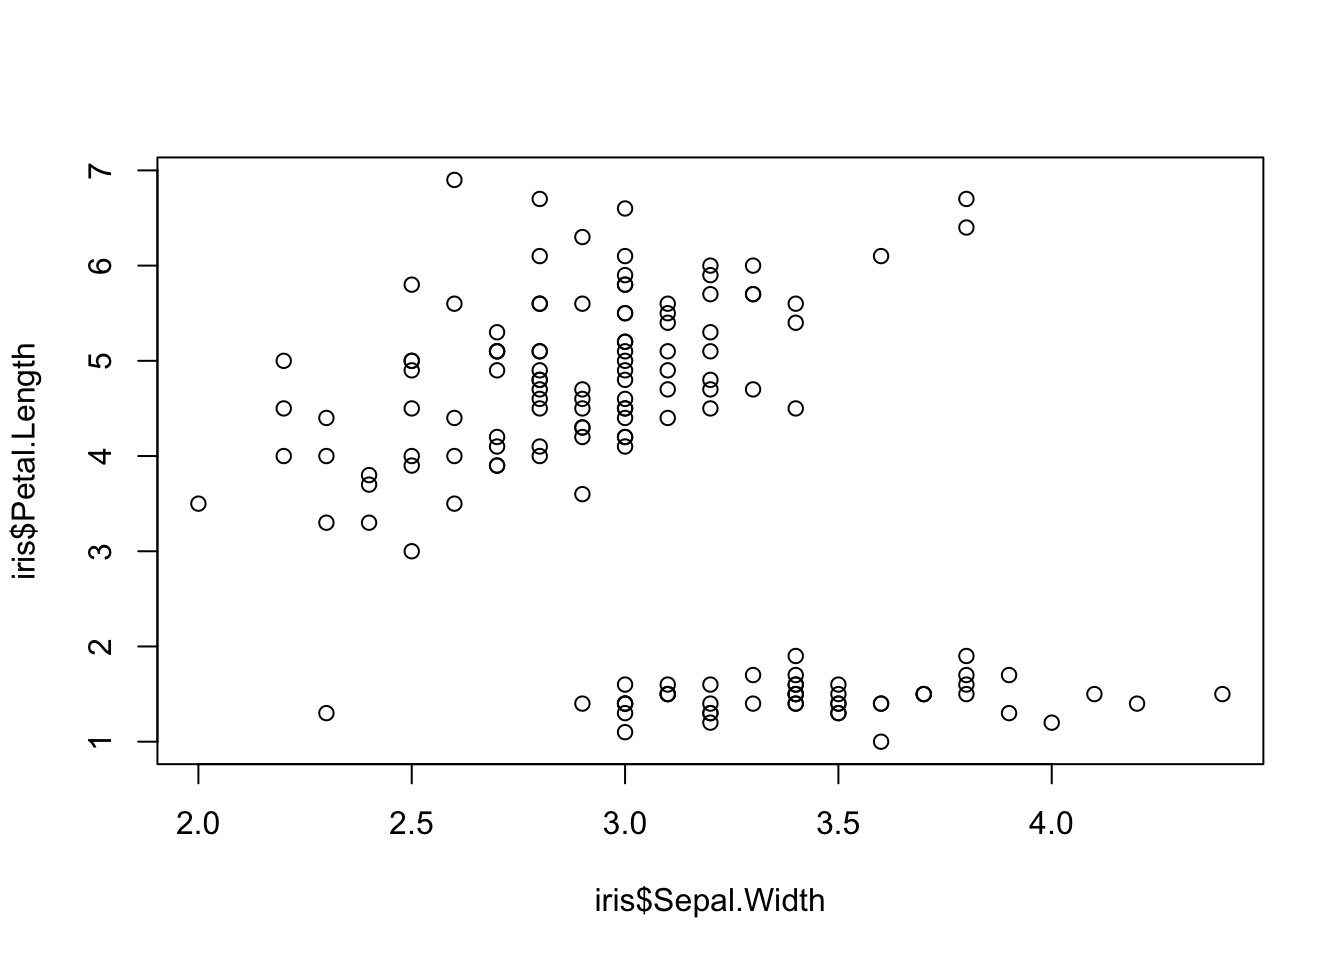
\includegraphics{texts_files/figure-latex/unnamed-chunk-50-1.pdf}

\begin{Shaded}
\begin{Highlighting}[]
\KeywordTok{plot}\NormalTok{(iris}\OperatorTok{$}\NormalTok{Sepal.Width, iris}\OperatorTok{$}\NormalTok{Petal.Length, }\DataTypeTok{col =}\NormalTok{ iris}\OperatorTok{$}\NormalTok{Species, }\DataTypeTok{pch =} \DecValTok{19}\NormalTok{)}
\KeywordTok{legend}\NormalTok{(}\StringTok{"topright"}\NormalTok{,}\DataTypeTok{legend=}\KeywordTok{levels}\NormalTok{(iris}\OperatorTok{$}\NormalTok{Species), }\DataTypeTok{col =} \DecValTok{1}\OperatorTok{:}\DecValTok{3}\NormalTok{, }\DataTypeTok{pch =} \DecValTok{19}\NormalTok{)}
\end{Highlighting}
\end{Shaded}

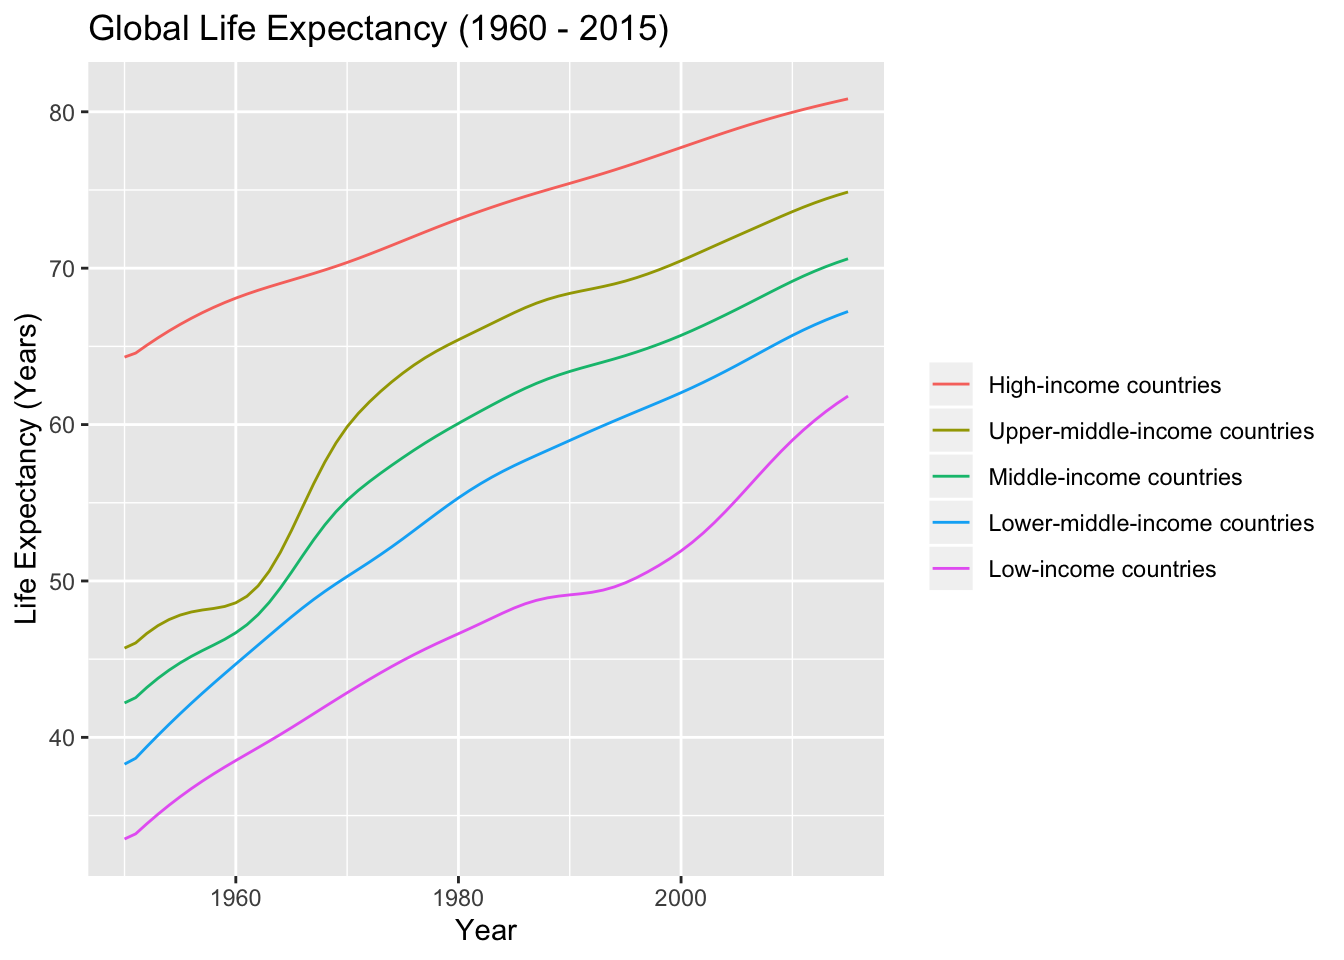
\includegraphics{texts_files/figure-latex/unnamed-chunk-51-1.pdf}

\hypertarget{hist}{%
\subsection*{\texorpdfstring{\textbf{hist}}{hist}}\label{hist}}
\addcontentsline{toc}{subsection}{\textbf{hist}}

\begin{Shaded}
\begin{Highlighting}[]
\KeywordTok{library}\NormalTok{(notitia)}
\NormalTok{police <-}\StringTok{ }\NormalTok{chi_emps[chi_emps}\OperatorTok{$}\NormalTok{Department }\OperatorTok{==}\StringTok{ "POLICE"}\NormalTok{, ]}
\KeywordTok{hist}\NormalTok{(police}\OperatorTok{$}\NormalTok{AnnualSalary)}
\end{Highlighting}
\end{Shaded}

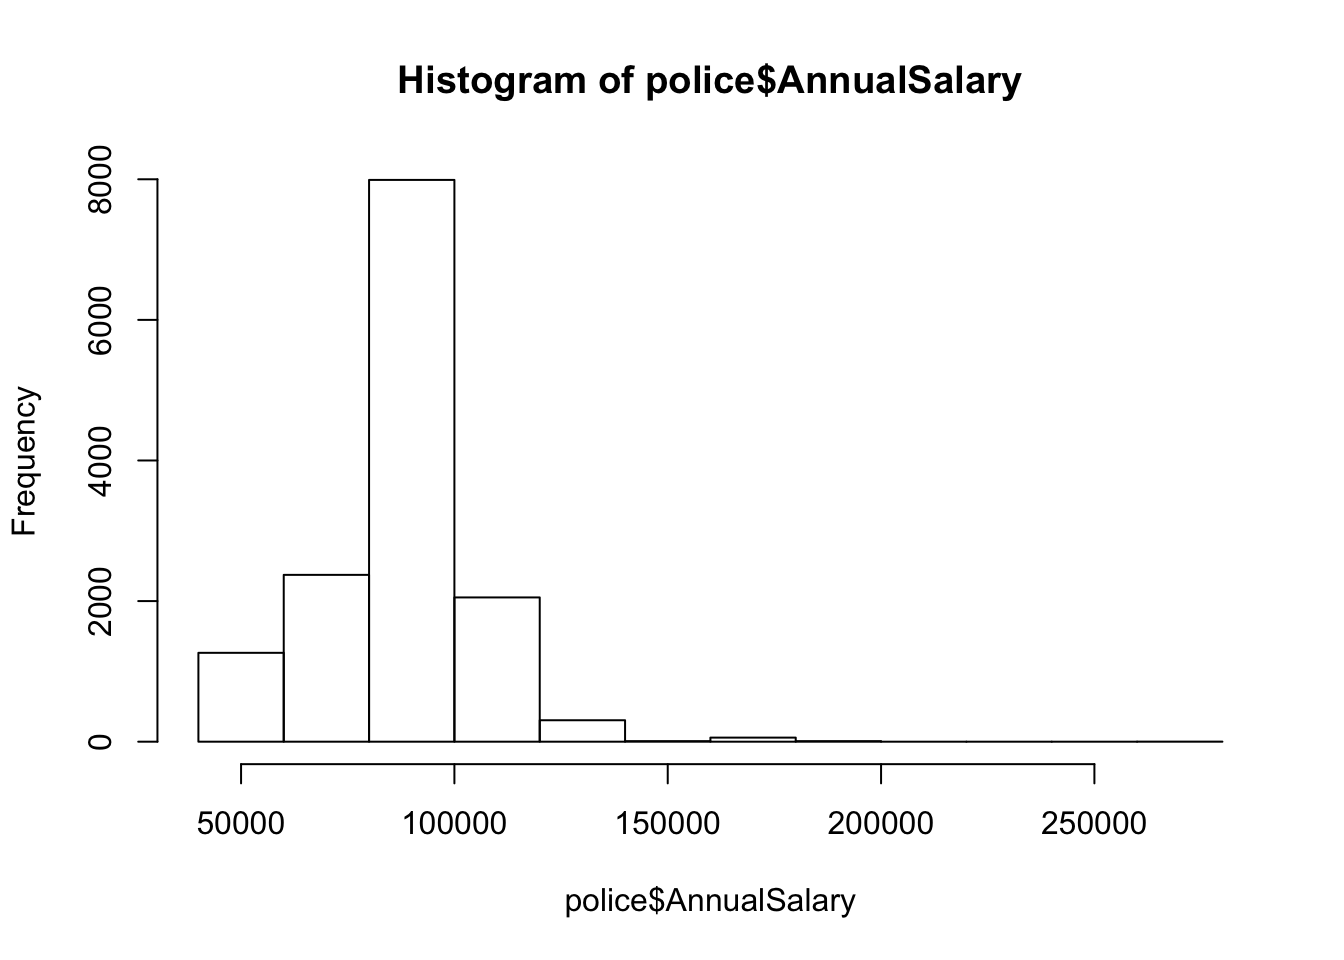
\includegraphics{texts_files/figure-latex/unnamed-chunk-52-1.pdf}

\hypertarget{barplot}{%
\subsection*{\texorpdfstring{\textbf{barplot}}{barplot}}\label{barplot}}
\addcontentsline{toc}{subsection}{\textbf{barplot}}

\hypertarget{boxplot}{%
\subsection*{\texorpdfstring{\textbf{boxplot}}{boxplot}}\label{boxplot}}
\addcontentsline{toc}{subsection}{\textbf{boxplot}}

\hypertarget{plotting-with-qplot}{%
\chapter{\texorpdfstring{Plotting with \textbf{qplot}}{Plotting with qplot}}\label{plotting-with-qplot}}

\begin{Shaded}
\begin{Highlighting}[]
\KeywordTok{library}\NormalTok{(ggplot2)}
\end{Highlighting}
\end{Shaded}

\hypertarget{plotquantities}{%
\section*{Quantities or Proportions}\label{plotquantities}}
\addcontentsline{toc}{section}{Quantities or Proportions}

\begin{Shaded}
\begin{Highlighting}[]
\KeywordTok{library}\NormalTok{(dplyr)}
\NormalTok{apple_}\DecValTok{2018}\NormalTok{ <-}\StringTok{ }\KeywordTok{filter}\NormalTok{(apple, Year }\OperatorTok{==}\StringTok{ }\DecValTok{2018}\NormalTok{) }\OperatorTok\StringTok{ }
\StringTok{  }\KeywordTok{group_by}\NormalTok{(Product) }\OperatorTok\StringTok{ }\KeywordTok{summarise}\NormalTok{(}\DataTypeTok{Revenue =} \KeywordTok{sum}\NormalTok{(Revenue))}
\NormalTok{apple_}\DecValTok{2018}
\end{Highlighting}
\end{Shaded}

\begin{verbatim}
## # A tibble: 5 x 2
##   Product        Revenue
##   <chr>            <dbl>
## 1 iPad             18805
## 2 iPhone          166699
## 3 Mac              25484
## 4 Other Products   17417
## 5 Services         37190
\end{verbatim}

\hypertarget{qplotbars}{%
\subsection*{Bar Charts}\label{qplotbars}}
\addcontentsline{toc}{subsection}{Bar Charts}

\begin{Shaded}
\begin{Highlighting}[]
\KeywordTok{qplot}\NormalTok{(}\DataTypeTok{x =}\NormalTok{ Product, }\DataTypeTok{data =}\NormalTok{ apple_}\DecValTok{2018}\NormalTok{, }\DataTypeTok{geom =} \StringTok{"bar"}\NormalTok{, }\DataTypeTok{weight =}\NormalTok{ Revenue) }
\end{Highlighting}
\end{Shaded}

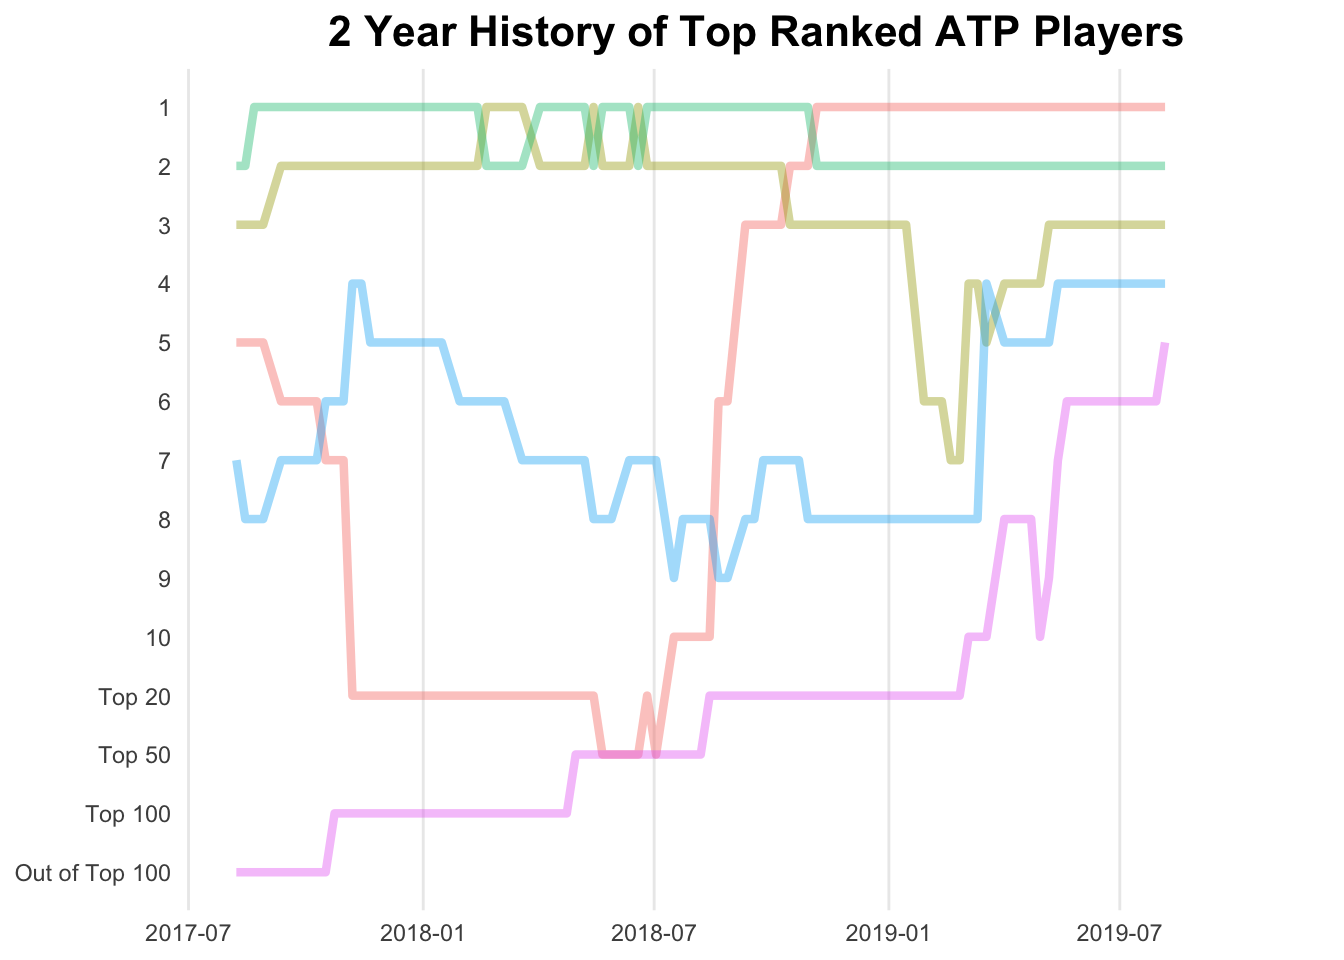
\includegraphics{texts_files/figure-latex/unnamed-chunk-56-1.pdf}

\begin{Shaded}
\begin{Highlighting}[]
\KeywordTok{qplot}\NormalTok{(}\DataTypeTok{x =}\NormalTok{ Product, }\DataTypeTok{data =}\NormalTok{ apple_}\DecValTok{2018}\NormalTok{, }\DataTypeTok{geom =} \StringTok{"bar"}\NormalTok{, }\DataTypeTok{weight =}\NormalTok{ Revenue, }\DataTypeTok{fill =} \KeywordTok{I}\NormalTok{(}\StringTok{"royalblue"}\NormalTok{)) }
\end{Highlighting}
\end{Shaded}

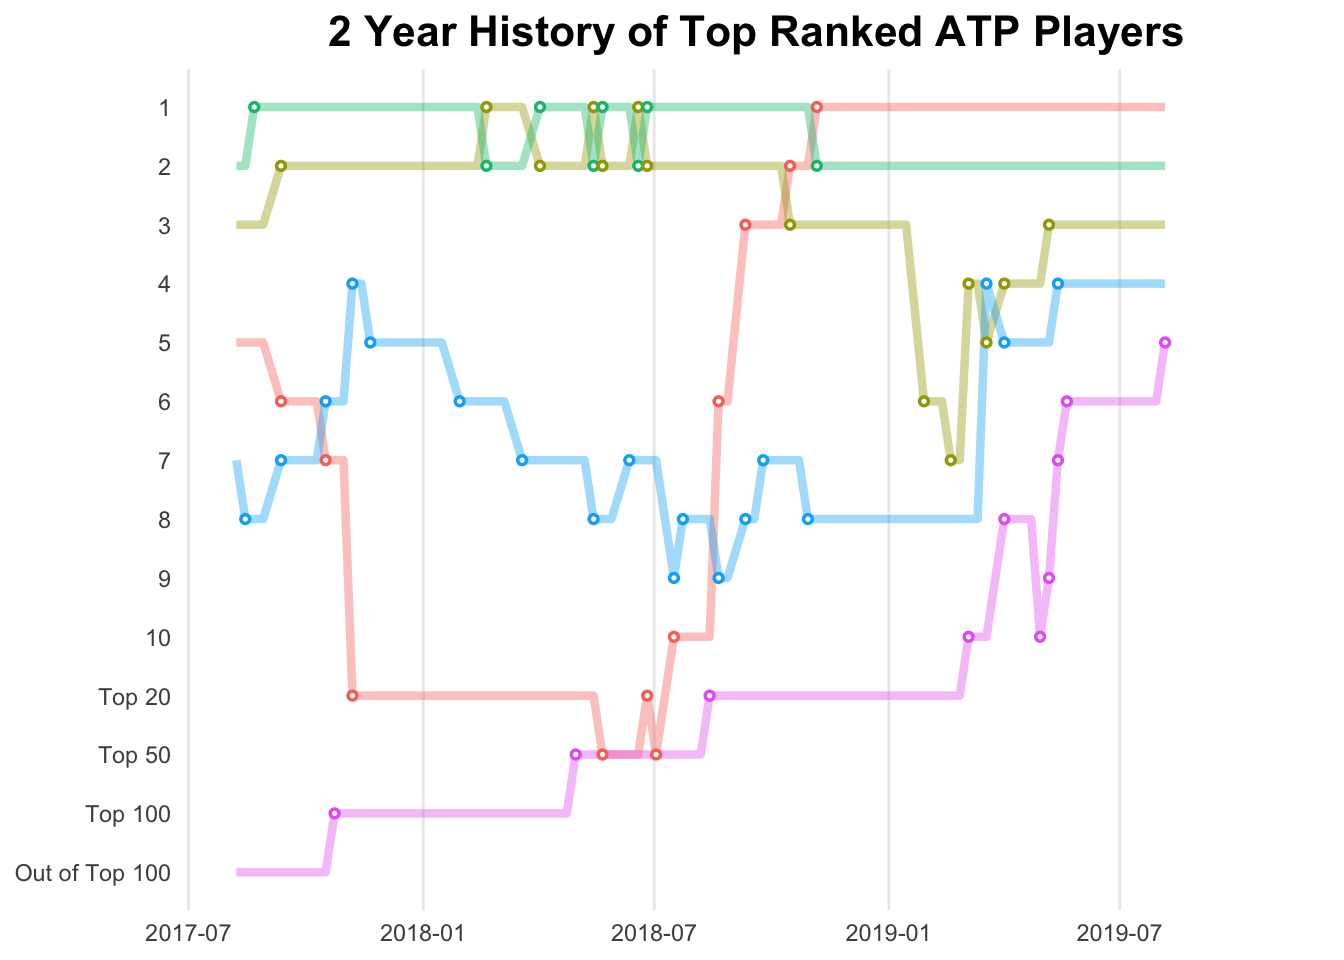
\includegraphics{texts_files/figure-latex/unnamed-chunk-57-1.pdf}

\begin{Shaded}
\begin{Highlighting}[]
\KeywordTok{qplot}\NormalTok{(}\DataTypeTok{x =}\NormalTok{ Year, }\DataTypeTok{data =}\NormalTok{ apple, }\DataTypeTok{geom =} \StringTok{"bar"}\NormalTok{, }\DataTypeTok{weight =}\NormalTok{ Revenue, }\DataTypeTok{fill =}\NormalTok{ Product)}
\end{Highlighting}
\end{Shaded}

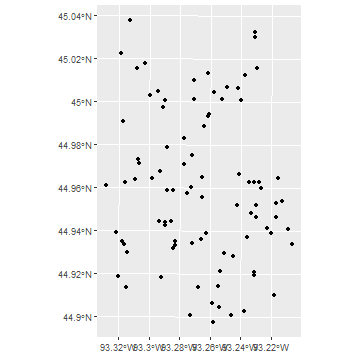
\includegraphics{texts_files/figure-latex/unnamed-chunk-58-1.pdf}

\begin{Shaded}
\begin{Highlighting}[]
\KeywordTok{qplot}\NormalTok{(}\DataTypeTok{x =}\NormalTok{ Year, }\DataTypeTok{data =}\NormalTok{ apple, }\DataTypeTok{geom =} \StringTok{"bar"}\NormalTok{, }\DataTypeTok{weight =}\NormalTok{ Revenue, }\DataTypeTok{fill =}\NormalTok{ Product)}
\end{Highlighting}
\end{Shaded}

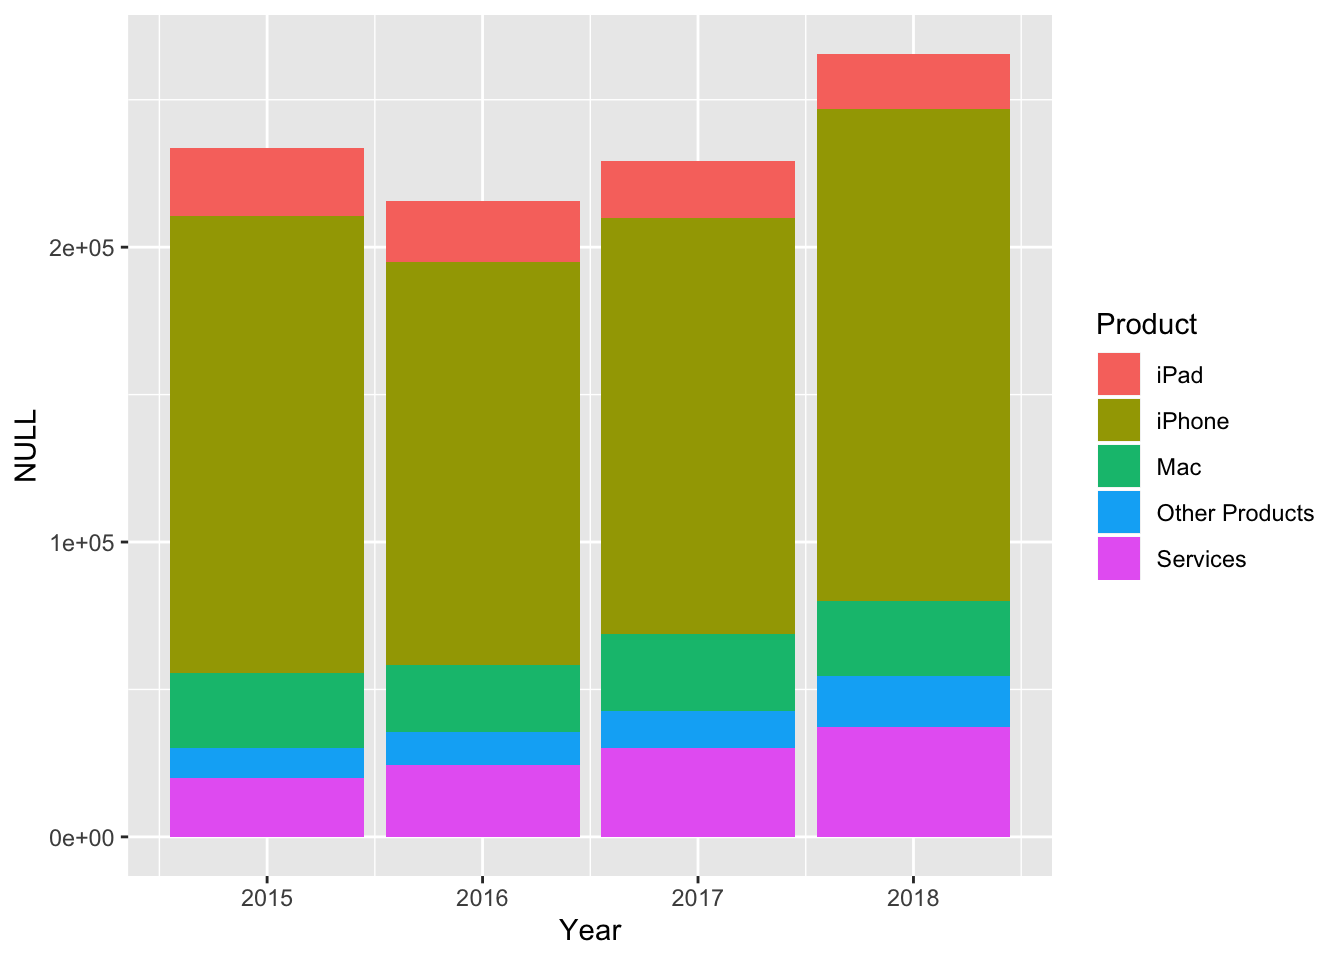
\includegraphics{texts_files/figure-latex/unnamed-chunk-59-1.pdf}

\hypertarget{plotdistributions}{%
\section*{Distributions}\label{plotdistributions}}
\addcontentsline{toc}{section}{Distributions}

Geometries:
- \emph{histogram}
- \emph{boxplot}
- \emph{density}

\begin{Shaded}
\begin{Highlighting}[]
\KeywordTok{library}\NormalTok{(notitia)}
\NormalTok{large_depts <-}\StringTok{ }\NormalTok{chi_emps[chi_emps}\OperatorTok{$}\NormalTok{Department }\OperatorTok\StringTok{ }\KeywordTok{c}\NormalTok{(}\StringTok{"POLICE"}\NormalTok{, }\StringTok{"FIRE"}\NormalTok{, }\StringTok{"STREETS & SAN"}\NormalTok{), ]}
\KeywordTok{table}\NormalTok{(large_depts}\OperatorTok{$}\NormalTok{Department)}
\end{Highlighting}
\end{Shaded}

\begin{verbatim}
## 
##          FIRE        POLICE STREETS & SAN 
##          4633         14083          2206
\end{verbatim}

\hypertarget{qplothist}{%
\subsection*{Histograms}\label{qplothist}}
\addcontentsline{toc}{subsection}{Histograms}

\begin{Shaded}
\begin{Highlighting}[]
\KeywordTok{qplot}\NormalTok{(}\DataTypeTok{x =}\NormalTok{ AnnualSalary, }\DataTypeTok{data =}\NormalTok{ large_depts, }\DataTypeTok{geom =} \StringTok{"histogram"}\NormalTok{) }
\end{Highlighting}
\end{Shaded}

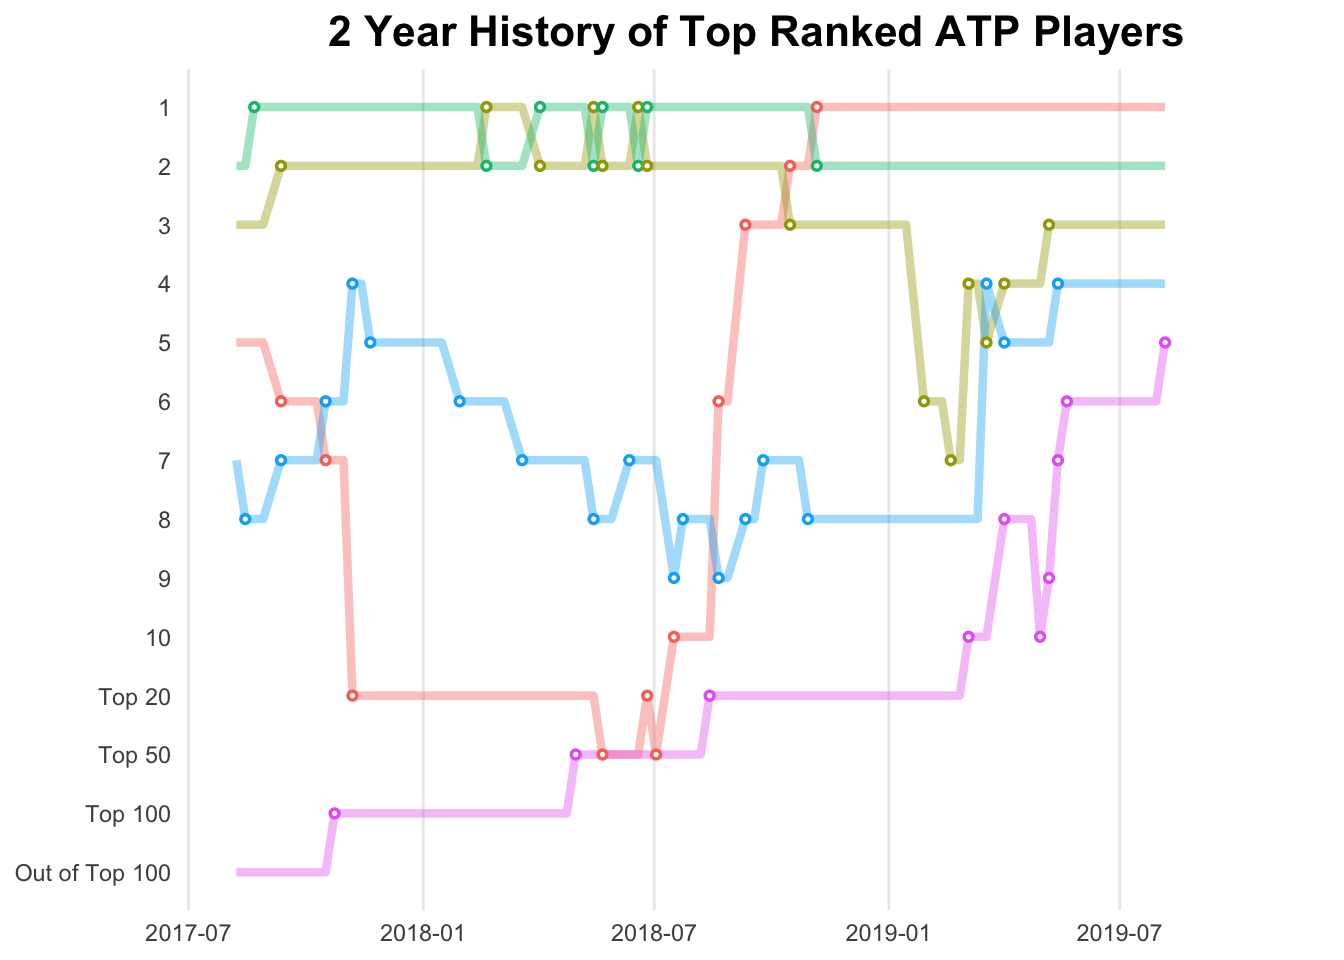
\includegraphics{texts_files/figure-latex/unnamed-chunk-61-1.pdf}

\begin{Shaded}
\begin{Highlighting}[]
\KeywordTok{qplot}\NormalTok{(}\DataTypeTok{x =}\NormalTok{ AnnualSalary, }\DataTypeTok{data =}\NormalTok{ large_depts, }\DataTypeTok{geom =} \StringTok{"histogram"}\NormalTok{, }\DataTypeTok{fill =} \KeywordTok{I}\NormalTok{(}\StringTok{"orange"}\NormalTok{), }\DataTypeTok{colour =} \KeywordTok{I}\NormalTok{(}\StringTok{"black"}\NormalTok{)) }
\end{Highlighting}
\end{Shaded}

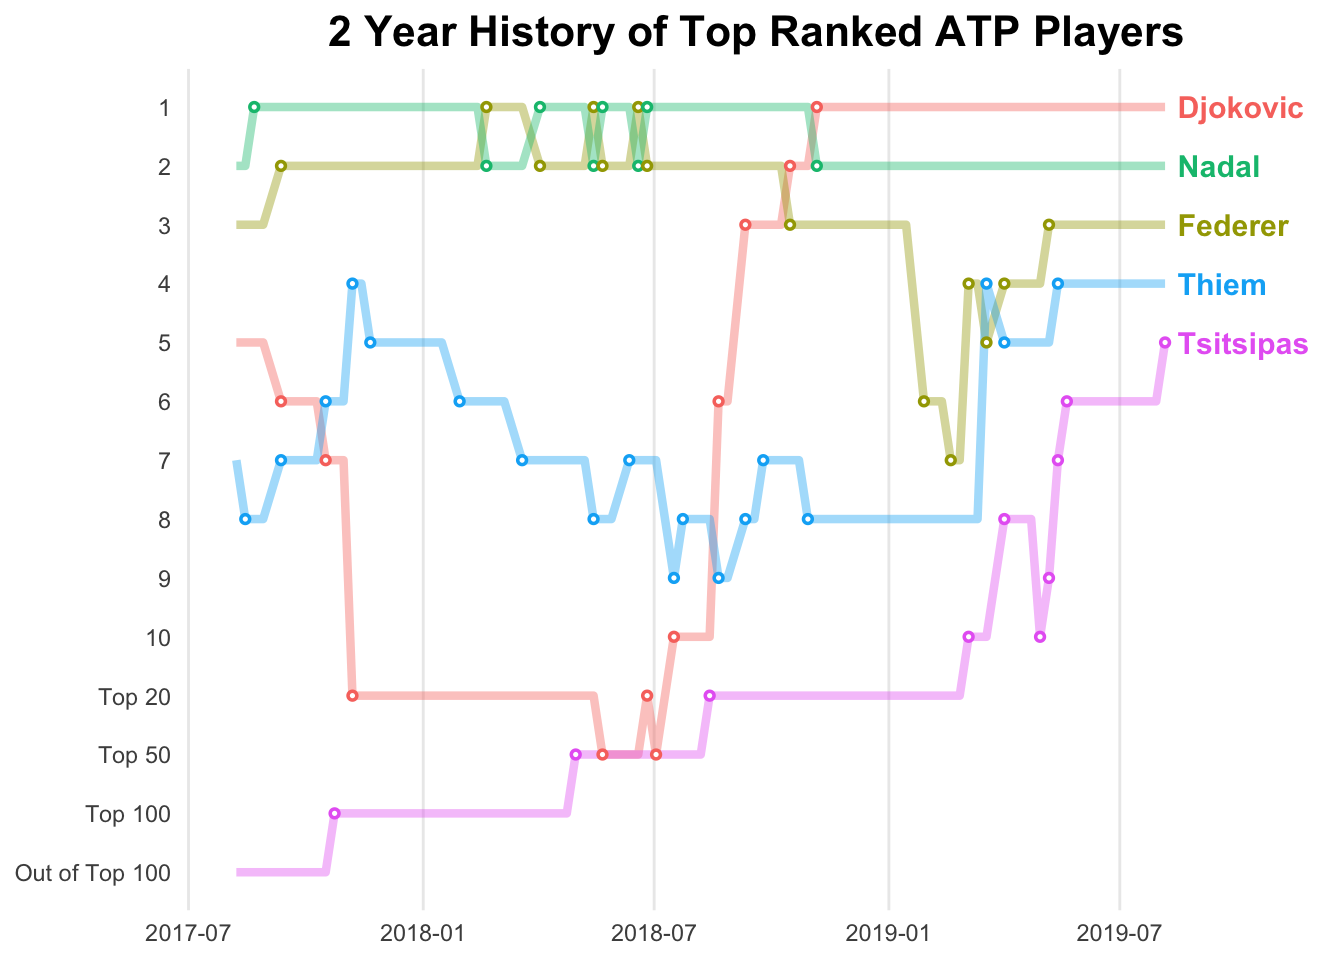
\includegraphics{texts_files/figure-latex/unnamed-chunk-62-1.pdf}

\begin{Shaded}
\begin{Highlighting}[]
\KeywordTok{library}\NormalTok{(ggplot2)}
\KeywordTok{qplot}\NormalTok{(}\DataTypeTok{x =}\NormalTok{ AnnualSalary, }\DataTypeTok{data =}\NormalTok{ large_depts, }\DataTypeTok{geom =} \StringTok{"histogram"}\NormalTok{, }\DataTypeTok{facets =}\NormalTok{ Department}\OperatorTok{~}\NormalTok{.)}
\end{Highlighting}
\end{Shaded}

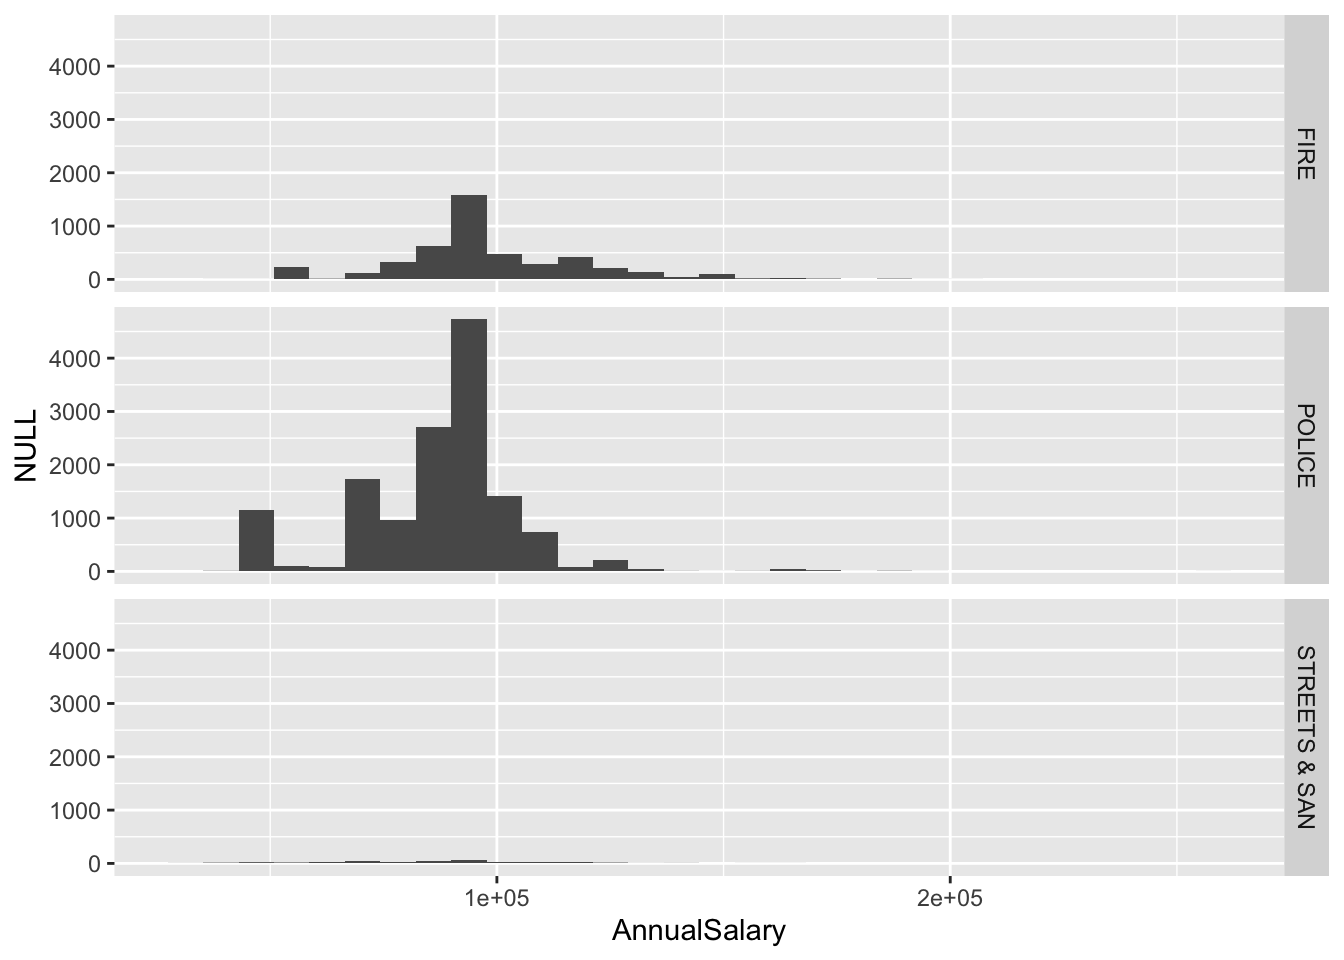
\includegraphics{texts_files/figure-latex/unnamed-chunk-63-1.pdf}

\begin{Shaded}
\begin{Highlighting}[]
\KeywordTok{qplot}\NormalTok{(}\DataTypeTok{x =}\NormalTok{ AnnualSalary, }\DataTypeTok{data =}\NormalTok{ large_depts, }\DataTypeTok{geom =} \StringTok{"histogram"}\NormalTok{, }\DataTypeTok{facets =}\NormalTok{ Department}\OperatorTok{~}\NormalTok{., }\DataTypeTok{scale =} \StringTok{"free_y"}\NormalTok{) }
\end{Highlighting}
\end{Shaded}

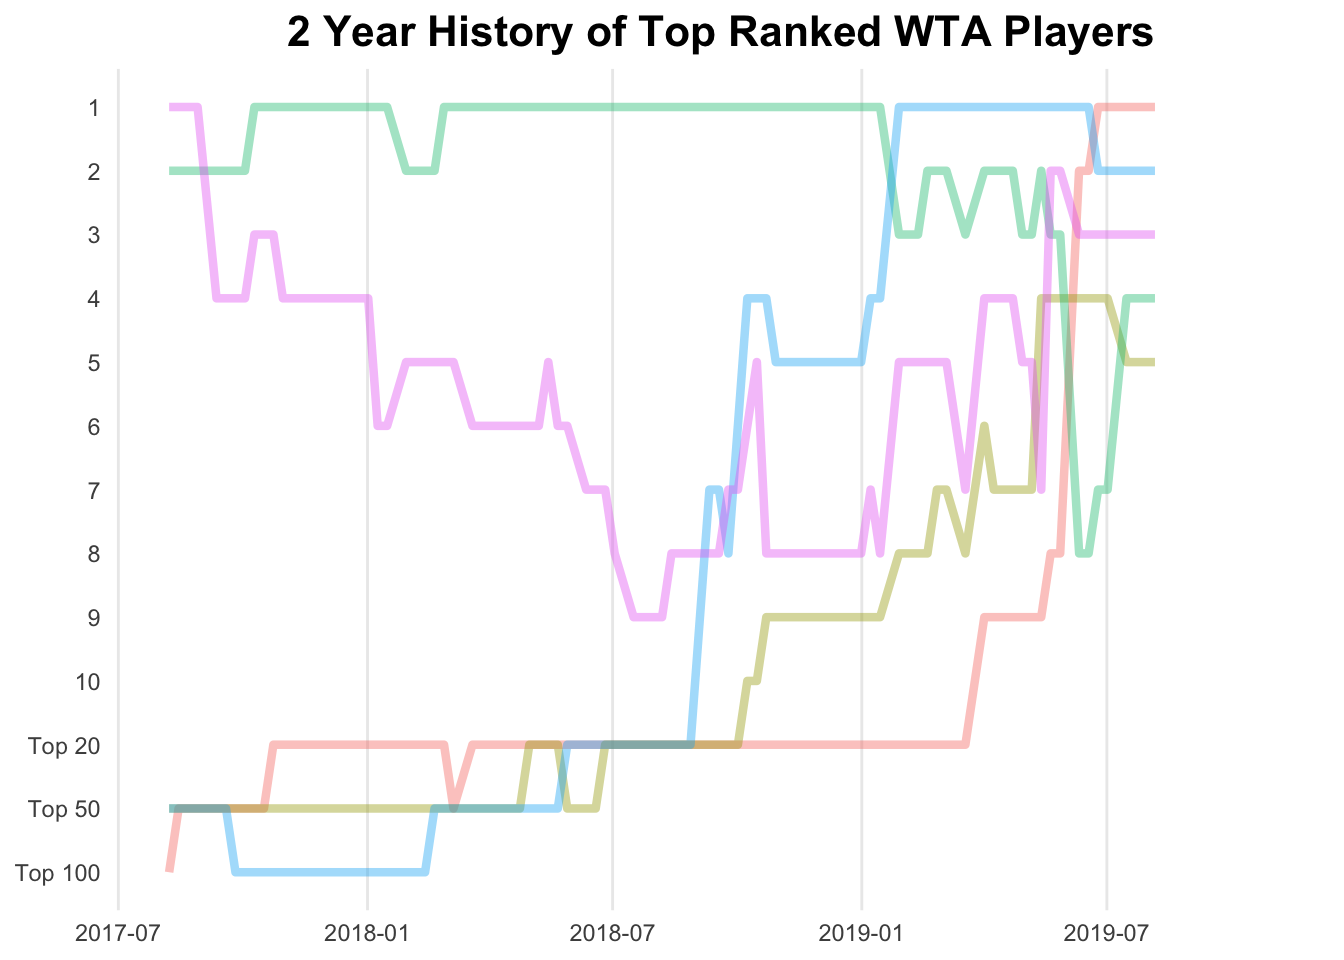
\includegraphics{texts_files/figure-latex/unnamed-chunk-64-1.pdf}

\begin{Shaded}
\begin{Highlighting}[]
\KeywordTok{qplot}\NormalTok{(}\DataTypeTok{x =}\NormalTok{ AnnualSalary, }\DataTypeTok{data =}\NormalTok{ large_depts, }\DataTypeTok{geom =} \StringTok{"histogram"}\NormalTok{, }\DataTypeTok{fill =}\NormalTok{ Department) }\OperatorTok{+}\StringTok{ }
\StringTok{  }\KeywordTok{facet_wrap}\NormalTok{(Department}\OperatorTok{~}\NormalTok{., }\DataTypeTok{scales =} \StringTok{"free_y"}\NormalTok{, }\DataTypeTok{ncol =} \DecValTok{1}\NormalTok{)  }
\end{Highlighting}
\end{Shaded}

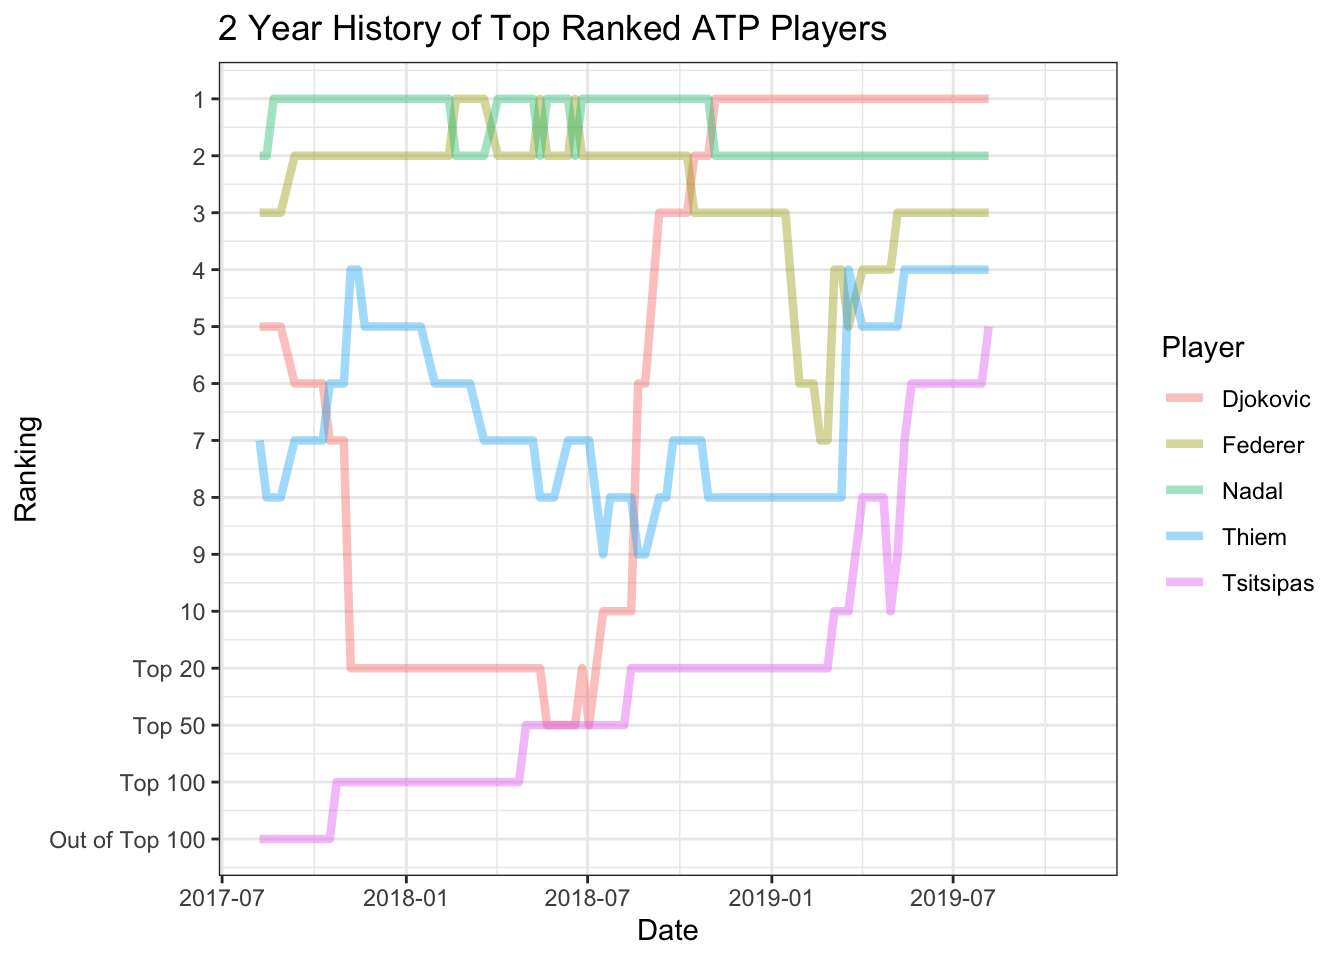
\includegraphics{texts_files/figure-latex/unnamed-chunk-65-1.pdf}

\begin{Shaded}
\begin{Highlighting}[]
\KeywordTok{qplot}\NormalTok{(}\DataTypeTok{x =}\NormalTok{ AnnualSalary, }\DataTypeTok{data =}\NormalTok{ large_depts, }\DataTypeTok{geom =} \StringTok{"histogram"}\NormalTok{, }\DataTypeTok{fill =}\NormalTok{ Department, }\DataTypeTok{colour =} \KeywordTok{I}\NormalTok{(}\StringTok{"black"}\NormalTok{)) }\OperatorTok{+}\StringTok{ }
\StringTok{  }\KeywordTok{facet_wrap}\NormalTok{(Department}\OperatorTok{~}\NormalTok{., }\DataTypeTok{scales =} \StringTok{"free_y"}\NormalTok{, }\DataTypeTok{ncol =} \DecValTok{1}\NormalTok{)  }
\end{Highlighting}
\end{Shaded}

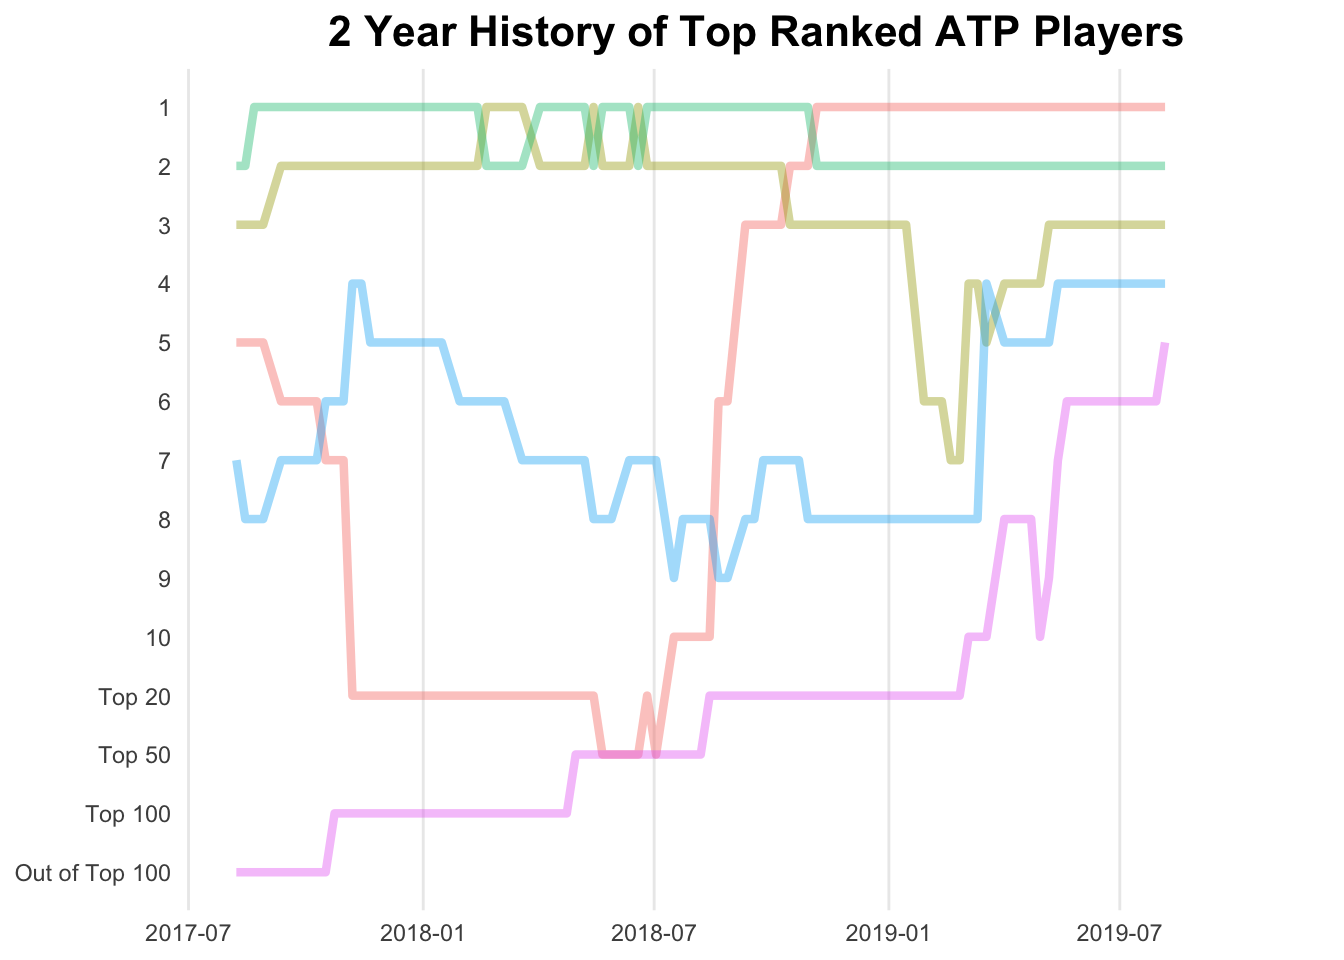
\includegraphics{texts_files/figure-latex/unnamed-chunk-66-1.pdf}

\hypertarget{qplotdensity}{%
\subsection*{Density plots}\label{qplotdensity}}
\addcontentsline{toc}{subsection}{Density plots}

\begin{Shaded}
\begin{Highlighting}[]
\KeywordTok{qplot}\NormalTok{(}\DataTypeTok{x =}\NormalTok{ AnnualSalary, }\DataTypeTok{data =}\NormalTok{ large_depts, }\DataTypeTok{geom =} \StringTok{"density"}\NormalTok{, }\DataTypeTok{fill =}\NormalTok{ Department, }\DataTypeTok{alpha =} \KeywordTok{I}\NormalTok{(}\FloatTok{0.3}\NormalTok{)) }
\end{Highlighting}
\end{Shaded}

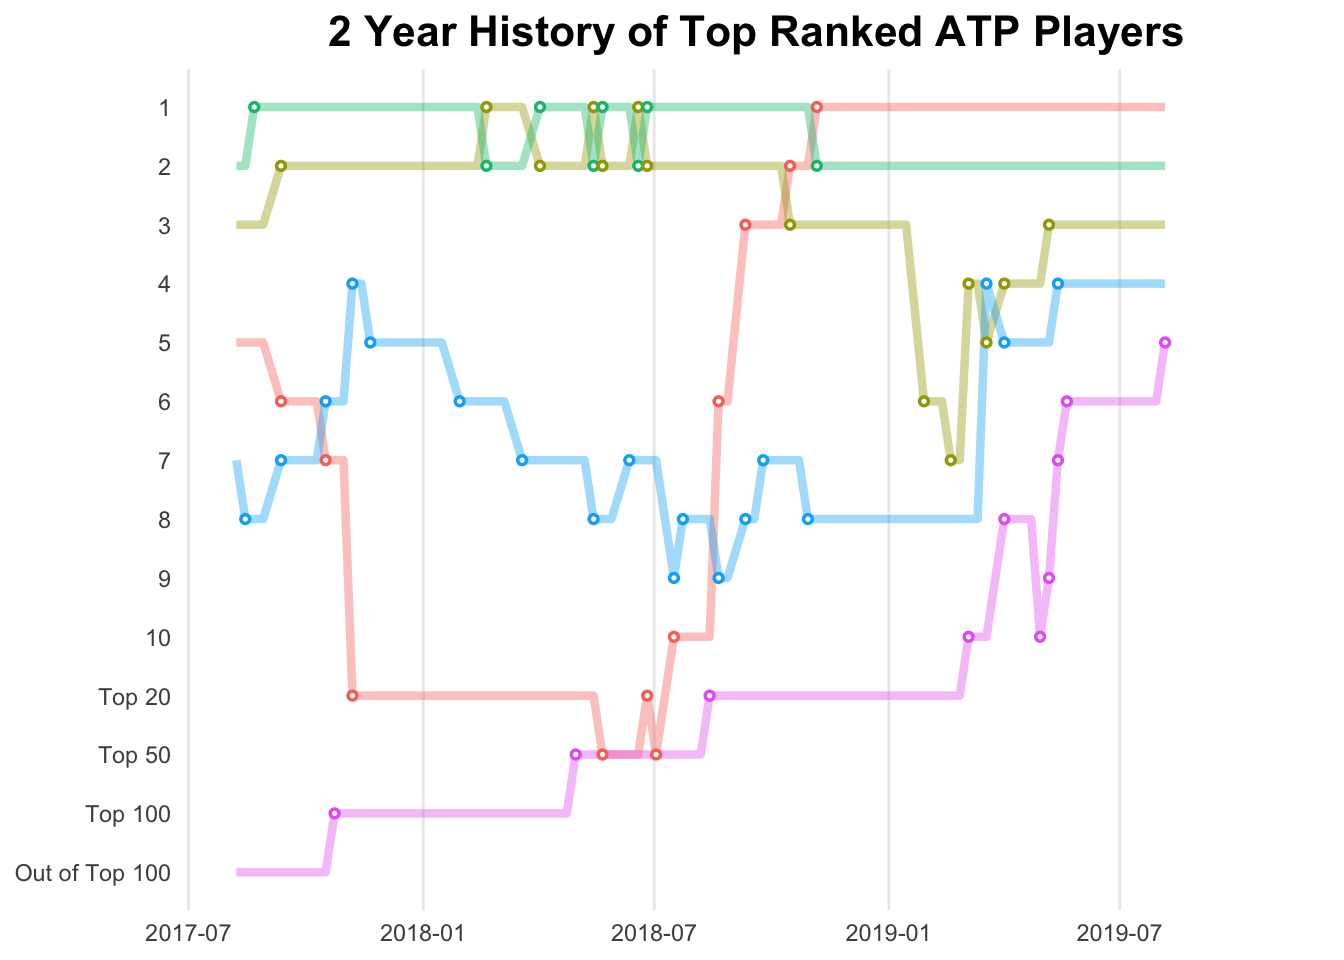
\includegraphics{texts_files/figure-latex/unnamed-chunk-67-1.pdf}

\begin{Shaded}
\begin{Highlighting}[]
\KeywordTok{qplot}\NormalTok{(}\DataTypeTok{x =}\NormalTok{ AnnualSalary, }\DataTypeTok{data =}\NormalTok{ large_depts, }\DataTypeTok{geom =} \StringTok{"density"}\NormalTok{, }\DataTypeTok{fill =}\NormalTok{ Department, }\DataTypeTok{alpha =} \KeywordTok{I}\NormalTok{(}\FloatTok{0.3}\NormalTok{)) }\OperatorTok{+}\StringTok{ }
\StringTok{  }\KeywordTok{facet_wrap}\NormalTok{(Department}\OperatorTok{~}\NormalTok{., }\DataTypeTok{ncol =} \DecValTok{1}\NormalTok{)}
\end{Highlighting}
\end{Shaded}

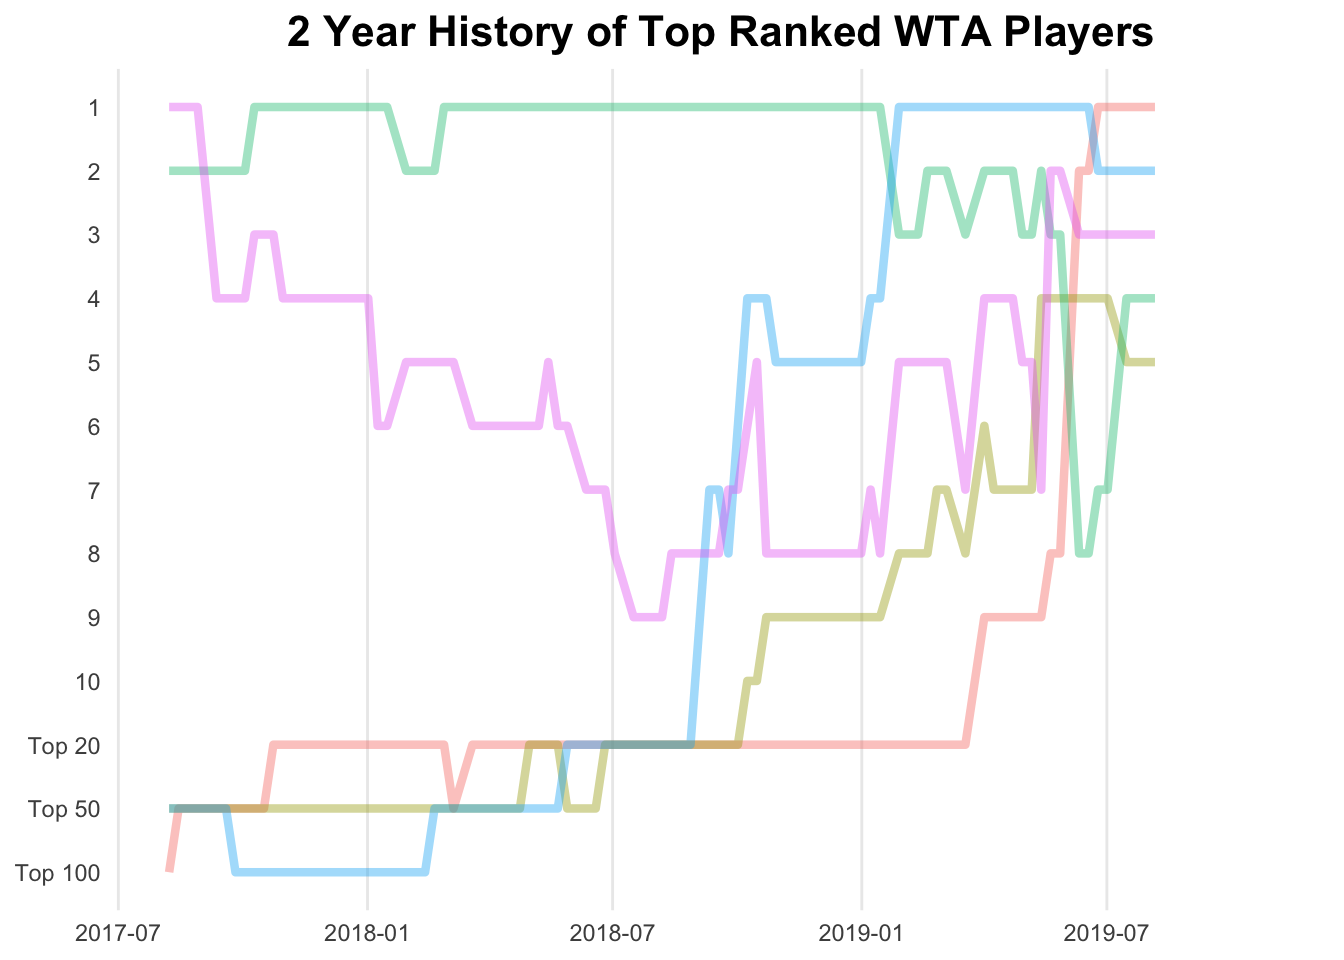
\includegraphics{texts_files/figure-latex/unnamed-chunk-68-1.pdf}

\hypertarget{qplotbox}{%
\subsection*{Box plots}\label{qplotbox}}
\addcontentsline{toc}{subsection}{Box plots}

\begin{Shaded}
\begin{Highlighting}[]
\KeywordTok{qplot}\NormalTok{(}\DataTypeTok{x =}\NormalTok{ Department, }\DataTypeTok{y =}\NormalTok{ AnnualSalary, }\DataTypeTok{data =}\NormalTok{ large_depts, }\DataTypeTok{geom =} \StringTok{"boxplot"}\NormalTok{) }
\end{Highlighting}
\end{Shaded}

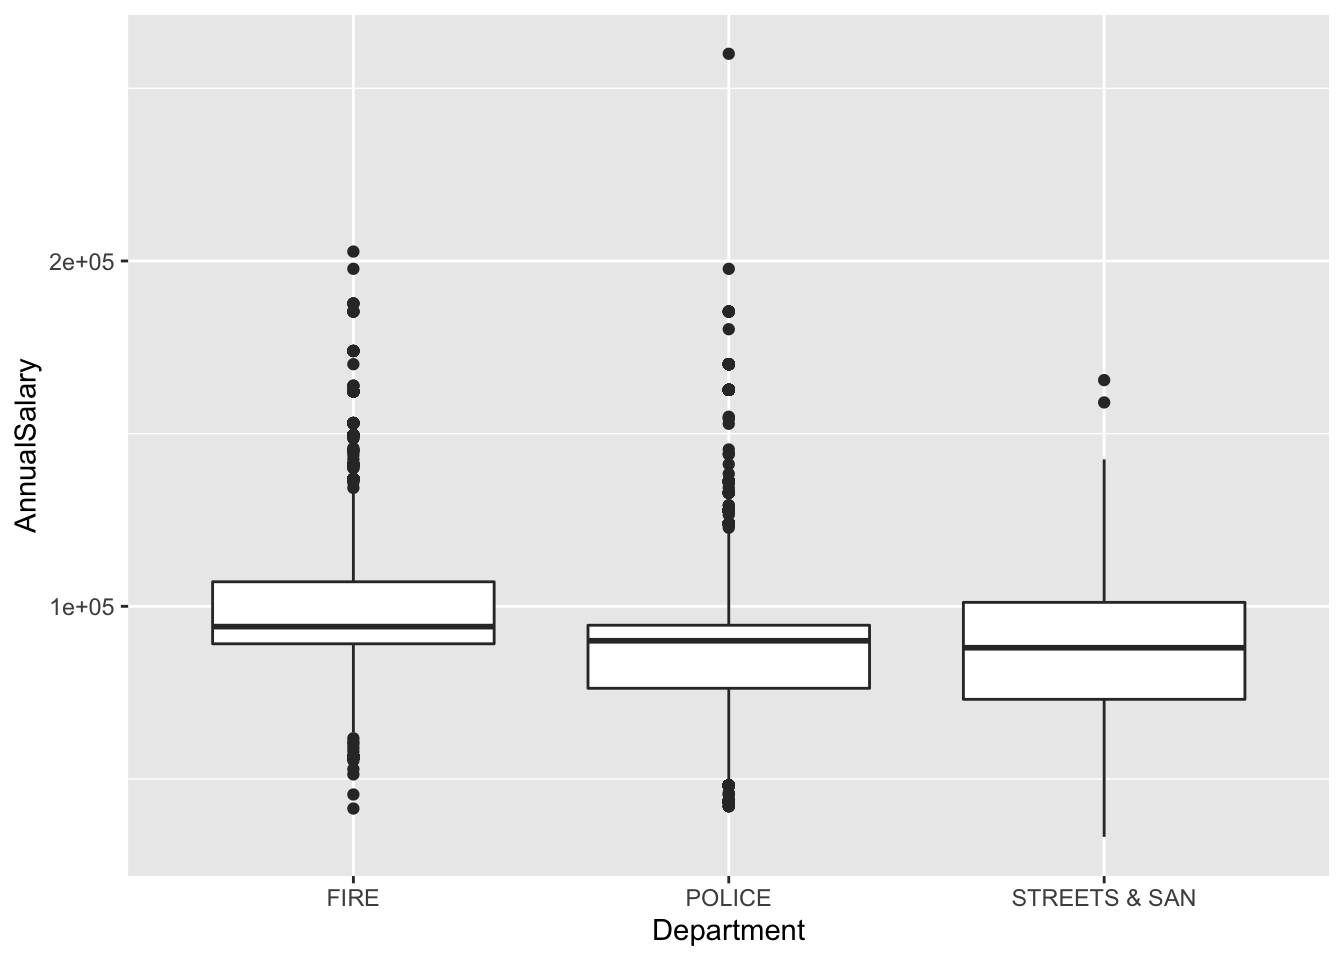
\includegraphics{texts_files/figure-latex/unnamed-chunk-69-1.pdf}

\hypertarget{plotxy}{%
\section*{x-y relationships}\label{plotxy}}
\addcontentsline{toc}{section}{x-y relationships}

\begin{Shaded}
\begin{Highlighting}[]
\KeywordTok{qplot}\NormalTok{(}\DataTypeTok{x =}\NormalTok{ Sepal.Width, }\DataTypeTok{y =}\NormalTok{ Sepal.Length, }\DataTypeTok{data =}\NormalTok{ iris, }\DataTypeTok{geom =} \StringTok{"point"}\NormalTok{)}
\end{Highlighting}
\end{Shaded}

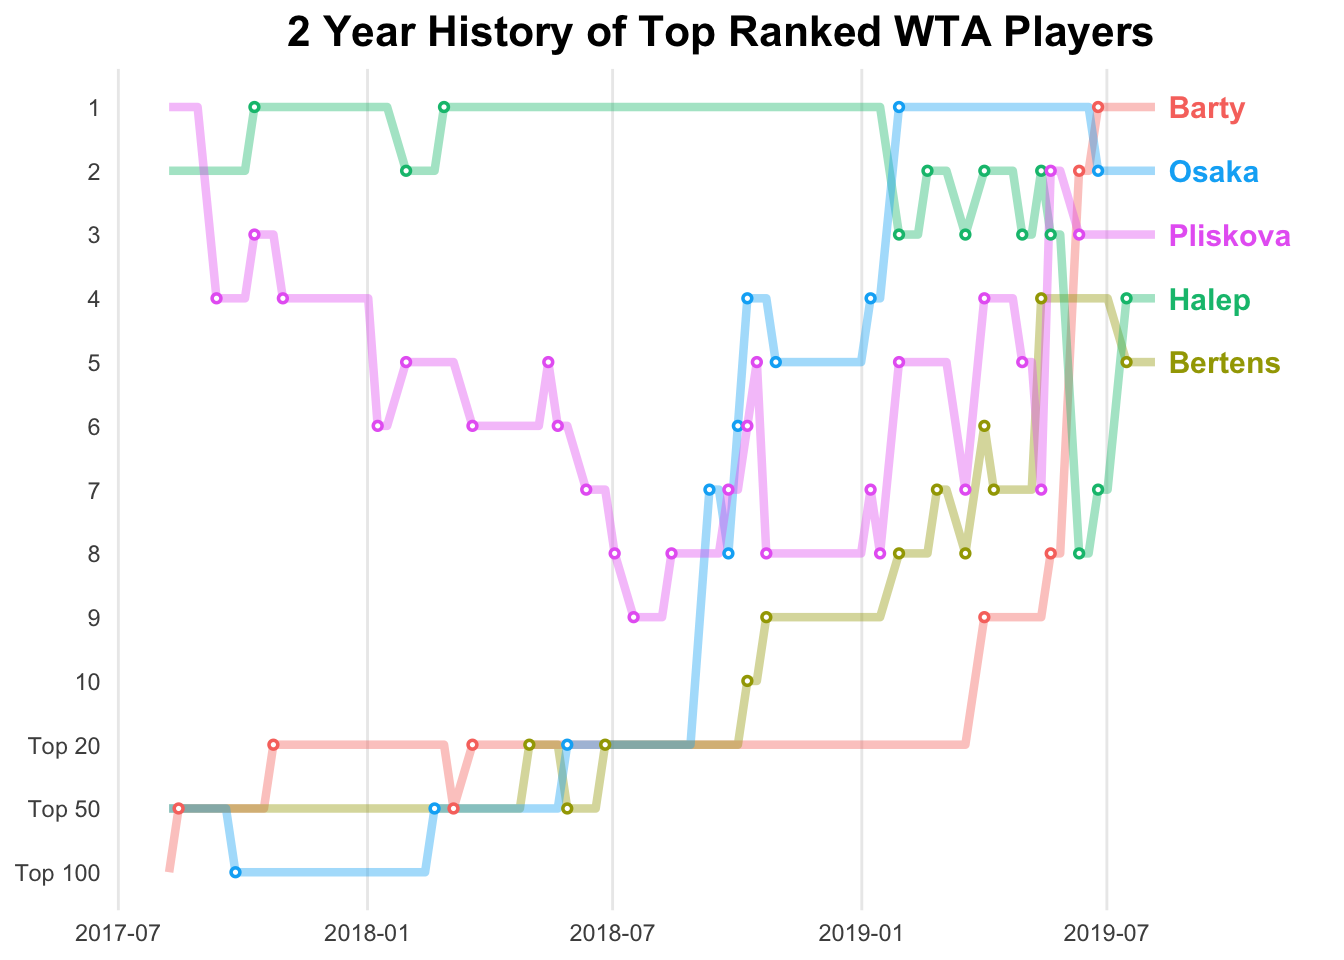
\includegraphics{texts_files/figure-latex/unnamed-chunk-70-1.pdf}

\begin{Shaded}
\begin{Highlighting}[]
\KeywordTok{qplot}\NormalTok{(}\DataTypeTok{x =}\NormalTok{ Sepal.Width, }\DataTypeTok{y =}\NormalTok{ Sepal.Length, }\DataTypeTok{data =}\NormalTok{ iris, }\DataTypeTok{colour =}\NormalTok{ Species, }\DataTypeTok{geom =} \StringTok{"point"}\NormalTok{)}
\end{Highlighting}
\end{Shaded}

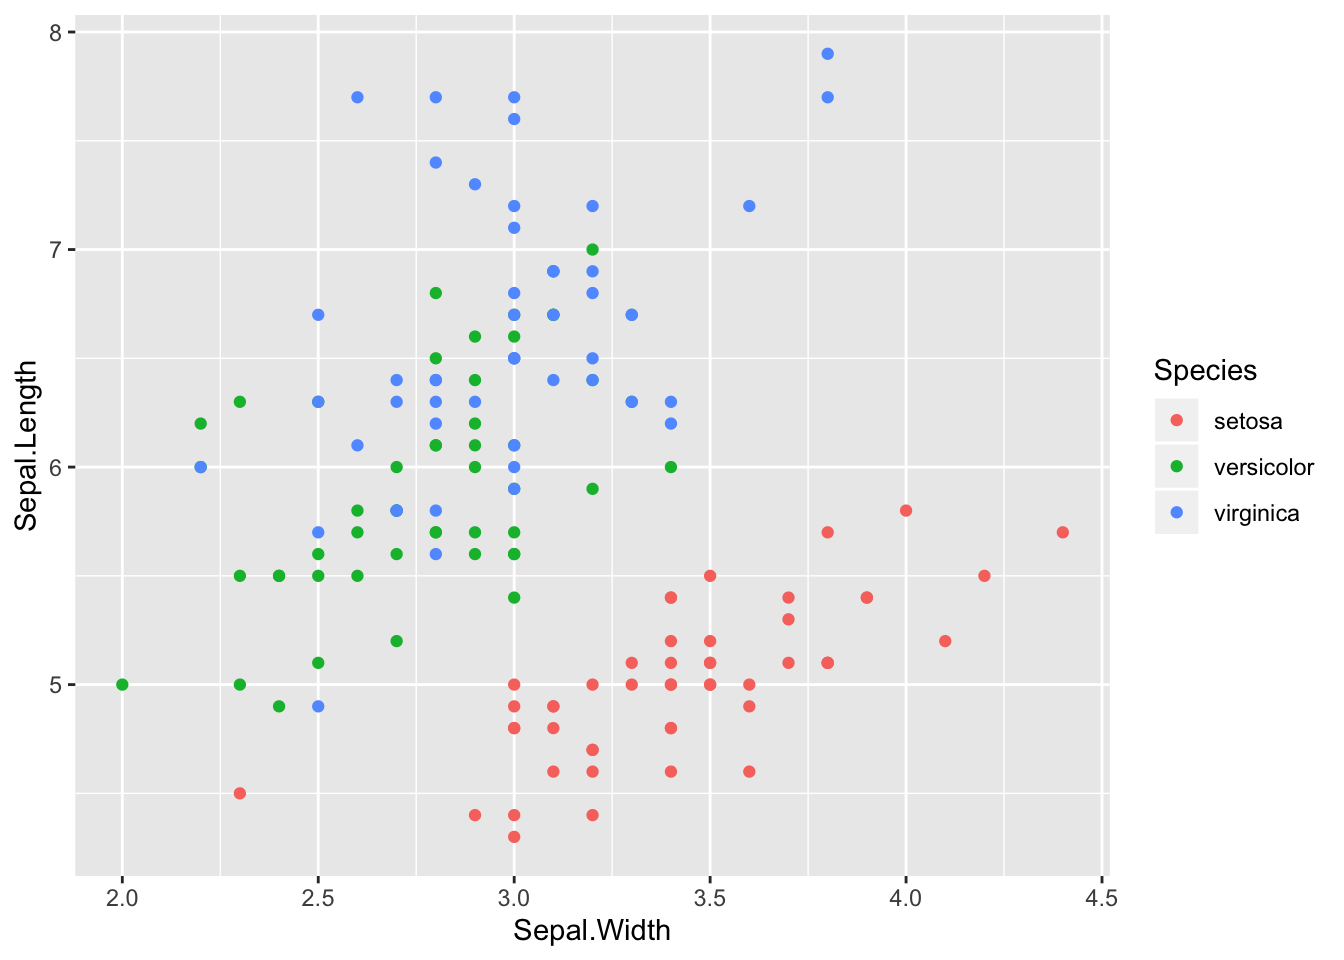
\includegraphics{texts_files/figure-latex/unnamed-chunk-71-1.pdf}

\hypertarget{plotts}{%
\subsection*{Time Series}\label{plotts}}
\addcontentsline{toc}{subsection}{Time Series}

\begin{Shaded}
\begin{Highlighting}[]
\NormalTok{apple}\OperatorTok{$}\NormalTok{X =}\StringTok{ }\KeywordTok{paste}\NormalTok{(apple}\OperatorTok{$}\NormalTok{Year, apple}\OperatorTok{$}\NormalTok{Quarter)}
\KeywordTok{qplot}\NormalTok{(}\DataTypeTok{x =}\NormalTok{ X, }\DataTypeTok{y =}\NormalTok{ Revenue, }\DataTypeTok{data =}\NormalTok{ apple, }\DataTypeTok{group =}\NormalTok{ Product, }\DataTypeTok{geom =} \KeywordTok{c}\NormalTok{(}\StringTok{"point"}\NormalTok{, }\StringTok{"line"}\NormalTok{))}
\end{Highlighting}
\end{Shaded}

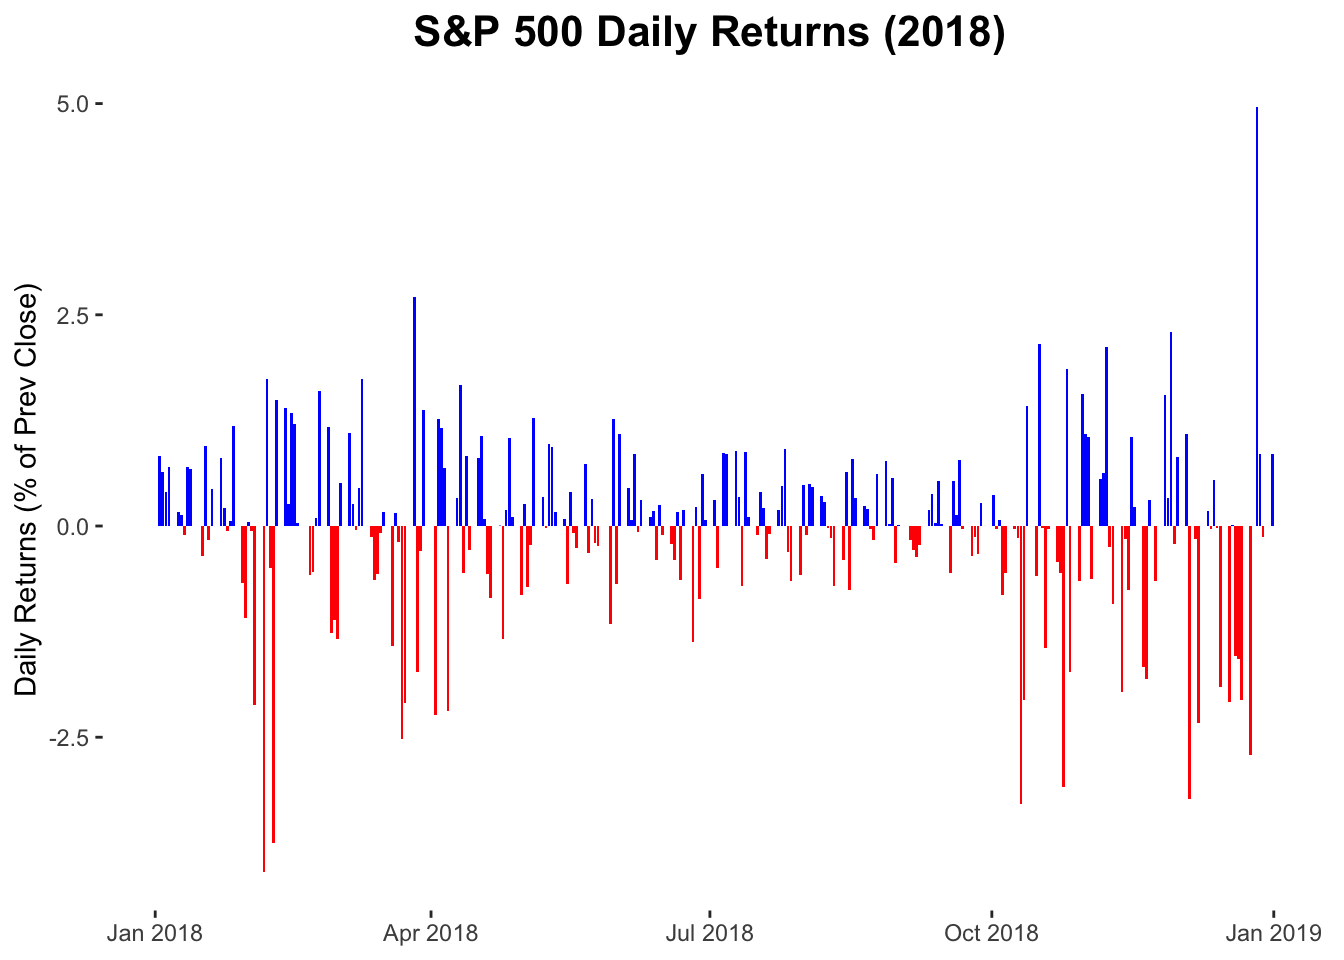
\includegraphics{texts_files/figure-latex/unnamed-chunk-72-1.pdf}

\begin{Shaded}
\begin{Highlighting}[]
\NormalTok{apple}\OperatorTok{$}\NormalTok{X =}\StringTok{ }\KeywordTok{paste}\NormalTok{(apple}\OperatorTok{$}\NormalTok{Year, apple}\OperatorTok{$}\NormalTok{Quarter, }\DataTypeTok{sep =} \StringTok{" Q"}\NormalTok{)}
\KeywordTok{qplot}\NormalTok{(}\DataTypeTok{x =}\NormalTok{ X, }\DataTypeTok{y =}\NormalTok{ Revenue, }\DataTypeTok{data =}\NormalTok{ apple, }\DataTypeTok{group =}\NormalTok{ Product, }\DataTypeTok{colour =}\NormalTok{ Product, }\DataTypeTok{geom =} \KeywordTok{c}\NormalTok{(}\StringTok{"point"}\NormalTok{, }\StringTok{"line"}\NormalTok{)) }
\end{Highlighting}
\end{Shaded}

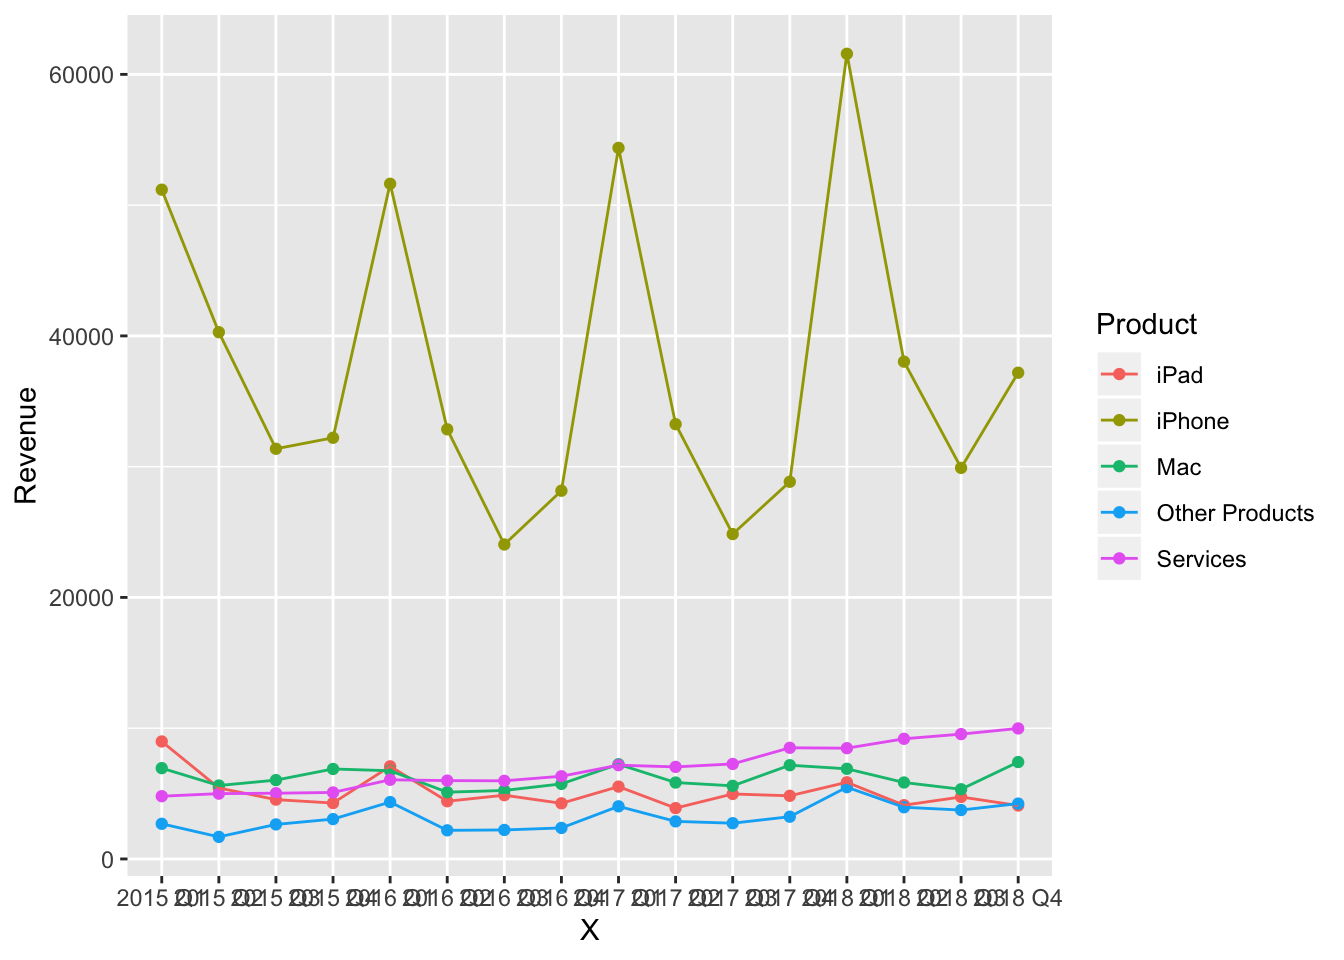
\includegraphics{texts_files/figure-latex/unnamed-chunk-73-1.pdf}

\begin{Shaded}
\begin{Highlighting}[]
\NormalTok{df <-}\StringTok{ }\NormalTok{apple}
\NormalTok{df}\OperatorTok{$}\NormalTok{Quarter =}\StringTok{ }\KeywordTok{paste}\NormalTok{(apple}\OperatorTok{$}\NormalTok{Year, apple}\OperatorTok{$}\NormalTok{Quarter, }\DataTypeTok{sep =} \StringTok{" Q"}\NormalTok{)}
\KeywordTok{head}\NormalTok{(df)}
\end{Highlighting}
\end{Shaded}

\begin{verbatim}
## # A tibble: 6 x 6
##    Year Quarter Product        Units Revenue X      
##   <int> <chr>   <chr>          <dbl>   <dbl> <chr>  
## 1  2015 2015 Q1 iPad           21419    8985 2015 Q1
## 2  2015 2015 Q1 iPhone         74468   51182 2015 Q1
## 3  2015 2015 Q1 Mac             5519    6944 2015 Q1
## 4  2015 2015 Q1 Other Products    NA    2689 2015 Q1
## 5  2015 2015 Q1 Services          NA    4799 2015 Q1
## 6  2015 2015 Q2 iPad           12623    5428 2015 Q2
\end{verbatim}

\begin{Shaded}
\begin{Highlighting}[]
\KeywordTok{qplot}\NormalTok{(}\DataTypeTok{x =}\NormalTok{ Quarter, }\DataTypeTok{y =}\NormalTok{ Revenue, }\DataTypeTok{data =}\NormalTok{ df, }\DataTypeTok{group =}\NormalTok{ Product, }\DataTypeTok{colour =}\NormalTok{ Product, }\DataTypeTok{geom =} \KeywordTok{c}\NormalTok{(}\StringTok{"point"}\NormalTok{, }\StringTok{"line"}\NormalTok{)) }\OperatorTok{+}\StringTok{ }\KeywordTok{theme}\NormalTok{(}\DataTypeTok{axis.text.x =} \KeywordTok{element_text}\NormalTok{(}\DataTypeTok{angle =} \DecValTok{90}\NormalTok{))}
\end{Highlighting}
\end{Shaded}

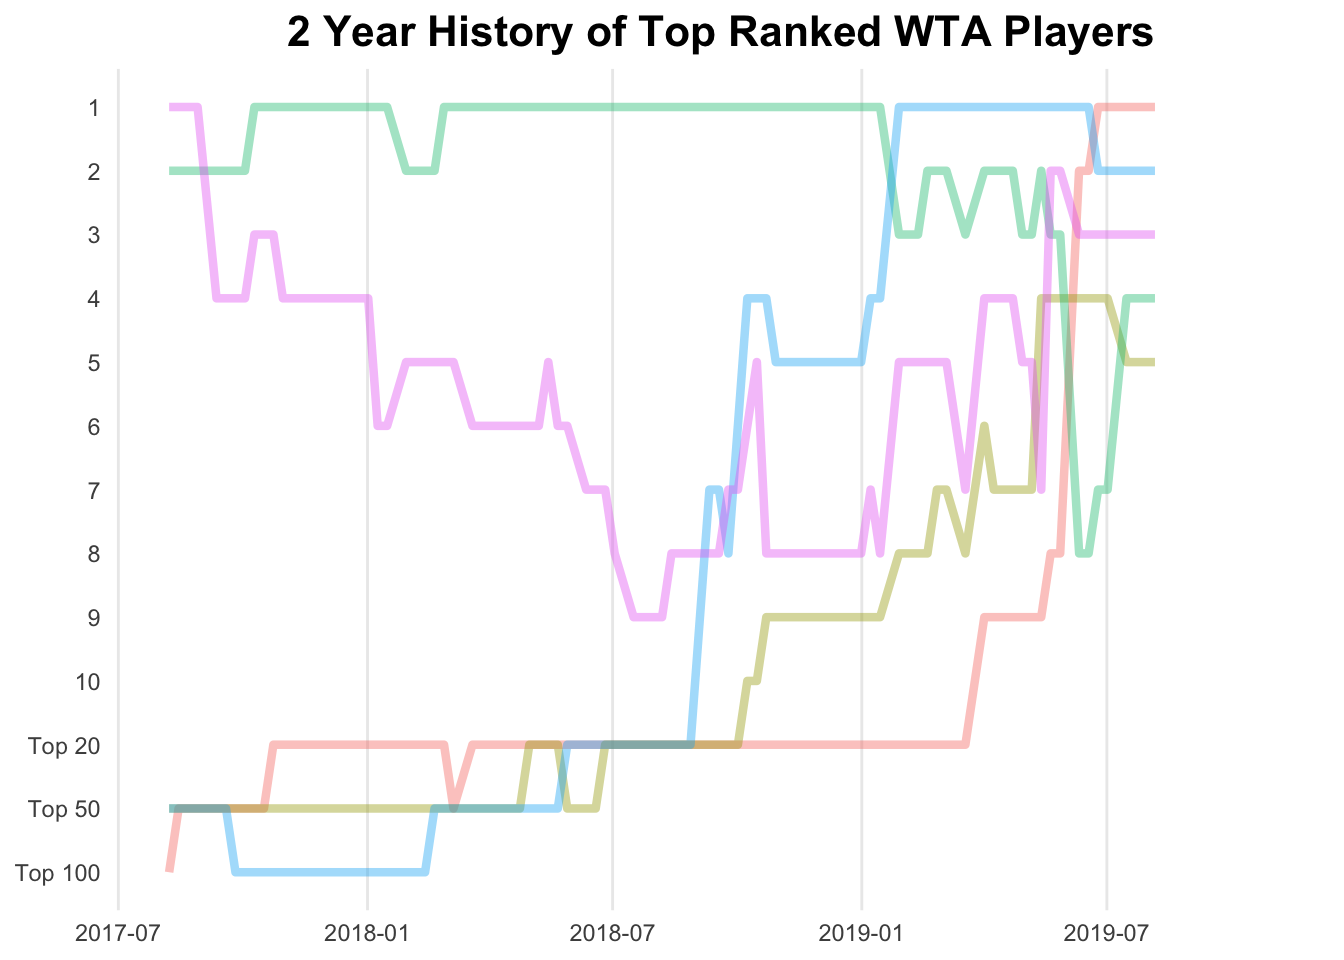
\includegraphics{texts_files/figure-latex/unnamed-chunk-75-1.pdf}

\hypertarget{intro-to-ggplot2}{%
\chapter{Intro to ggplot2}\label{intro-to-ggplot2}}

\begin{Shaded}
\begin{Highlighting}[]
\KeywordTok{library}\NormalTok{(ggplot2)}
\end{Highlighting}
\end{Shaded}

\begin{Shaded}
\begin{Highlighting}[]
\KeywordTok{library}\NormalTok{(scales)}
\end{Highlighting}
\end{Shaded}

\begin{itemize}
\tightlist
\item
  ggplot

  \begin{itemize}
  \tightlist
  \item
    data
  \item
    aesthetic: a mapping
  \end{itemize}
\item
  geometry
\end{itemize}

\hypertarget{ggaes}{%
\section*{aesthetics}\label{ggaes}}
\addcontentsline{toc}{section}{aesthetics}

\begin{itemize}
\tightlist
\item
  x: 1st variable
\item
  y: 2nd variable\\
\item
  group: variable
\item
  colour/color
\end{itemize}

\begin{Shaded}
\begin{Highlighting}[]
\KeywordTok{library}\NormalTok{(dplyr)}
\KeywordTok{library}\NormalTok{(notitia)}
\end{Highlighting}
\end{Shaded}

\hypertarget{gggeoms}{%
\section*{ggplot2 Geometries}\label{gggeoms}}
\addcontentsline{toc}{section}{ggplot2 Geometries}

\hypertarget{geomquant}{%
\section*{Geometries for displaying quantities (or proportions)}\label{geomquant}}
\addcontentsline{toc}{section}{Geometries for displaying quantities (or proportions)}

\hypertarget{geombar}{%
\subsection*{\texorpdfstring{\textbf{geom\_bar}}{geom\_bar}}\label{geombar}}
\addcontentsline{toc}{subsection}{\textbf{geom\_bar}}

\begin{Shaded}
\begin{Highlighting}[]
\NormalTok{chicago <-}\StringTok{ }\NormalTok{chi_emps}
\NormalTok{dept_counts <-}\StringTok{ }\KeywordTok{table}\NormalTok{(chicago}\OperatorTok{$}\NormalTok{Department)}
\NormalTok{dept_counts <-}\StringTok{ }\KeywordTok{sort}\NormalTok{(dept_counts[dept_counts }\OperatorTok{>}\StringTok{ }\DecValTok{1000}\NormalTok{])}
\NormalTok{dept_names <-}\StringTok{ }\KeywordTok{names}\NormalTok{(dept_counts)}
\NormalTok{chicago}\OperatorTok{$}\NormalTok{Dept <-}\StringTok{ }\KeywordTok{ifelse}\NormalTok{(chicago}\OperatorTok{$}\NormalTok{Department }\OperatorTok\StringTok{ }\NormalTok{dept_names, chicago}\OperatorTok{$}\NormalTok{Department, }\StringTok{"OTHER"}\NormalTok{)}
\NormalTok{chicago}\OperatorTok{$}\NormalTok{Dept <-}\StringTok{ }\KeywordTok{factor}\NormalTok{(chicago}\OperatorTok{$}\NormalTok{Dept, }\DataTypeTok{levels =} \KeywordTok{c}\NormalTok{(}\StringTok{"OTHER"}\NormalTok{, dept_names))}


\KeywordTok{ggplot}\NormalTok{(}\DataTypeTok{data =}\NormalTok{ chicago, }\KeywordTok{aes}\NormalTok{(}\DataTypeTok{x =}\NormalTok{ Dept)) }\OperatorTok{+}\StringTok{ }
\StringTok{  }\KeywordTok{geom_bar}\NormalTok{(}\DataTypeTok{fill =} \StringTok{"purple"}\NormalTok{) }\OperatorTok{+}
\StringTok{  }\KeywordTok{coord_flip}\NormalTok{() }\OperatorTok{+}\StringTok{ }\KeywordTok{xlab}\NormalTok{(}\StringTok{""}\NormalTok{) }\OperatorTok{+}\StringTok{ }\KeywordTok{ylab}\NormalTok{(}\StringTok{"Employees"}\NormalTok{)}
\end{Highlighting}
\end{Shaded}

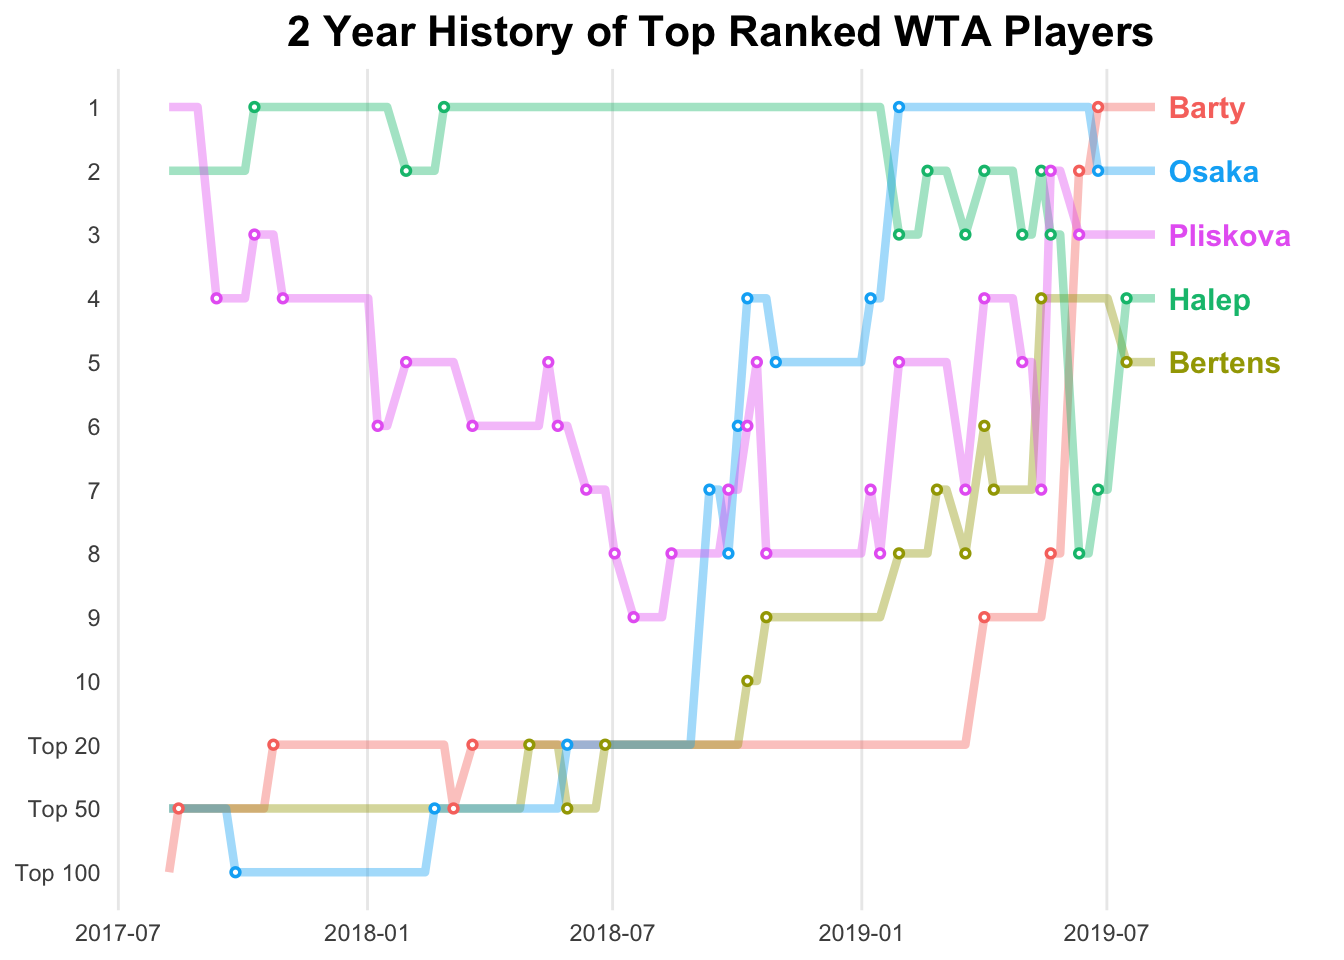
\includegraphics{texts_files/figure-latex/unnamed-chunk-79-1.pdf}

\begin{Shaded}
\begin{Highlighting}[]
\KeywordTok{ggplot}\NormalTok{(rafa_novak, }\KeywordTok{aes}\NormalTok{(}\DataTypeTok{x =}\NormalTok{ Surface, }\DataTypeTok{fill =}\NormalTok{ Winner)) }\OperatorTok{+}\StringTok{ }\KeywordTok{geom_bar}\NormalTok{(}\DataTypeTok{position =} \StringTok{"dodge"}\NormalTok{)}
\end{Highlighting}
\end{Shaded}

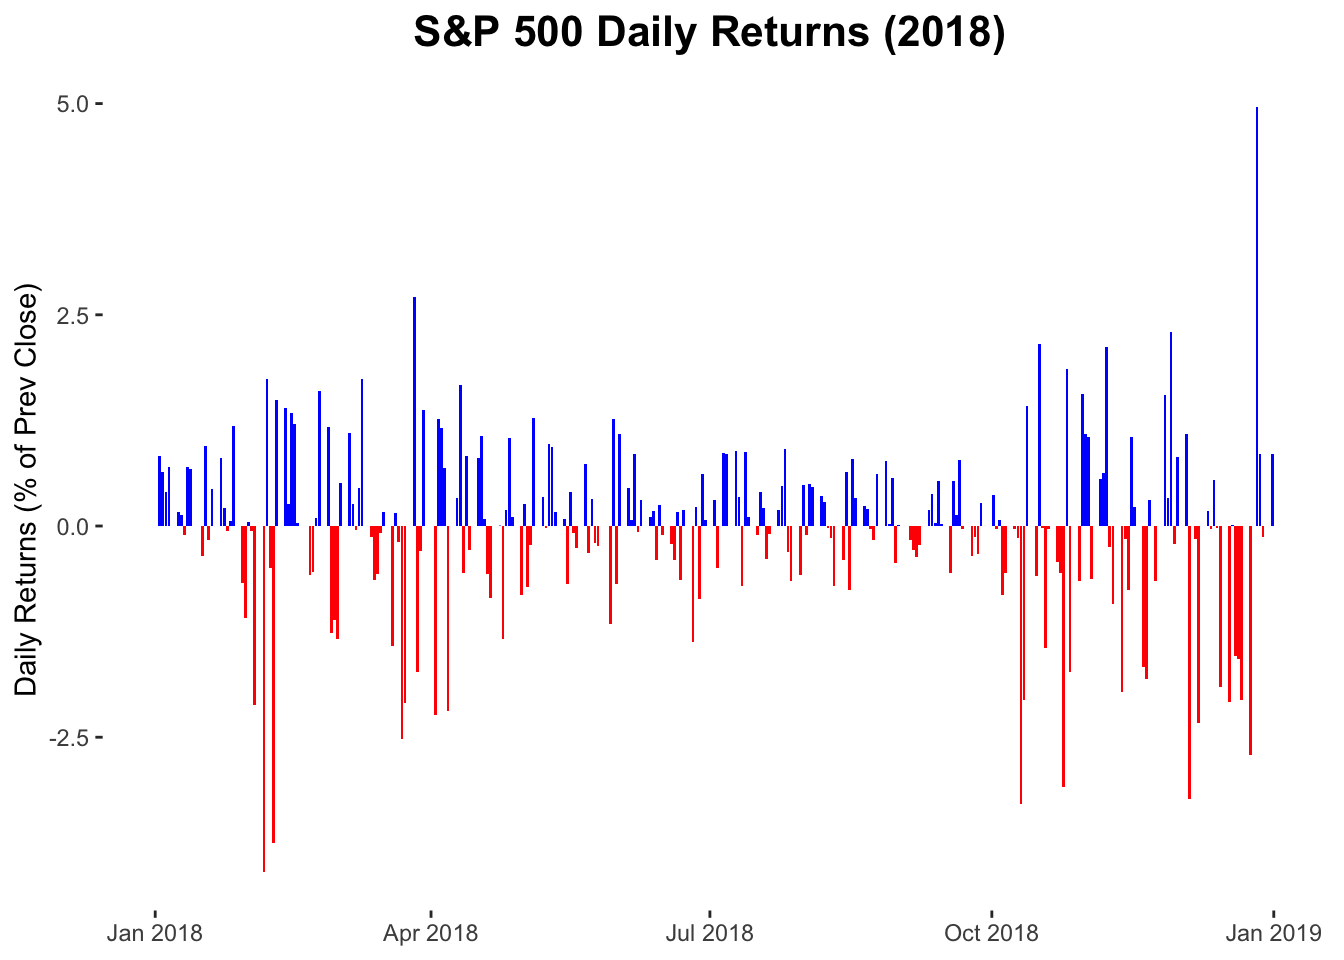
\includegraphics{texts_files/figure-latex/unnamed-chunk-80-1.pdf}

\begin{Shaded}
\begin{Highlighting}[]
\NormalTok{lbj_reg <-}\StringTok{ }\KeywordTok{select}\NormalTok{(lebron, Season, MP) }\OperatorTok\StringTok{ }\KeywordTok{mutate}\NormalTok{(}\DataTypeTok{RegPlayoffs =} \StringTok{"Regular Season"}\NormalTok{)}
\NormalTok{lbj_playoffs <-}\StringTok{ }\KeywordTok{select}\NormalTok{(lebron_playoffs, Season, MP) }\OperatorTok\StringTok{ }\KeywordTok{mutate}\NormalTok{(}\DataTypeTok{RegPlayoffs =} \StringTok{"Playoffs"}\NormalTok{)}
\NormalTok{lbj_mp <-}\StringTok{ }\KeywordTok{bind_rows}\NormalTok{(lbj_reg, lbj_playoffs) }\OperatorTok\StringTok{ }\KeywordTok{filter}\NormalTok{(Season }\OperatorTok{!=}\StringTok{ "Career"}\NormalTok{) }
\NormalTok{lbj_mp_totals <-}\StringTok{ }\KeywordTok{group_by}\NormalTok{(lbj_mp, Season) }\OperatorTok\StringTok{ }\KeywordTok{summarise}\NormalTok{(}\DataTypeTok{MP =} \KeywordTok{sum}\NormalTok{(MP))}


\KeywordTok{ggplot}\NormalTok{(}\DataTypeTok{data =}\NormalTok{ lbj_mp, }\KeywordTok{aes}\NormalTok{(}\DataTypeTok{x =}\NormalTok{ Season, }\DataTypeTok{y =}\NormalTok{ MP)) }\OperatorTok{+}\StringTok{ }
\StringTok{  }\KeywordTok{geom_bar}\NormalTok{(}\DataTypeTok{data =}\NormalTok{ lbj_mp_totals, }\DataTypeTok{colour =} \StringTok{"lightgrey"}\NormalTok{, }\DataTypeTok{stat =} \StringTok{"identity"}\NormalTok{, }\DataTypeTok{alpha =} \FloatTok{.1}\NormalTok{) }\OperatorTok{+}
\StringTok{  }\KeywordTok{geom_bar}\NormalTok{(}\DataTypeTok{stat =} \StringTok{"identity"}\NormalTok{, }\DataTypeTok{mapping =} \KeywordTok{aes}\NormalTok{(}\DataTypeTok{fill =}\NormalTok{ RegPlayoffs)) }\OperatorTok{+}
\StringTok{  }\KeywordTok{guides}\NormalTok{(}\DataTypeTok{fill =} \OtherTok{FALSE}\NormalTok{) }\OperatorTok{+}\StringTok{  }
\StringTok{  }\KeywordTok{facet_wrap}\NormalTok{(}\OperatorTok{~}\StringTok{ }\NormalTok{RegPlayoffs, }\DataTypeTok{ncol =} \DecValTok{1}\NormalTok{) }\OperatorTok{+}
\StringTok{  }\KeywordTok{scale_fill_manual}\NormalTok{(}\DataTypeTok{values =} \KeywordTok{c}\NormalTok{(}\StringTok{"#D9717D"}\NormalTok{, }\StringTok{"#4DB6D0"}\NormalTok{)) }\OperatorTok{+}\StringTok{ }
\StringTok{  }\KeywordTok{theme_bw}\NormalTok{() }
\end{Highlighting}
\end{Shaded}

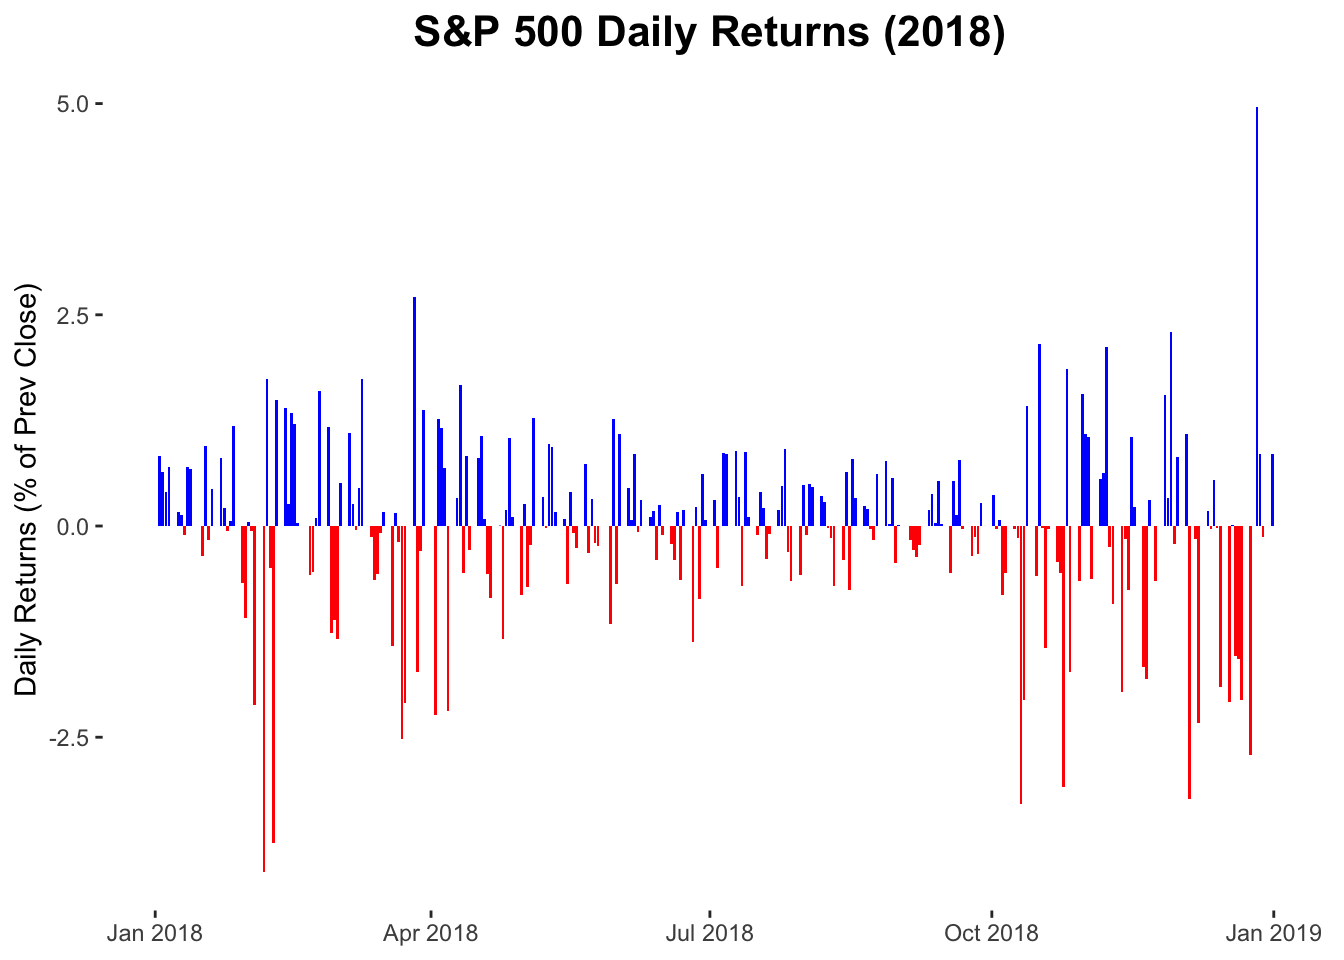
\includegraphics{texts_files/figure-latex/unnamed-chunk-81-1.pdf}

\url{https://michaeltoth.me/a-detailed-guide-to-ggplot-colors.html}

\begin{Shaded}
\begin{Highlighting}[]
\KeywordTok{library}\NormalTok{(tidyr)}
\NormalTok{lbj_reg_min <-}\StringTok{ }\KeywordTok{select}\NormalTok{(lebron, Season, MP) }\OperatorTok\StringTok{ }\KeywordTok{rename}\NormalTok{(}\DataTypeTok{MPR =}\NormalTok{ MP)}
\NormalTok{lbj_playoffs_min <-}\StringTok{ }\KeywordTok{select}\NormalTok{(lebron_playoffs, Season, MP) }\OperatorTok\StringTok{ }\KeywordTok{rename}\NormalTok{(}\DataTypeTok{MPP =}\NormalTok{ MP)}


\NormalTok{lbj_all_min <-}\StringTok{ }\KeywordTok{full_join}\NormalTok{(lbj_reg_min, lbj_playoffs_min, }\DataTypeTok{by =} \StringTok{"Season"}\NormalTok{) }\OperatorTok\StringTok{ }
\StringTok{  }\KeywordTok{filter}\NormalTok{(Season }\OperatorTok{!=}\StringTok{ "Career"}\NormalTok{) }\OperatorTok\StringTok{ }
\StringTok{  }\KeywordTok{mutate}\NormalTok{(}\DataTypeTok{MPR =} \KeywordTok{if_else}\NormalTok{(}\KeywordTok{is.na}\NormalTok{(MPR), }\DecValTok{0}\NormalTok{, MPR), }
         \DataTypeTok{MPP =} \KeywordTok{if_else}\NormalTok{(}\KeywordTok{is.na}\NormalTok{(MPP), }\DecValTok{0}\NormalTok{, MPP),}
         \DataTypeTok{Playoffs =} \KeywordTok{cumsum}\NormalTok{(MPP),}
         \StringTok{`}\DataTypeTok{Reg Season}\StringTok{`}\NormalTok{ =}\StringTok{ }\KeywordTok{cumsum}\NormalTok{(MPR)) }\OperatorTok
\StringTok{  }\KeywordTok{gather}\NormalTok{(}\DataTypeTok{key =}\NormalTok{ RegPlayoffs, }\DataTypeTok{value =}\NormalTok{ MP, Playoffs}\OperatorTok{:}\StringTok{`}\DataTypeTok{Reg Season}\StringTok{`}\NormalTok{) }
\end{Highlighting}
\end{Shaded}

\begin{Shaded}
\begin{Highlighting}[]
\NormalTok{minplot <-}\StringTok{ }\KeywordTok{ggplot}\NormalTok{(}\DataTypeTok{data =}\NormalTok{ lbj_all_min, }\KeywordTok{aes}\NormalTok{(}\DataTypeTok{x =}\NormalTok{ Season, }\DataTypeTok{y =}\NormalTok{ MP, }\DataTypeTok{fill =}\NormalTok{ RegPlayoffs)) }\OperatorTok{+}\StringTok{ }
\StringTok{  }\KeywordTok{geom_bar}\NormalTok{(}\DataTypeTok{stat =} \StringTok{"identity"}\NormalTok{) }\OperatorTok{+}\StringTok{ }
\StringTok{  }\KeywordTok{scale_fill_manual}\NormalTok{(}\DataTypeTok{values =} \KeywordTok{c}\NormalTok{(}\StringTok{"#D9717D"}\NormalTok{, }\StringTok{"#4DB6D0"}\NormalTok{)) }\OperatorTok{+}\StringTok{ }
\StringTok{  }\KeywordTok{theme_bw}\NormalTok{() }\OperatorTok{+}
\StringTok{  }\KeywordTok{geom_segment}\NormalTok{(}\DataTypeTok{x =} \DecValTok{12}\NormalTok{, }\DataTypeTok{xend =} \DecValTok{17}\NormalTok{, }\DataTypeTok{y=}\DecValTok{66297}\NormalTok{, }\DataTypeTok{yend =} \DecValTok{66297}\NormalTok{, }\DataTypeTok{linetype=}\StringTok{"dashed"}\NormalTok{) }\OperatorTok{+}\StringTok{ }\KeywordTok{geom_text}\NormalTok{(}\KeywordTok{aes}\NormalTok{(}\DecValTok{14}\NormalTok{,}\DecValTok{66297}\NormalTok{,}\DataTypeTok{label =} \StringTok{"Kareem Abdul-Jabbar"}\NormalTok{, }\DataTypeTok{vjust =} \DecValTok{-1}\NormalTok{)) }\OperatorTok{+}\StringTok{ }
\StringTok{  }\KeywordTok{geom_segment}\NormalTok{(}\DataTypeTok{x =} \DecValTok{8}\NormalTok{, }\DataTypeTok{xend =} \DecValTok{17}\NormalTok{, }\DataTypeTok{y =} \DecValTok{62759}\NormalTok{, }\DataTypeTok{yend =} \DecValTok{62759}\NormalTok{, }\DataTypeTok{linetype=}\StringTok{"dashed"}\NormalTok{) }\OperatorTok{+}\StringTok{ }\KeywordTok{geom_text}\NormalTok{(}\KeywordTok{aes}\NormalTok{(}\DecValTok{9}\NormalTok{,}\DecValTok{62759}\NormalTok{,}\DataTypeTok{label =} \StringTok{"Karl Malone"}\NormalTok{, }\DataTypeTok{vjust =} \DecValTok{-1}\NormalTok{)) }\OperatorTok{+}
\StringTok{  }\KeywordTok{geom_segment}\NormalTok{(}\DataTypeTok{x =} \DecValTok{5}\NormalTok{, }\DataTypeTok{xend =} \DecValTok{17}\NormalTok{, }\DataTypeTok{y =} \DecValTok{57278}\NormalTok{, }\DataTypeTok{yend =} \DecValTok{57278}\NormalTok{, }\DataTypeTok{linetype=}\StringTok{"dashed"}\NormalTok{) }\OperatorTok{+}\StringTok{ }\KeywordTok{geom_text}\NormalTok{(}\KeywordTok{aes}\NormalTok{(}\DecValTok{6}\NormalTok{,}\DecValTok{57278}\NormalTok{,}\DataTypeTok{label =} \StringTok{"Kobe Bryant"}\NormalTok{, }\DataTypeTok{vjust =} \DecValTok{-1}\NormalTok{)) }\OperatorTok{+}
\StringTok{  }\KeywordTok{geom_segment}\NormalTok{(}\DataTypeTok{x =} \DecValTok{5}\NormalTok{, }\DataTypeTok{xend =} \DecValTok{17}\NormalTok{, }\DataTypeTok{y =} \DecValTok{56738}\NormalTok{, }\DataTypeTok{yend =} \DecValTok{56738}\NormalTok{, }\DataTypeTok{linetype=}\StringTok{"dashed"}\NormalTok{) }\OperatorTok{+}\StringTok{ }\KeywordTok{geom_text}\NormalTok{(}\KeywordTok{aes}\NormalTok{(}\DecValTok{6}\NormalTok{,}\DecValTok{56738}\NormalTok{,}\DataTypeTok{label =} \StringTok{"Tim Duncan"}\NormalTok{, }\DataTypeTok{vjust =} \FloatTok{1.5}\NormalTok{)) }\OperatorTok{+}
\StringTok{  }\KeywordTok{geom_segment}\NormalTok{(}\DataTypeTok{x =} \DecValTok{1}\NormalTok{, }\DataTypeTok{xend =} \DecValTok{17}\NormalTok{, }\DataTypeTok{y =} \DecValTok{50016}\NormalTok{, }\DataTypeTok{yend =} \DecValTok{50016}\NormalTok{, }\DataTypeTok{linetype=}\StringTok{"dashed"}\NormalTok{) }\OperatorTok{+}\StringTok{ }\KeywordTok{geom_text}\NormalTok{(}\KeywordTok{aes}\NormalTok{(}\FloatTok{2.5}\NormalTok{,}\DecValTok{50016}\NormalTok{,}\DataTypeTok{label =} \StringTok{"Shaquille O'Neal"}\NormalTok{, }\DataTypeTok{vjust =} \DecValTok{-1}\NormalTok{)) }\OperatorTok{+}
\StringTok{  }\KeywordTok{geom_segment}\NormalTok{(}\DataTypeTok{x =} \DecValTok{1}\NormalTok{, }\DataTypeTok{xend =} \DecValTok{17}\NormalTok{, }\DataTypeTok{y =} \DecValTok{48485}\NormalTok{, }\DataTypeTok{yend =} \DecValTok{48485}\NormalTok{, }\DataTypeTok{linetype=}\StringTok{"dashed"}\NormalTok{) }\OperatorTok{+}\StringTok{ }\KeywordTok{geom_text}\NormalTok{(}\KeywordTok{aes}\NormalTok{(}\FloatTok{2.4}\NormalTok{,}\DecValTok{48485}\NormalTok{,}\DataTypeTok{label =} \StringTok{"Michael Jordan"}\NormalTok{, }\DataTypeTok{vjust =} \FloatTok{1.5}\NormalTok{)) }\OperatorTok{+}
\StringTok{  }\KeywordTok{geom_segment}\NormalTok{(}\DataTypeTok{x =} \FloatTok{7.2}\NormalTok{, }\DataTypeTok{xend =} \DecValTok{17}\NormalTok{, }\DataTypeTok{y =} \DecValTok{41329}\NormalTok{, }\DataTypeTok{yend =} \DecValTok{41329}\NormalTok{, }\DataTypeTok{linetype=}\StringTok{"dashed"}\NormalTok{) }\OperatorTok{+}\StringTok{ }\KeywordTok{geom_text}\NormalTok{(}\KeywordTok{aes}\NormalTok{(}\DecValTok{8}\NormalTok{,}\DecValTok{41329}\NormalTok{,}\DataTypeTok{label =} \StringTok{"Larry Bird"}\NormalTok{, }\DataTypeTok{vjust =} \DecValTok{-1}\NormalTok{)) }\OperatorTok{+}
\StringTok{   }\KeywordTok{geom_segment}\NormalTok{(}\DataTypeTok{x =} \FloatTok{7.2}\NormalTok{, }\DataTypeTok{xend =} \DecValTok{17}\NormalTok{, }\DataTypeTok{y =} \DecValTok{40783}\NormalTok{, }\DataTypeTok{yend =} \DecValTok{40783}\NormalTok{, }\DataTypeTok{linetype=}\StringTok{"dashed"}\NormalTok{) }\OperatorTok{+}\StringTok{ }\KeywordTok{geom_text}\NormalTok{(}\KeywordTok{aes}\NormalTok{(}\FloatTok{8.5}\NormalTok{,}\DecValTok{40783}\NormalTok{,}\DataTypeTok{label =} \StringTok{"Magic Johnson"}\NormalTok{, }\DataTypeTok{vjust =} \FloatTok{1.5}\NormalTok{)) }\OperatorTok{+}
\StringTok{  }\KeywordTok{scale_y_continuous}\NormalTok{(}\DataTypeTok{label=}\NormalTok{comma, }\DataTypeTok{limits =} \KeywordTok{c}\NormalTok{(}\DecValTok{0}\NormalTok{,}\DecValTok{70000}\NormalTok{)) }\OperatorTok{+}\StringTok{ }
\StringTok{  }\KeywordTok{theme}\NormalTok{(}\DataTypeTok{panel.grid.major =} \KeywordTok{element_blank}\NormalTok{(), }\DataTypeTok{panel.grid.minor =} \KeywordTok{element_blank}\NormalTok{(), }
        \DataTypeTok{axis.text.x =} \KeywordTok{element_text}\NormalTok{(}\DataTypeTok{angle =} \DecValTok{90}\NormalTok{),}
        \DataTypeTok{plot.title =} \KeywordTok{element_text}\NormalTok{(}\DataTypeTok{size =} \DecValTok{21}\NormalTok{, }\DataTypeTok{face =} \StringTok{"bold"}\NormalTok{),}
        \DataTypeTok{legend.title =} \KeywordTok{element_blank}\NormalTok{()}
\NormalTok{        )}\OperatorTok{+}\StringTok{ }
\StringTok{  }\KeywordTok{ylab}\NormalTok{(}\StringTok{"Cumulative Minutes"}\NormalTok{) }\OperatorTok{+}\StringTok{ }
\StringTok{  }\KeywordTok{ggtitle}\NormalTok{(}\StringTok{"LeBron James Career Minutes Played"}\NormalTok{)}

\NormalTok{minplot}
\end{Highlighting}
\end{Shaded}

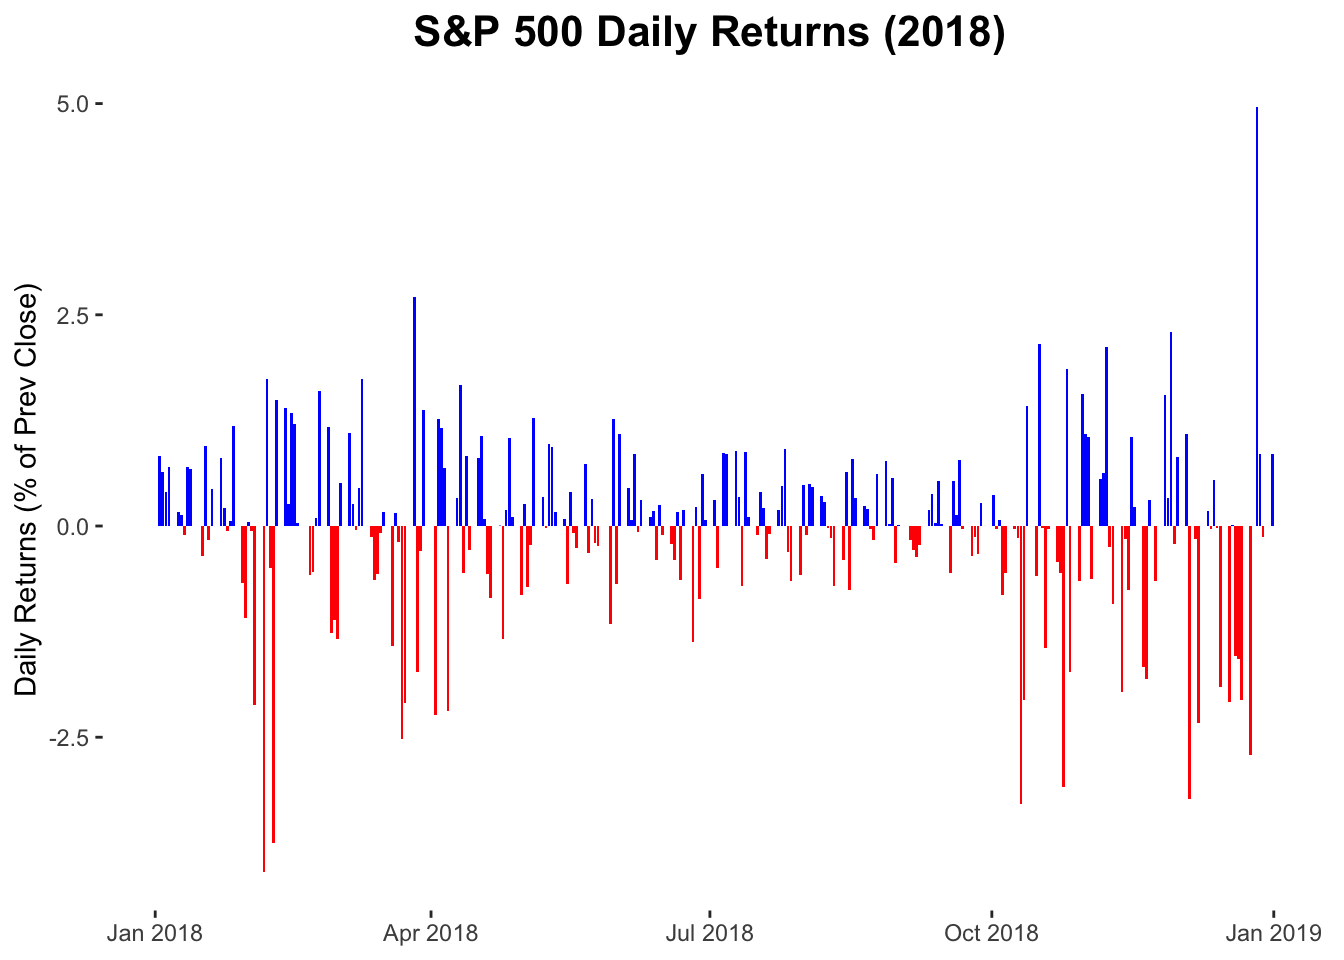
\includegraphics{texts_files/figure-latex/unnamed-chunk-83-1.pdf}

\begin{Shaded}
\begin{Highlighting}[]
\NormalTok{lbj<-}\StringTok{ }\KeywordTok{full_join}\NormalTok{(lbj_reg_min, lbj_playoffs_min, }\DataTypeTok{by =} \StringTok{"Season"}\NormalTok{) }\OperatorTok\StringTok{ }
\StringTok{  }\KeywordTok{filter}\NormalTok{(Season }\OperatorTok{!=}\StringTok{ "Career"}\NormalTok{) }\OperatorTok\StringTok{ }
\StringTok{  }\KeywordTok{mutate}\NormalTok{(}\DataTypeTok{MPR =} \KeywordTok{if_else}\NormalTok{(}\KeywordTok{is.na}\NormalTok{(MPR), }\DecValTok{0}\NormalTok{, MPR), }
         \DataTypeTok{MPP =} \KeywordTok{if_else}\NormalTok{(}\KeywordTok{is.na}\NormalTok{(MPP), }\DecValTok{0}\NormalTok{, MPP),}
         \DataTypeTok{Playoffs =} \KeywordTok{cumsum}\NormalTok{(MPP),}
         \StringTok{`}\DataTypeTok{Reg Season}\StringTok{`}\NormalTok{ =}\StringTok{ }\KeywordTok{cumsum}\NormalTok{(MPR)) }


\NormalTok{minplot2 <-}\StringTok{ }\KeywordTok{ggplot}\NormalTok{(}\DataTypeTok{data =}\NormalTok{ lbj, }\KeywordTok{aes}\NormalTok{(}\DataTypeTok{x =}\NormalTok{ Season)) }\OperatorTok{+}\StringTok{ }
\StringTok{  }\KeywordTok{geom_ribbon}\NormalTok{(}\KeywordTok{aes}\NormalTok{(}\DataTypeTok{ymin =} \DecValTok{0}\NormalTok{, }\DataTypeTok{ymax =} \StringTok{`}\DataTypeTok{Reg Season}\StringTok{`}\NormalTok{, }\DataTypeTok{fill =} \StringTok{"Regular Season"}\NormalTok{), }
              \DataTypeTok{group =} \DecValTok{1}\NormalTok{, }\DataTypeTok{alpha =} \FloatTok{0.6}\NormalTok{) }\OperatorTok{+}\StringTok{ }
\StringTok{  }\KeywordTok{geom_ribbon}\NormalTok{(}\KeywordTok{aes}\NormalTok{(}\DataTypeTok{ymin =} \StringTok{`}\DataTypeTok{Reg Season}\StringTok{`}\NormalTok{, }\DataTypeTok{ymax =} \StringTok{`}\DataTypeTok{Reg Season}\StringTok{`} \OperatorTok{+}\StringTok{ }\NormalTok{Playoffs, }\DataTypeTok{fill =} \StringTok{"Playoffs"}\NormalTok{), }
              \DataTypeTok{group =} \DecValTok{1}\NormalTok{, }\DataTypeTok{alpha =} \FloatTok{0.6}\NormalTok{) }\OperatorTok{+}\StringTok{ }
\StringTok{  }\KeywordTok{theme_bw}\NormalTok{() }\OperatorTok{+}\StringTok{ }
\StringTok{  }\KeywordTok{scale_fill_manual}\NormalTok{(}\DataTypeTok{values =} \KeywordTok{c}\NormalTok{(}\StringTok{"purple"}\NormalTok{, }\StringTok{"blue"}\NormalTok{), }\DataTypeTok{name =} \StringTok{""}\NormalTok{) }\OperatorTok{+}
\StringTok{  }\KeywordTok{theme}\NormalTok{(}\DataTypeTok{panel.grid.major =} \KeywordTok{element_blank}\NormalTok{(), }\DataTypeTok{panel.grid.minor =} \KeywordTok{element_blank}\NormalTok{(), }
        \DataTypeTok{axis.text.x =} \KeywordTok{element_text}\NormalTok{(}\DataTypeTok{angle =} \DecValTok{90}\NormalTok{), }
        \DataTypeTok{plot.title =} \KeywordTok{element_text}\NormalTok{(}\DataTypeTok{size =} \DecValTok{20}\NormalTok{, }\DataTypeTok{face =} \StringTok{"bold"}\NormalTok{)) }\OperatorTok{+}
\StringTok{  }\KeywordTok{ylab}\NormalTok{(}\StringTok{"Cumulative Minutes"}\NormalTok{) }\OperatorTok{+}\StringTok{ }\KeywordTok{scale_y_continuous}\NormalTok{(}\DataTypeTok{label=}\NormalTok{comma, }\DataTypeTok{limits =} \KeywordTok{c}\NormalTok{(}\DecValTok{0}\NormalTok{,}\DecValTok{70000}\NormalTok{)) }\OperatorTok{+}
\StringTok{  }\KeywordTok{geom_hline}\NormalTok{(}\DataTypeTok{yintercept =} \DecValTok{66297}\NormalTok{, }\DataTypeTok{linetype=}\StringTok{"dashed"}\NormalTok{) }\OperatorTok{+}\StringTok{ }
\StringTok{  }\KeywordTok{geom_text}\NormalTok{(}\KeywordTok{aes}\NormalTok{(}\DecValTok{14}\NormalTok{,}\DecValTok{66297}\NormalTok{,}\DataTypeTok{label =} \StringTok{"Kareem Abdul-Jabbar"}\NormalTok{, }\DataTypeTok{vjust =} \DecValTok{-1}\NormalTok{)) }\OperatorTok{+}\StringTok{ }
\StringTok{  }\KeywordTok{geom_hline}\NormalTok{(}\DataTypeTok{yintercept =} \DecValTok{62759}\NormalTok{, }\DataTypeTok{linetype=}\StringTok{"dashed"}\NormalTok{) }\OperatorTok{+}\StringTok{ }
\StringTok{  }\KeywordTok{geom_text}\NormalTok{(}\KeywordTok{aes}\NormalTok{(}\DecValTok{3}\NormalTok{,}\DecValTok{62759}\NormalTok{,}\DataTypeTok{label =} \StringTok{"Karl Malone"}\NormalTok{, }\DataTypeTok{vjust =} \FloatTok{1.5}\NormalTok{)) }\OperatorTok{+}\StringTok{ }
\StringTok{  }\KeywordTok{geom_hline}\NormalTok{(}\DataTypeTok{yintercept =} \DecValTok{57278}\NormalTok{, }\DataTypeTok{linetype=}\StringTok{"dashed"}\NormalTok{) }\OperatorTok{+}\StringTok{ }
\StringTok{  }\KeywordTok{geom_text}\NormalTok{(}\KeywordTok{aes}\NormalTok{(}\DecValTok{14}\NormalTok{,}\DecValTok{57278}\NormalTok{,}\DataTypeTok{label =} \StringTok{"Kobe Bryant"}\NormalTok{, }\DataTypeTok{vjust =} \DecValTok{-1}\NormalTok{)) }\OperatorTok{+}
\StringTok{  }\KeywordTok{geom_hline}\NormalTok{(}\DataTypeTok{yintercept =} \DecValTok{56738}\NormalTok{, }\DataTypeTok{linetype=}\StringTok{"dashed"}\NormalTok{) }\OperatorTok{+}\StringTok{ }
\StringTok{  }\KeywordTok{geom_text}\NormalTok{(}\KeywordTok{aes}\NormalTok{(}\DecValTok{2}\NormalTok{,}\DecValTok{56738}\NormalTok{,}\DataTypeTok{label =} \StringTok{"Tim Duncan"}\NormalTok{, }\DataTypeTok{vjust =} \FloatTok{1.5}\NormalTok{)) }\OperatorTok{+}
\StringTok{  }\KeywordTok{geom_hline}\NormalTok{(}\DataTypeTok{yintercept =} \DecValTok{50016}\NormalTok{, }\DataTypeTok{linetype=}\StringTok{"dashed"}\NormalTok{) }\OperatorTok{+}\StringTok{ }
\StringTok{  }\KeywordTok{geom_text}\NormalTok{(}\KeywordTok{aes}\NormalTok{(}\DecValTok{12}\NormalTok{,}\DecValTok{50016}\NormalTok{,}\DataTypeTok{label =} \StringTok{"Shaquille O'Neal"}\NormalTok{, }\DataTypeTok{vjust =} \DecValTok{-1}\NormalTok{)) }\OperatorTok{+}
\StringTok{  }\KeywordTok{geom_hline}\NormalTok{(}\DataTypeTok{yintercept =} \DecValTok{48485}\NormalTok{, }\DataTypeTok{linetype=}\StringTok{"dashed"}\NormalTok{) }\OperatorTok{+}\StringTok{ }
\StringTok{  }\KeywordTok{geom_text}\NormalTok{(}\KeywordTok{aes}\NormalTok{(}\DecValTok{4}\NormalTok{,}\DecValTok{48485}\NormalTok{,}\DataTypeTok{label =} \StringTok{"Michael Jordan"}\NormalTok{, }\DataTypeTok{vjust =} \FloatTok{1.5}\NormalTok{)) }\OperatorTok{+}
\StringTok{  }\KeywordTok{geom_hline}\NormalTok{(}\DataTypeTok{yintercept =} \DecValTok{41329}\NormalTok{, }\DataTypeTok{linetype=}\StringTok{"dashed"}\NormalTok{) }\OperatorTok{+}\StringTok{ }
\StringTok{  }\KeywordTok{geom_text}\NormalTok{(}\KeywordTok{aes}\NormalTok{(}\DecValTok{10}\NormalTok{,}\DecValTok{41329}\NormalTok{,}\DataTypeTok{label =} \StringTok{"Larry Bird"}\NormalTok{, }\DataTypeTok{vjust =} \DecValTok{-1}\NormalTok{)) }\OperatorTok{+}
\StringTok{  }\KeywordTok{geom_hline}\NormalTok{(}\DataTypeTok{yintercept =} \DecValTok{40783}\NormalTok{, }\DataTypeTok{linetype=}\StringTok{"dashed"}\NormalTok{) }\OperatorTok{+}\StringTok{ }
\StringTok{  }\KeywordTok{geom_text}\NormalTok{(}\KeywordTok{aes}\NormalTok{(}\DecValTok{4}\NormalTok{,}\DecValTok{40783}\NormalTok{,}\DataTypeTok{label =} \StringTok{"Magic Johnson"}\NormalTok{, }\DataTypeTok{vjust =} \FloatTok{1.5}\NormalTok{)) }\OperatorTok{+}\StringTok{ }
\StringTok{  }\KeywordTok{ggtitle}\NormalTok{(}\StringTok{"LeBron James Career Minutes Played"}\NormalTok{)}

\NormalTok{minplot2}
\end{Highlighting}
\end{Shaded}

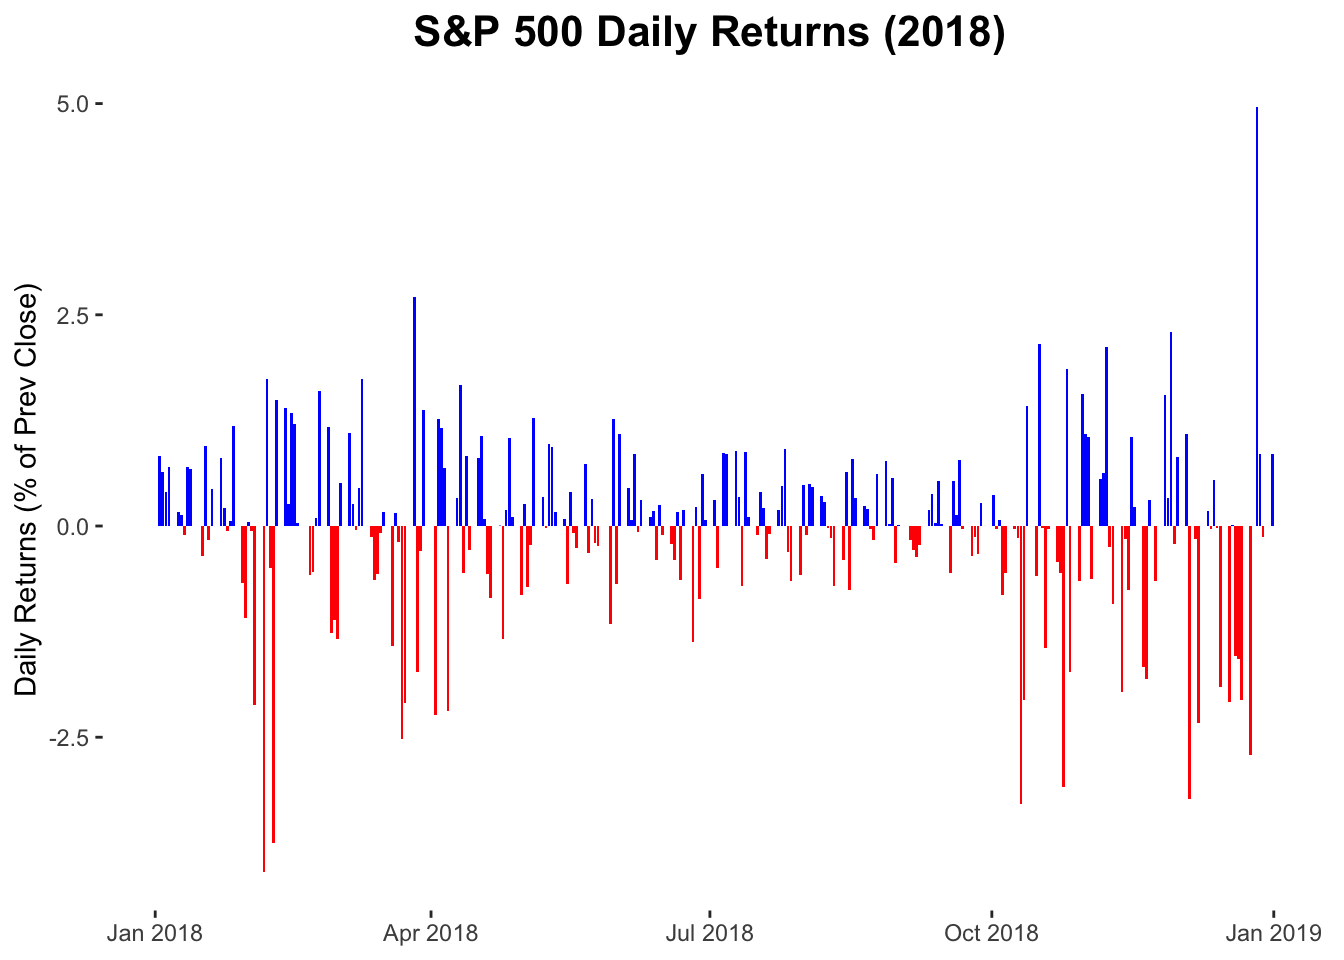
\includegraphics{texts_files/figure-latex/unnamed-chunk-84-1.pdf}

\begin{verbatim}
## Saving 6.5 x 4.5 in image
## Saving 6.5 x 4.5 in image
\end{verbatim}

\hypertarget{xygeom}{%
\section*{Geometries for showing x-y relationships}\label{xygeom}}
\addcontentsline{toc}{section}{Geometries for showing x-y relationships}

\hypertarget{geomscatter}{%
\subsection*{\texorpdfstring{\textbf{geom\_point}: for scatter plots}{geom\_point: for scatter plots}}\label{geomscatter}}
\addcontentsline{toc}{subsection}{\textbf{geom\_point}: for scatter plots}

\begin{Shaded}
\begin{Highlighting}[]
\KeywordTok{ggplot}\NormalTok{(}\DataTypeTok{data =}\NormalTok{ iris, }\KeywordTok{aes}\NormalTok{(}\DataTypeTok{x =}\NormalTok{ Petal.Width, }\DataTypeTok{y =}\NormalTok{ Petal.Length, }\DataTypeTok{colour =}\NormalTok{ Species)) }\OperatorTok{+}\StringTok{ }
\StringTok{  }\KeywordTok{geom_point}\NormalTok{()}
\end{Highlighting}
\end{Shaded}

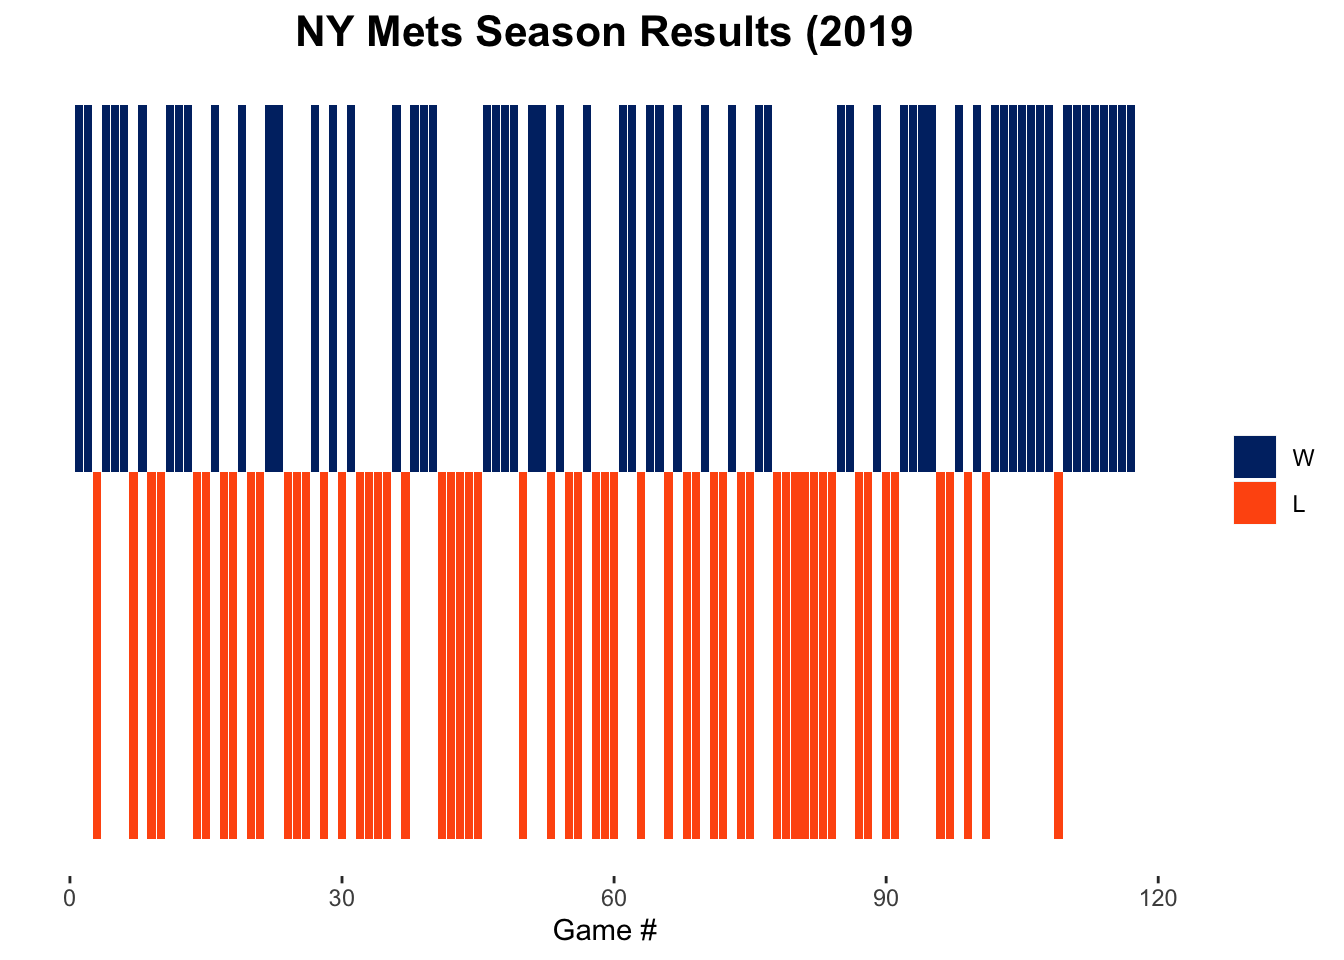
\includegraphics{texts_files/figure-latex/unnamed-chunk-86-1.pdf}

\hypertarget{geomline}{%
\subsection*{\texorpdfstring{\textbf{geom\_line}: for line charts}{geom\_line: for line charts}}\label{geomline}}
\addcontentsline{toc}{subsection}{\textbf{geom\_line}: for line charts}

\begin{Shaded}
\begin{Highlighting}[]
\NormalTok{group_ex <-}\StringTok{ }\NormalTok{life_ex }\OperatorTok\StringTok{ }\KeywordTok{filter}\NormalTok{(}\KeywordTok{grepl}\NormalTok{(}\StringTok{"income countries"}\NormalTok{, Entity)) }

\KeywordTok{ggplot}\NormalTok{(}\DataTypeTok{data =}\NormalTok{ group_ex, }\KeywordTok{aes}\NormalTok{(}\DataTypeTok{x =}\NormalTok{ Year, }\DataTypeTok{y =}\NormalTok{ LE, }\DataTypeTok{group =}\NormalTok{ Entity, }\DataTypeTok{colour =}\NormalTok{ Entity)) }\OperatorTok{+}
\StringTok{  }\KeywordTok{geom_line}\NormalTok{()}
\end{Highlighting}
\end{Shaded}

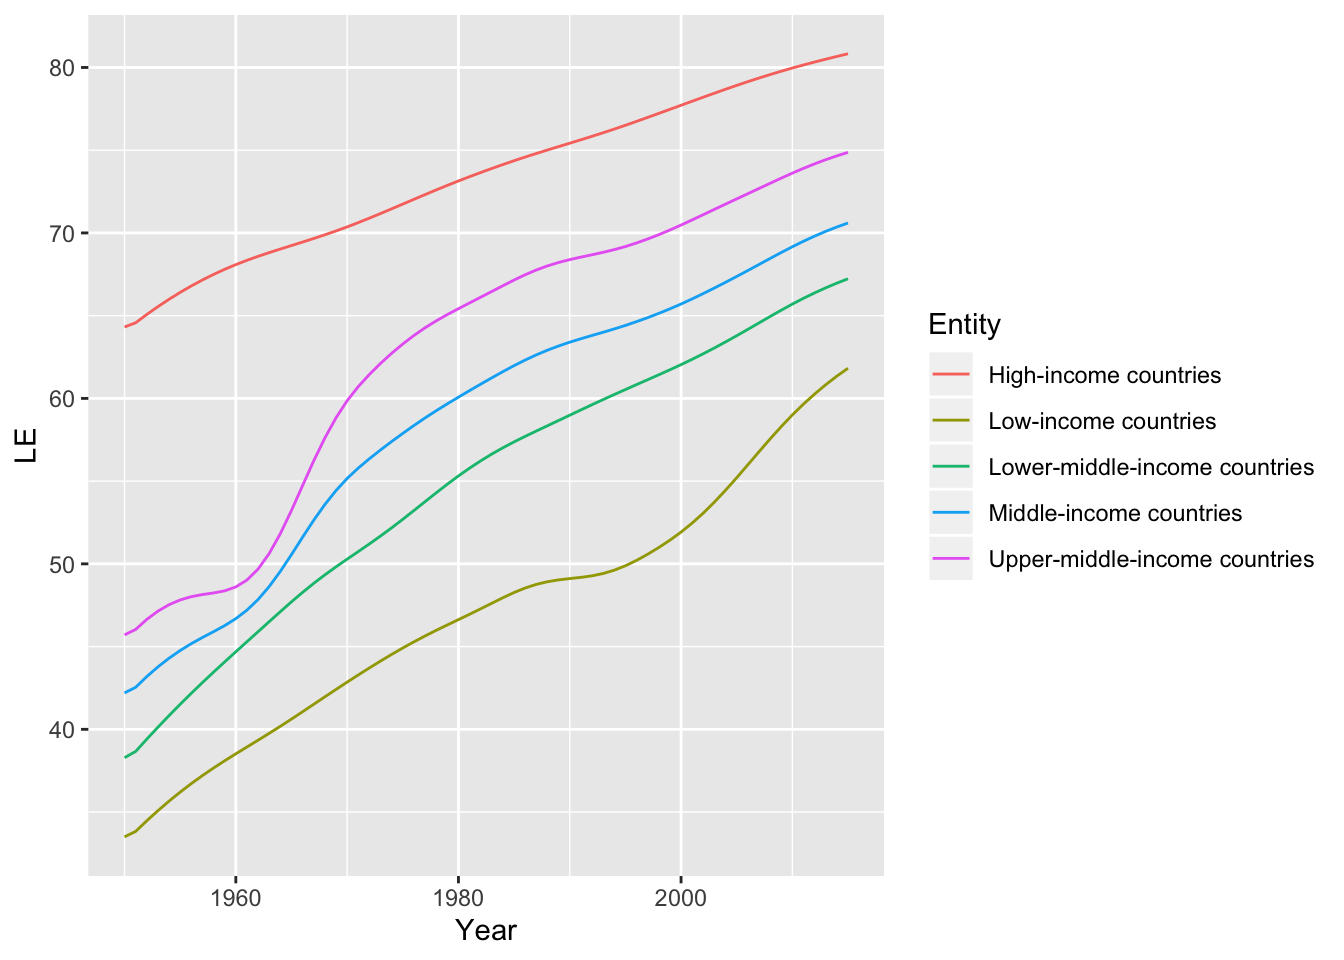
\includegraphics{texts_files/figure-latex/unnamed-chunk-87-1.pdf}

\begin{Shaded}
\begin{Highlighting}[]
\KeywordTok{ggplot}\NormalTok{(}\DataTypeTok{data =}\NormalTok{ apple, }\KeywordTok{aes}\NormalTok{(}\DataTypeTok{x =} \KeywordTok{paste}\NormalTok{(Year, Quarter), }\DataTypeTok{y =}\NormalTok{ Revenue, }\DataTypeTok{group =}\NormalTok{ Product, }\DataTypeTok{colour =}\NormalTok{ Product)) }\OperatorTok{+}\StringTok{ }
\StringTok{  }\KeywordTok{geom_point}\NormalTok{() }\OperatorTok{+}
\StringTok{  }\KeywordTok{geom_line}\NormalTok{()}
\end{Highlighting}
\end{Shaded}

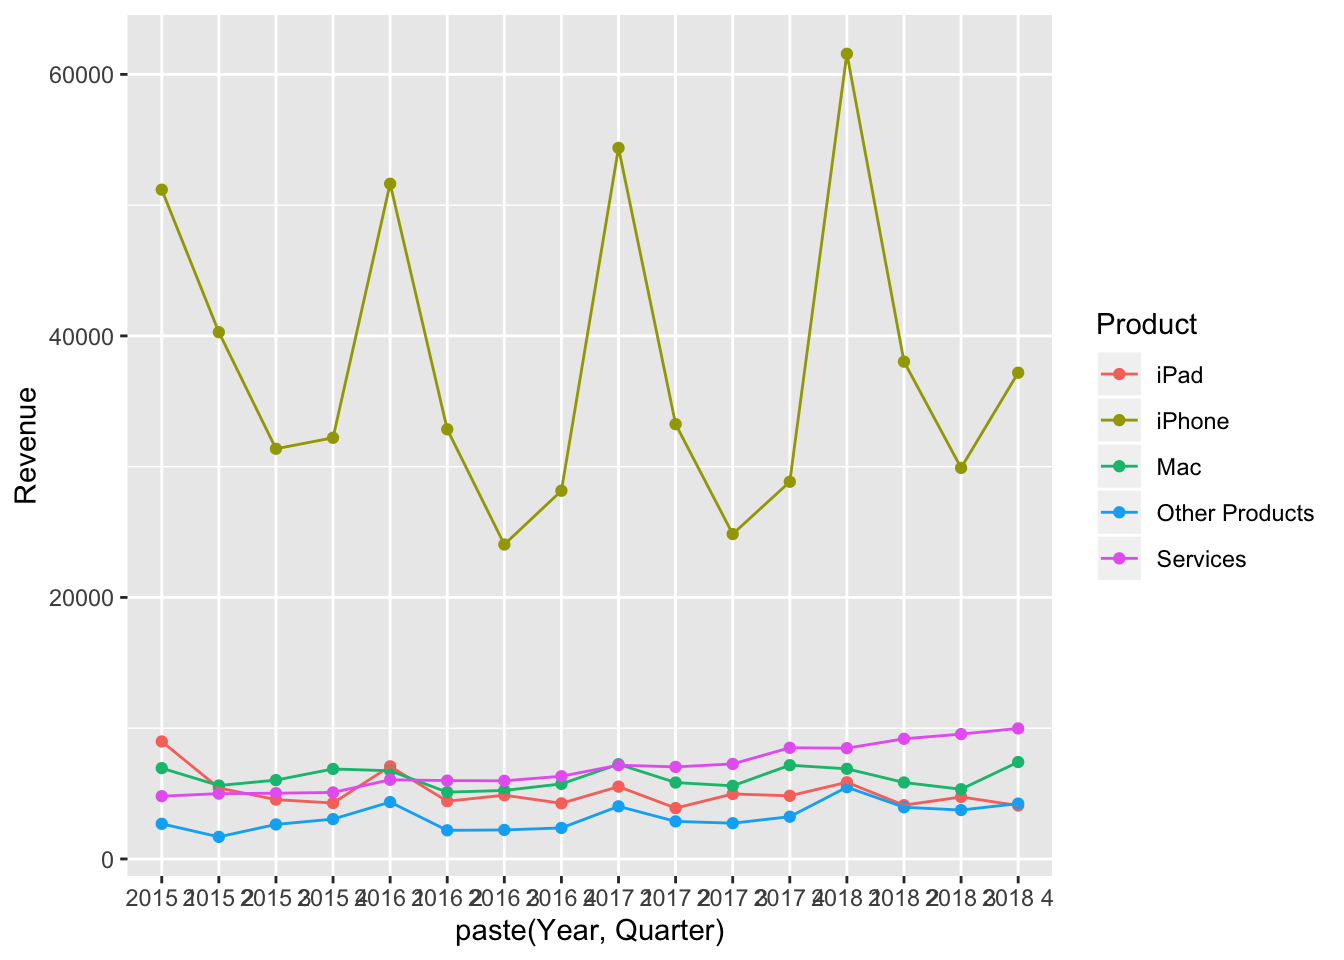
\includegraphics{texts_files/figure-latex/unnamed-chunk-88-1.pdf}

\hypertarget{geomdist}{%
\section*{Geometries for showing distributions}\label{geomdist}}
\addcontentsline{toc}{section}{Geometries for showing distributions}

\hypertarget{geomhistogram}{%
\subsection*{\texorpdfstring{\textbf{geom\_histogram}: for histograms}{geom\_histogram: for histograms}}\label{geomhistogram}}
\addcontentsline{toc}{subsection}{\textbf{geom\_histogram}: for histograms}

\begin{Shaded}
\begin{Highlighting}[]
\KeywordTok{ggplot}\NormalTok{(}\DataTypeTok{data =}\NormalTok{ chi_emps, }\KeywordTok{aes}\NormalTok{(}\DataTypeTok{x =}\NormalTok{ AnnualSalary)) }\OperatorTok{+}\StringTok{ }
\StringTok{  }\KeywordTok{geom_histogram}\NormalTok{(}\DataTypeTok{fill =} \KeywordTok{I}\NormalTok{(}\StringTok{"royalblue"}\NormalTok{), }\DataTypeTok{colour =} \KeywordTok{I}\NormalTok{(}\StringTok{"black"}\NormalTok{))}
\end{Highlighting}
\end{Shaded}

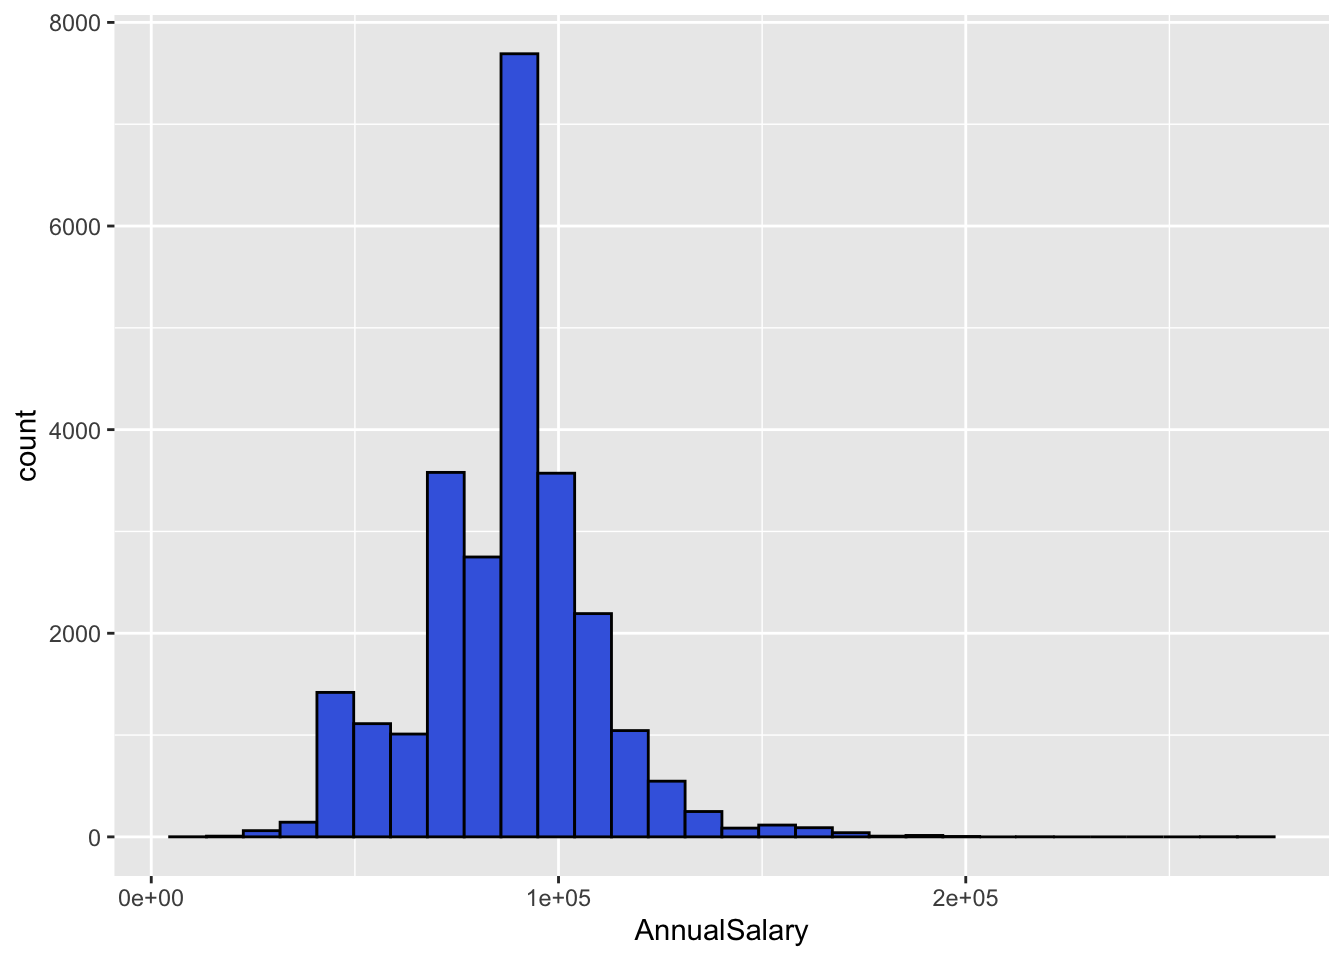
\includegraphics{texts_files/figure-latex/unnamed-chunk-89-1.pdf}

\begin{Shaded}
\begin{Highlighting}[]
\KeywordTok{library}\NormalTok{(NHANES)}
\NormalTok{NHANES_bg <-}\StringTok{ }\KeywordTok{select}\NormalTok{(NHANES, }\OperatorTok{-}\NormalTok{Gender) }\OperatorTok\StringTok{ }
\StringTok{  }\KeywordTok{filter}\NormalTok{(Age }\OperatorTok{>=}\StringTok{ }\DecValTok{18}\NormalTok{)}


\KeywordTok{ggplot}\NormalTok{(}\DataTypeTok{data =}\NormalTok{ NHANES, }\KeywordTok{aes}\NormalTok{(}\DataTypeTok{x =}\NormalTok{ Height)) }\OperatorTok{+}
\StringTok{  }\KeywordTok{geom_histogram}\NormalTok{(}\DataTypeTok{data =}\NormalTok{ NHANES_bg, }\DataTypeTok{fill =} \StringTok{"grey"}\NormalTok{, }\DataTypeTok{alpha =} \FloatTok{.4}\NormalTok{) }\OperatorTok{+}
\StringTok{  }\KeywordTok{geom_histogram}\NormalTok{(}\DataTypeTok{mapping =} \KeywordTok{aes}\NormalTok{(}\DataTypeTok{fill =}\NormalTok{ Gender), }\DataTypeTok{colour =} \StringTok{"black"}\NormalTok{) }\OperatorTok{+}
\StringTok{  }\KeywordTok{facet_wrap}\NormalTok{(}\OperatorTok{~}\StringTok{ }\NormalTok{Gender, }\DataTypeTok{ncol =} \DecValTok{1}\NormalTok{) }\OperatorTok{+}
\StringTok{  }\KeywordTok{guides}\NormalTok{(}\DataTypeTok{fill =} \OtherTok{FALSE}\NormalTok{) }\OperatorTok{+}\StringTok{  }\CommentTok{# to remove the legend}
\StringTok{  }\KeywordTok{theme_bw}\NormalTok{()    }
\end{Highlighting}
\end{Shaded}

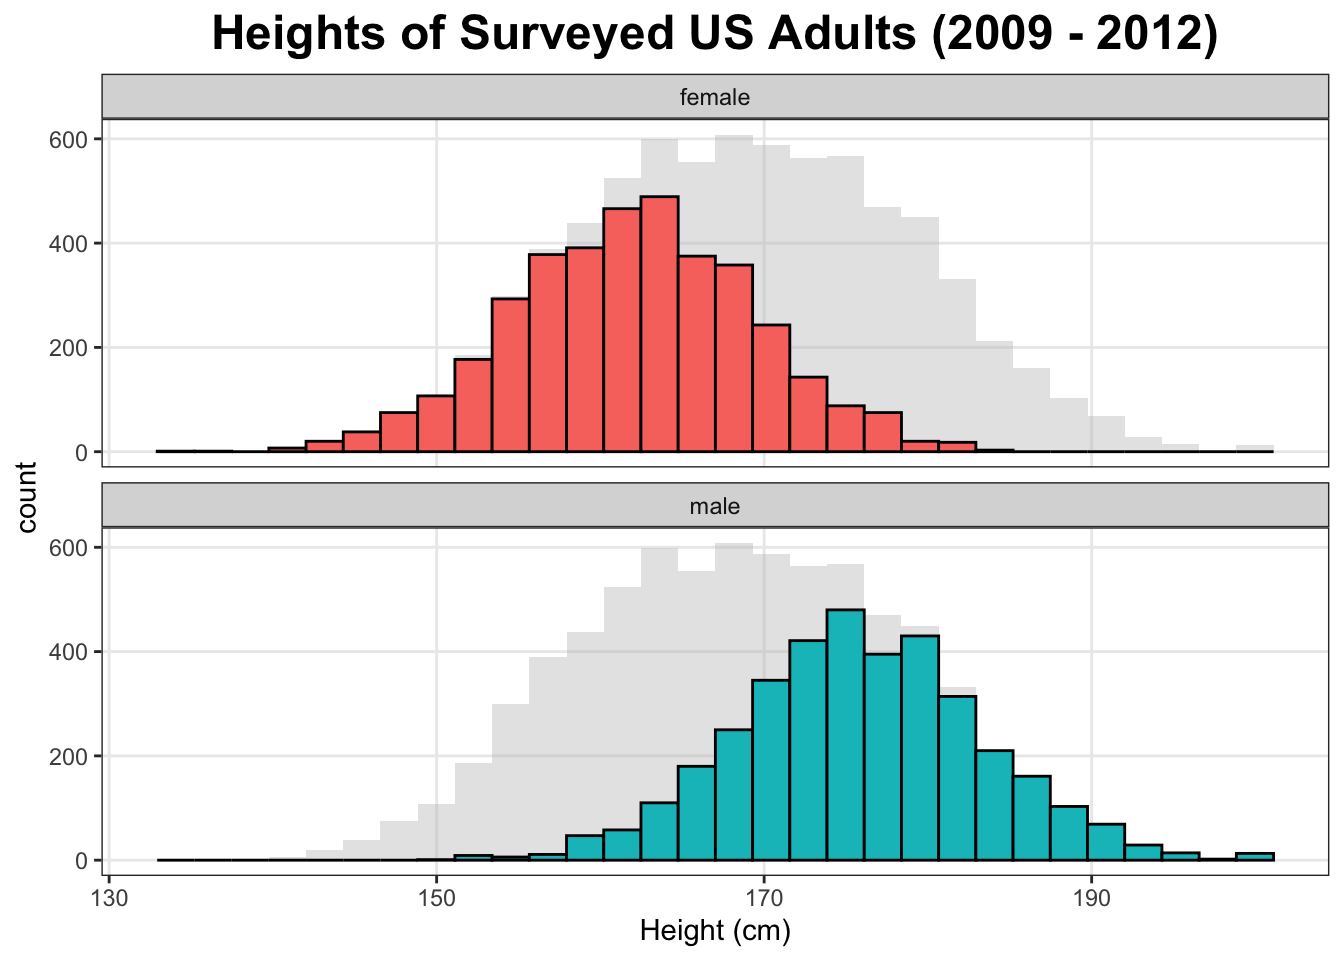
\includegraphics{texts_files/figure-latex/nhaneshists-1.pdf}

\hypertarget{geomboxplot}{%
\subsection*{\texorpdfstring{\textbf{geom\_boxplot}: for boxplots}{geom\_boxplot: for boxplots}}\label{geomboxplot}}
\addcontentsline{toc}{subsection}{\textbf{geom\_boxplot}: for boxplots}

\begin{Shaded}
\begin{Highlighting}[]
\NormalTok{large_dept <-}\StringTok{ }\NormalTok{chi_emps[chi_emps}\OperatorTok{$}\NormalTok{Department }\OperatorTok\StringTok{ }\KeywordTok{c}\NormalTok{(}\StringTok{"POLICE"}\NormalTok{, }\StringTok{"FIRE"}\NormalTok{, }\StringTok{"STREETS & SAN"}\NormalTok{), ]}
\KeywordTok{ggplot}\NormalTok{(}\DataTypeTok{data =}\NormalTok{ large_dept, }\KeywordTok{aes}\NormalTok{(}\DataTypeTok{x =}\NormalTok{ Department, }\DataTypeTok{y =}\NormalTok{ AnnualSalary)) }\OperatorTok{+}\StringTok{ }
\StringTok{  }\KeywordTok{geom_boxplot}\NormalTok{()}
\end{Highlighting}
\end{Shaded}

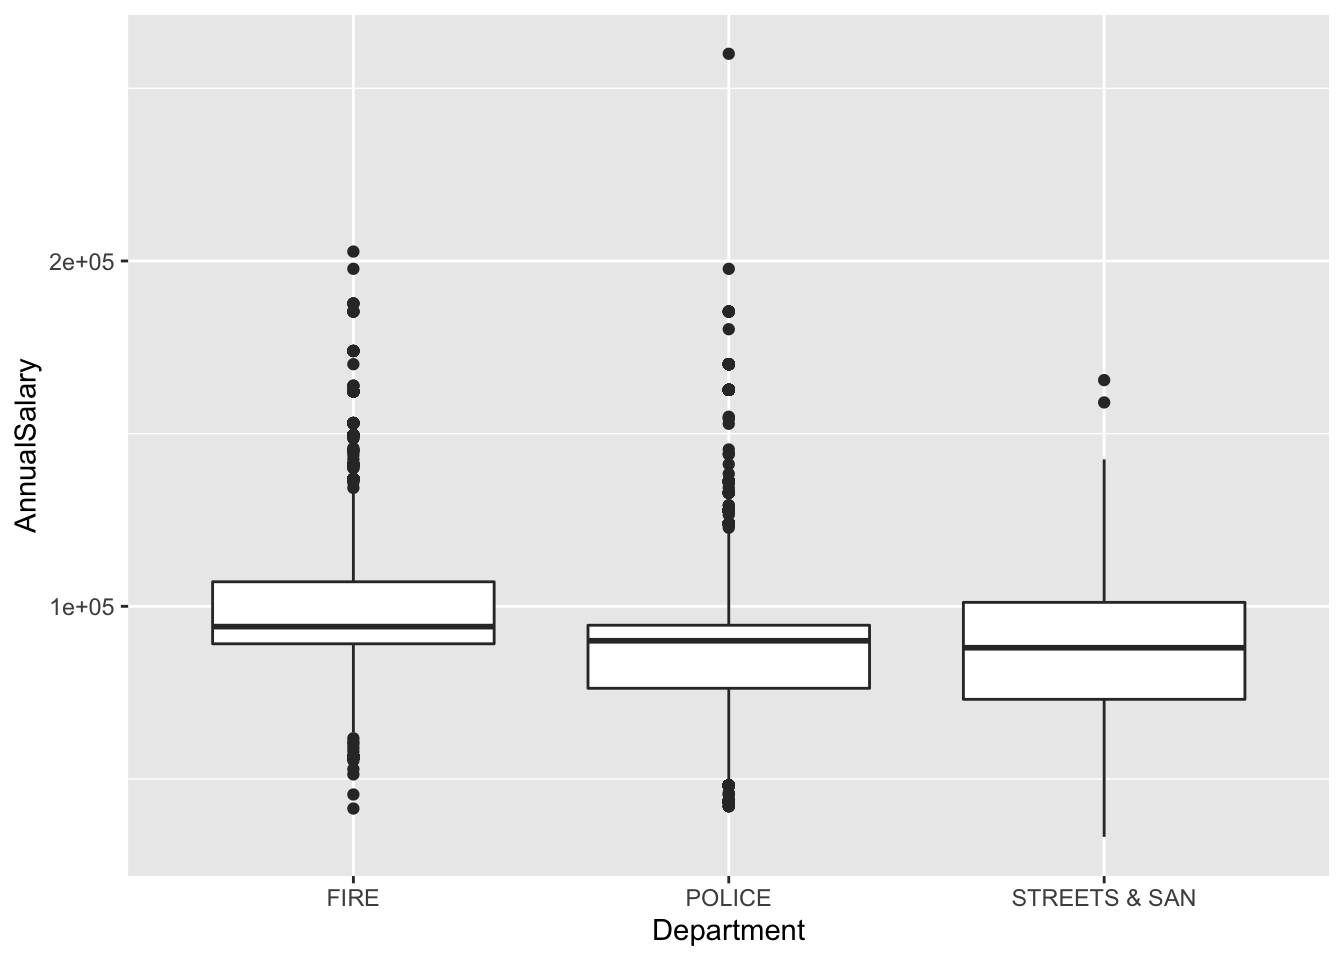
\includegraphics{texts_files/figure-latex/unnamed-chunk-90-1.pdf}

\hypertarget{geomdensity}{%
\subsection*{\texorpdfstring{\textbf{geom\_density}: for density plots}{geom\_density: for density plots}}\label{geomdensity}}
\addcontentsline{toc}{subsection}{\textbf{geom\_density}: for density plots}

\begin{Shaded}
\begin{Highlighting}[]
\KeywordTok{ggplot}\NormalTok{(}\DataTypeTok{data =}\NormalTok{ chicago, }\KeywordTok{aes}\NormalTok{(}\DataTypeTok{x =}\NormalTok{ AnnualSalary)) }\OperatorTok{+}\StringTok{ }\KeywordTok{geom_density}\NormalTok{() }
\end{Highlighting}
\end{Shaded}

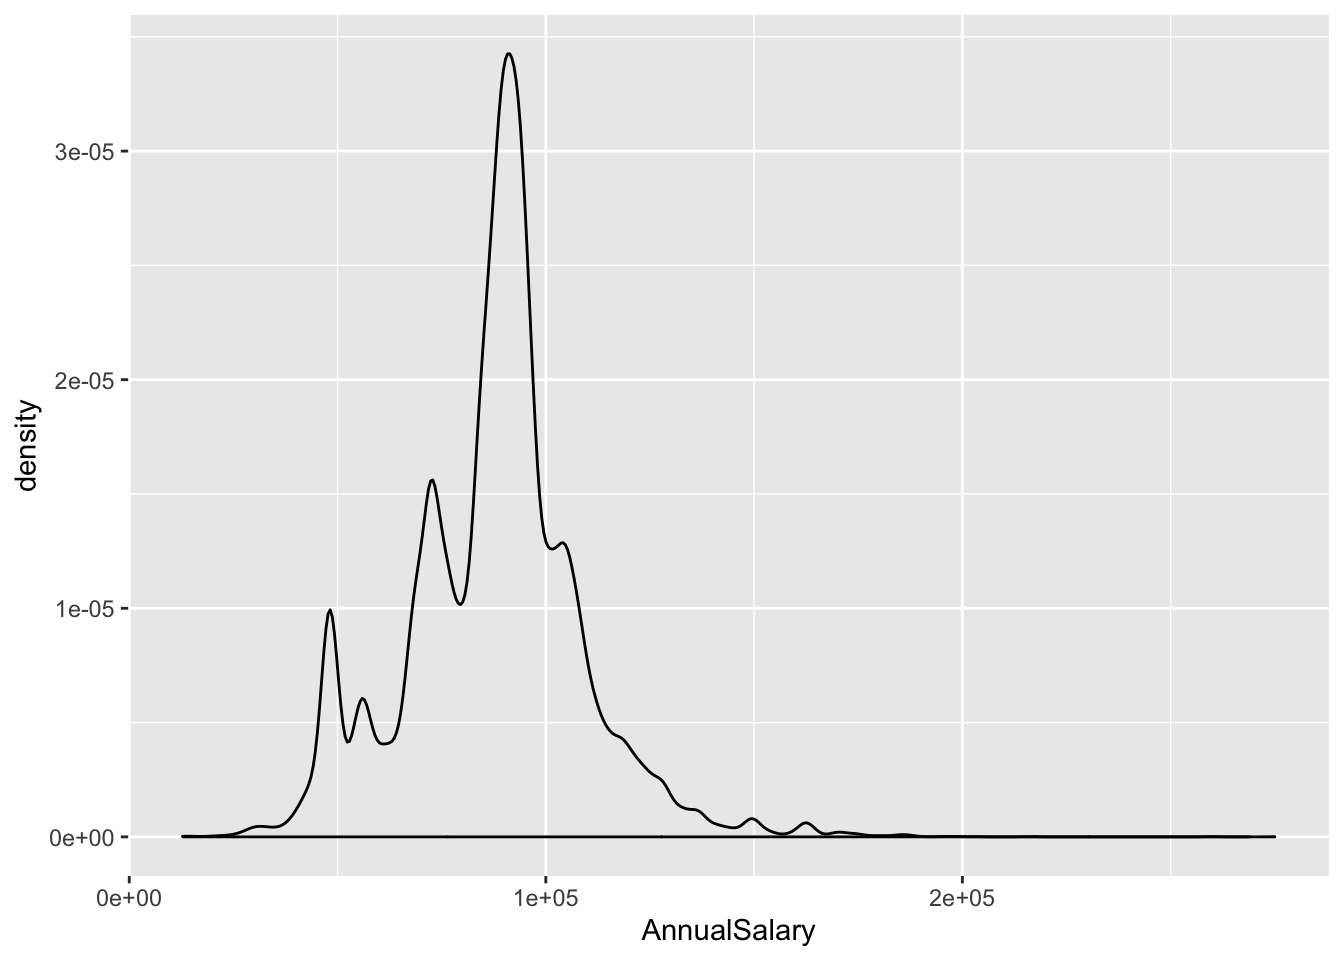
\includegraphics{texts_files/figure-latex/unnamed-chunk-91-1.pdf}

\hypertarget{geomdensityridges}{%
\subsection*{\texorpdfstring{\textbf{geom\_density\_ridges}: for density plots}{geom\_density\_ridges: for density plots}}\label{geomdensityridges}}
\addcontentsline{toc}{subsection}{\textbf{geom\_density\_ridges}: for density plots}

\begin{Shaded}
\begin{Highlighting}[]
\KeywordTok{library}\NormalTok{(ggridges)}

\KeywordTok{ggplot}\NormalTok{(}\DataTypeTok{data =}\NormalTok{ chicago, }\KeywordTok{aes}\NormalTok{(}\DataTypeTok{x =}\NormalTok{ AnnualSalary, }\DataTypeTok{y =}\NormalTok{ Dept)) }\OperatorTok{+}\StringTok{ }
\StringTok{  }\KeywordTok{geom_density_ridges}\NormalTok{() }\OperatorTok{+}\StringTok{ }
\StringTok{  }\KeywordTok{scale_x_continuous}\NormalTok{(}\DataTypeTok{label=}\NormalTok{comma)}
\end{Highlighting}
\end{Shaded}

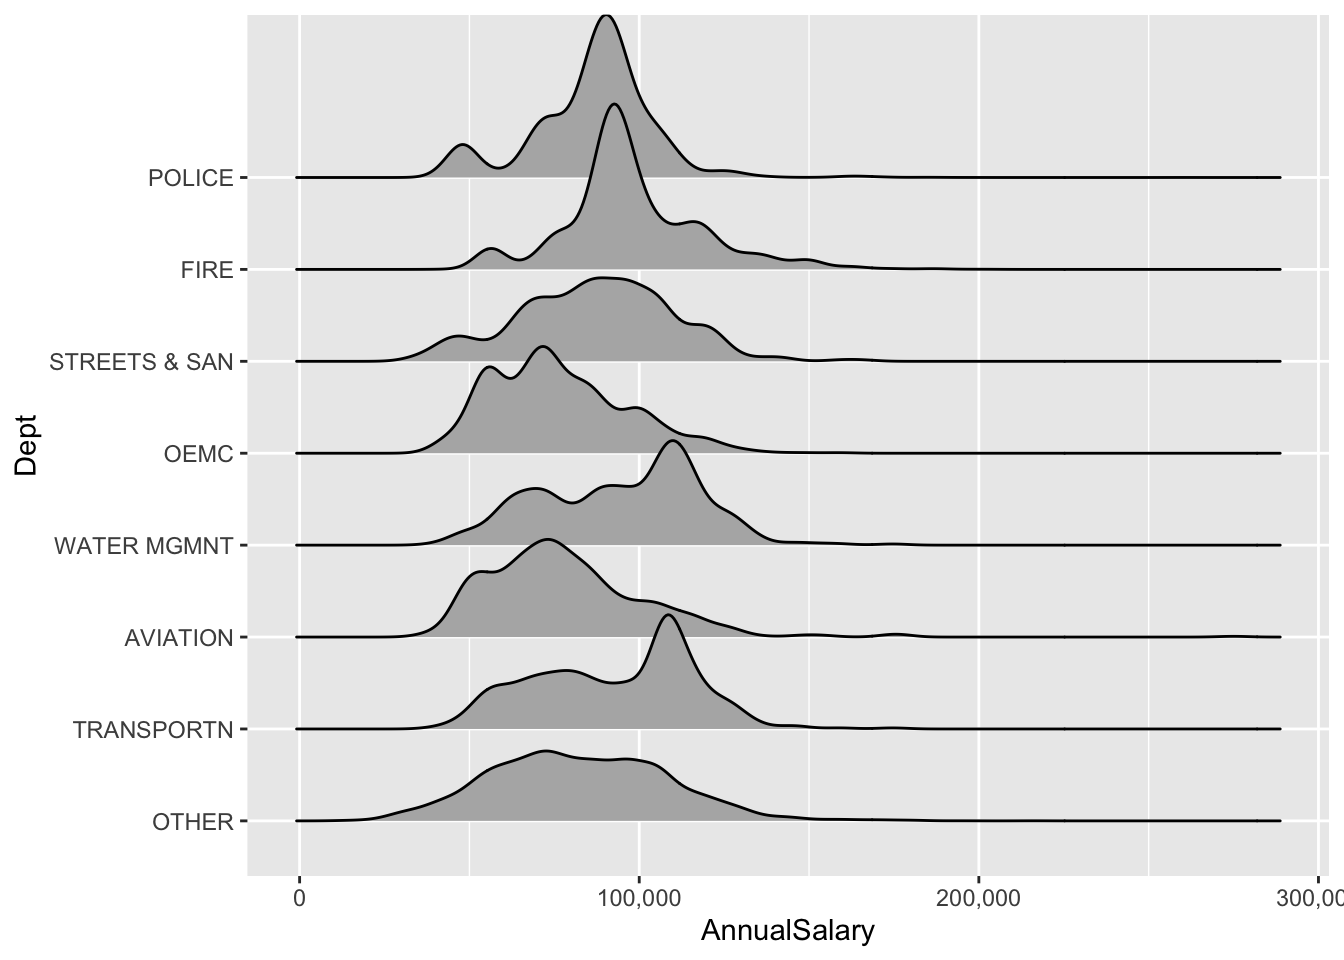
\includegraphics{texts_files/figure-latex/unnamed-chunk-92-1.pdf}

\hypertarget{dplyr-joins}{%
\chapter{dplyr joins}\label{dplyr-joins}}

\begin{Shaded}
\begin{Highlighting}[]
\KeywordTok{library}\NormalTok{(notitia)}
\end{Highlighting}
\end{Shaded}

\begin{Shaded}
\begin{Highlighting}[]
\NormalTok{areas}
\end{Highlighting}
\end{Shaded}

\begin{verbatim}
## # A tibble: 7 x 2
##   country        area
##   <chr>         <dbl>
## 1 Russia        16376
## 2 China          9388
## 3 United States  9147
## 4 Brazil         8358
## 5 India          2973
## 6 Indonesia      1811
## 7 Nigeria         910
\end{verbatim}

\begin{Shaded}
\begin{Highlighting}[]
\NormalTok{populations}
\end{Highlighting}
\end{Shaded}

\begin{verbatim}
## # A tibble: 8 x 2
##   country         pop
##   <chr>         <dbl>
## 1 India          1311
## 2 United States   331
## 3 Indonesia       264
## 4 Pakistan        210
## 5 Nigeria         208
## 6 Bangladesh      161
## 7 Russia          141
## 8 Mexico          127
\end{verbatim}

\begin{Shaded}
\begin{Highlighting}[]
\KeywordTok{library}\NormalTok{(dplyr)}
\end{Highlighting}
\end{Shaded}

\hypertarget{fulljoin}{%
\section*{\texorpdfstring{\textbf{full\_join}}{full\_join}}\label{fulljoin}}
\addcontentsline{toc}{section}{\textbf{full\_join}}

\begin{Shaded}
\begin{Highlighting}[]
\NormalTok{country_info <-}\StringTok{ }\KeywordTok{full_join}\NormalTok{(areas, populations)}
\end{Highlighting}
\end{Shaded}

\begin{verbatim}
## Joining, by = "country"
\end{verbatim}

\begin{Shaded}
\begin{Highlighting}[]
\NormalTok{country_info}
\end{Highlighting}
\end{Shaded}

\begin{verbatim}
## # A tibble: 10 x 3
##    country        area   pop
##    <chr>         <dbl> <dbl>
##  1 Russia        16376   141
##  2 China          9388    NA
##  3 United States  9147   331
##  4 Brazil         8358    NA
##  5 India          2973  1311
##  6 Indonesia      1811   264
##  7 Nigeria         910   208
##  8 Pakistan         NA   210
##  9 Bangladesh       NA   161
## 10 Mexico           NA   127
\end{verbatim}

\hypertarget{innerjoin}{%
\section*{\texorpdfstring{\textbf{inner\_join}}{inner\_join}}\label{innerjoin}}
\addcontentsline{toc}{section}{\textbf{inner\_join}}

\begin{Shaded}
\begin{Highlighting}[]
\NormalTok{country_info <-}\StringTok{ }\KeywordTok{inner_join}\NormalTok{(areas, populations)}
\end{Highlighting}
\end{Shaded}

\begin{verbatim}
## Joining, by = "country"
\end{verbatim}

\begin{Shaded}
\begin{Highlighting}[]
\NormalTok{country_info}
\end{Highlighting}
\end{Shaded}

\begin{verbatim}
## # A tibble: 5 x 3
##   country        area   pop
##   <chr>         <dbl> <dbl>
## 1 Russia        16376   141
## 2 United States  9147   331
## 3 India          2973  1311
## 4 Indonesia      1811   264
## 5 Nigeria         910   208
\end{verbatim}

\hypertarget{leftrightjoin}{%
\section*{\texorpdfstring{\textbf{left\_join} and \textbf{right\_join}}{left\_join and right\_join}}\label{leftrightjoin}}
\addcontentsline{toc}{section}{\textbf{left\_join} and \textbf{right\_join}}

\begin{Shaded}
\begin{Highlighting}[]
\KeywordTok{left_join}\NormalTok{(areas, populations)}
\end{Highlighting}
\end{Shaded}

\begin{verbatim}
## Joining, by = "country"
\end{verbatim}

\begin{verbatim}
## # A tibble: 7 x 3
##   country        area   pop
##   <chr>         <dbl> <dbl>
## 1 Russia        16376   141
## 2 China          9388    NA
## 3 United States  9147   331
## 4 Brazil         8358    NA
## 5 India          2973  1311
## 6 Indonesia      1811   264
## 7 Nigeria         910   208
\end{verbatim}

\begin{Shaded}
\begin{Highlighting}[]
\KeywordTok{right_join}\NormalTok{(areas, populations)}
\end{Highlighting}
\end{Shaded}

\begin{verbatim}
## Joining, by = "country"
\end{verbatim}

\begin{verbatim}
## # A tibble: 8 x 3
##   country        area   pop
##   <chr>         <dbl> <dbl>
## 1 India          2973  1311
## 2 United States  9147   331
## 3 Indonesia      1811   264
## 4 Pakistan         NA   210
## 5 Nigeria         910   208
## 6 Bangladesh       NA   161
## 7 Russia        16376   141
## 8 Mexico           NA   127
\end{verbatim}

\hypertarget{antijoin}{%
\section*{\texorpdfstring{\textbf{anti\_join}}{anti\_join}}\label{antijoin}}
\addcontentsline{toc}{section}{\textbf{anti\_join}}

\begin{Shaded}
\begin{Highlighting}[]
\KeywordTok{anti_join}\NormalTok{(areas, populations)}
\end{Highlighting}
\end{Shaded}

\begin{verbatim}
## Joining, by = "country"
\end{verbatim}

\begin{verbatim}
## # A tibble: 2 x 2
##   country  area
##   <chr>   <dbl>
## 1 China    9388
## 2 Brazil   8358
\end{verbatim}

\begin{Shaded}
\begin{Highlighting}[]
\KeywordTok{anti_join}\NormalTok{(populations, areas)}
\end{Highlighting}
\end{Shaded}

\begin{verbatim}
## Joining, by = "country"
\end{verbatim}

\begin{verbatim}
## # A tibble: 3 x 2
##   country      pop
##   <chr>      <dbl>
## 1 Pakistan     210
## 2 Bangladesh   161
## 3 Mexico       127
\end{verbatim}

\hypertarget{dplyr-data-wrangling-functions}{%
\chapter{dplyr: Data wrangling functions}\label{dplyr-data-wrangling-functions}}

\hypertarget{select}{%
\section*{\texorpdfstring{\textbf{select}}{select}}\label{select}}
\addcontentsline{toc}{section}{\textbf{select}}

\hypertarget{filter}{%
\section*{\texorpdfstring{\textbf{filter}}{filter}}\label{filter}}
\addcontentsline{toc}{section}{\textbf{filter}}

\hypertarget{arrange}{%
\section*{\texorpdfstring{\textbf{arrange}}{arrange}}\label{arrange}}
\addcontentsline{toc}{section}{\textbf{arrange}}

\hypertarget{mutate}{%
\section*{\texorpdfstring{\textbf{mutate}}{mutate}}\label{mutate}}
\addcontentsline{toc}{section}{\textbf{mutate}}

\hypertarget{group_by}{%
\section*{\texorpdfstring{\textbf{group\_by}}{group\_by}}\label{group_by}}
\addcontentsline{toc}{section}{\textbf{group\_by}}

\hypertarget{summarise}{%
\section*{\texorpdfstring{\textbf{summarise}}{summarise}}\label{summarise}}
\addcontentsline{toc}{section}{\textbf{summarise}}

\hypertarget{tidyr-data-wrangling-functions}{%
\chapter{tidyr: Data wrangling functions}\label{tidyr-data-wrangling-functions}}

\begin{Shaded}
\begin{Highlighting}[]
\KeywordTok{library}\NormalTok{(tidyr)}
\end{Highlighting}
\end{Shaded}

\hypertarget{sepunite}{%
\section*{Splitting and combining columns}\label{sepunite}}
\addcontentsline{toc}{section}{Splitting and combining columns}

\hypertarget{separate}{%
\section*{\texorpdfstring{\textbf{separate}}{separate}}\label{separate}}
\addcontentsline{toc}{section}{\textbf{separate}}

\begin{Shaded}
\begin{Highlighting}[]
\KeywordTok{head}\NormalTok{(lara)}
\end{Highlighting}
\end{Shaded}

\begin{verbatim}
## # A tibble: 6 x 8
##    Runs Inning Notout DNB   Opp      Ground  `Start Date` Match      
##   <int> <fct>  <lgl>  <lgl> <chr>    <chr>   <chr>        <chr>      
## 1    11 1      FALSE  FALSE Pakistan Karachi 9-Nov-90     ODI # 639  
## 2    44 1      FALSE  FALSE Pakistan Lahore  6-Dec-90     Test # 1158
## 3     5 2      FALSE  FALSE Pakistan Lahore  6-Dec-90     Test # 1158
## 4    23 1      FALSE  FALSE England  Lord's  27-May-91    ODI # 678  
## 5     5 1      FALSE  FALSE Pakistan Sharjah 17-Oct-91    ODI # 679  
## 6    45 1      FALSE  FALSE India    Sharjah 19-Oct-91    ODI # 681
\end{verbatim}

\begin{Shaded}
\begin{Highlighting}[]
\NormalTok{lara2 <-}\StringTok{ }\KeywordTok{separate}\NormalTok{(lara, Match, }\DataTypeTok{into =} \KeywordTok{c}\NormalTok{(}\StringTok{"Format"}\NormalTok{, }\StringTok{"MatchNum"}\NormalTok{), }\DataTypeTok{sep =} \StringTok{" # "}\NormalTok{ )}
\KeywordTok{head}\NormalTok{(lara2)}
\end{Highlighting}
\end{Shaded}

\begin{verbatim}
## # A tibble: 6 x 9
##    Runs Inning Notout DNB   Opp      Ground  `Start Date` Format MatchNum
##   <int> <fct>  <lgl>  <lgl> <chr>    <chr>   <chr>        <chr>  <chr>   
## 1    11 1      FALSE  FALSE Pakistan Karachi 9-Nov-90     ODI    639     
## 2    44 1      FALSE  FALSE Pakistan Lahore  6-Dec-90     Test   1158    
## 3     5 2      FALSE  FALSE Pakistan Lahore  6-Dec-90     Test   1158    
## 4    23 1      FALSE  FALSE England  Lord's  27-May-91    ODI    678     
## 5     5 1      FALSE  FALSE Pakistan Sharjah 17-Oct-91    ODI    679     
## 6    45 1      FALSE  FALSE India    Sharjah 19-Oct-91    ODI    681
\end{verbatim}

\hypertarget{unite}{%
\section*{\texorpdfstring{\textbf{unite}}{unite}}\label{unite}}
\addcontentsline{toc}{section}{\textbf{unite}}

\begin{Shaded}
\begin{Highlighting}[]
\NormalTok{lara3 <-}\StringTok{ }\KeywordTok{unite}\NormalTok{(lara2, }\DataTypeTok{col =}\NormalTok{ Match, Format, MatchNum, }\DataTypeTok{sep =} \StringTok{" # "}\NormalTok{ )}
\KeywordTok{head}\NormalTok{(lara3)}
\end{Highlighting}
\end{Shaded}

\begin{verbatim}
## # A tibble: 6 x 8
##    Runs Inning Notout DNB   Opp      Ground  `Start Date` Match      
##   <int> <fct>  <lgl>  <lgl> <chr>    <chr>   <chr>        <chr>      
## 1    11 1      FALSE  FALSE Pakistan Karachi 9-Nov-90     ODI # 639  
## 2    44 1      FALSE  FALSE Pakistan Lahore  6-Dec-90     Test # 1158
## 3     5 2      FALSE  FALSE Pakistan Lahore  6-Dec-90     Test # 1158
## 4    23 1      FALSE  FALSE England  Lord's  27-May-91    ODI # 678  
## 5     5 1      FALSE  FALSE Pakistan Sharjah 17-Oct-91    ODI # 679  
## 6    45 1      FALSE  FALSE India    Sharjah 19-Oct-91    ODI # 681
\end{verbatim}

\begin{Shaded}
\begin{Highlighting}[]
\NormalTok{lara4 <-}\StringTok{ }\KeywordTok{unite}\NormalTok{(lara2, }\DataTypeTok{col =}\NormalTok{ Match, Format, MatchNum, }\DataTypeTok{sep =} \StringTok{" # "}\NormalTok{, }\DataTypeTok{remove =} \OtherTok{FALSE}\NormalTok{ )}
\KeywordTok{head}\NormalTok{(lara4)}
\end{Highlighting}
\end{Shaded}

\begin{verbatim}
## # A tibble: 6 x 10
##    Runs Inning Notout DNB   Opp   Ground `Start Date` Match Format MatchNum
##   <int> <fct>  <lgl>  <lgl> <chr> <chr>  <chr>        <chr> <chr>  <chr>   
## 1    11 1      FALSE  FALSE Paki~ Karac~ 9-Nov-90     ODI ~ ODI    639     
## 2    44 1      FALSE  FALSE Paki~ Lahore 6-Dec-90     Test~ Test   1158    
## 3     5 2      FALSE  FALSE Paki~ Lahore 6-Dec-90     Test~ Test   1158    
## 4    23 1      FALSE  FALSE Engl~ Lord's 27-May-91    ODI ~ ODI    678     
## 5     5 1      FALSE  FALSE Paki~ Sharj~ 17-Oct-91    ODI ~ ODI    679     
## 6    45 1      FALSE  FALSE India Sharj~ 19-Oct-91    ODI ~ ODI    681
\end{verbatim}

\hypertarget{widelong}{%
\section*{Reshaping data}\label{widelong}}
\addcontentsline{toc}{section}{Reshaping data}

\begin{Shaded}
\begin{Highlighting}[]
\NormalTok{unemp}
\end{Highlighting}
\end{Shaded}

\begin{verbatim}
## # A tibble: 72 x 13
##     Year   Jan   Feb   Mar   Apr   May   Jun   Jul   Aug   Sep   Oct   Nov
##    <dbl> <dbl> <dbl> <dbl> <dbl> <dbl> <dbl> <dbl> <dbl> <dbl> <dbl> <dbl>
##  1  1948   3.4   3.8   4     3.9   3.5   3.6   3.6   3.9   3.8   3.7   3.8
##  2  1949   4.3   4.7   5     5.3   6.1   6.2   6.7   6.8   6.6   7.9   6.4
##  3  1950   6.5   6.4   6.3   5.8   5.5   5.4   5     4.5   4.4   4.2   4.2
##  4  1951   3.7   3.4   3.4   3.1   3     3.2   3.1   3.1   3.3   3.5   3.5
##  5  1952   3.2   3.1   2.9   2.9   3     3     3.2   3.4   3.1   3     2.8
##  6  1953   2.9   2.6   2.6   2.7   2.5   2.5   2.6   2.7   2.9   3.1   3.5
##  7  1954   4.9   5.2   5.7   5.9   5.9   5.6   5.8   6     6.1   5.7   5.3
##  8  1955   4.9   4.7   4.6   4.7   4.3   4.2   4     4.2   4.1   4.3   4.2
##  9  1956   4     3.9   4.2   4     4.3   4.3   4.4   4.1   3.9   3.9   4.3
## 10  1957   4.2   3.9   3.7   3.9   4.1   4.3   4.2   4.1   4.4   4.5   5.1
## # ... with 62 more rows, and 1 more variable: Dec <dbl>
\end{verbatim}

\hypertarget{gather}{%
\subsection*{\texorpdfstring{\textbf{gather}}{gather}}\label{gather}}
\addcontentsline{toc}{subsection}{\textbf{gather}}

\begin{Shaded}
\begin{Highlighting}[]
\NormalTok{unemp2 <-}\StringTok{ }\KeywordTok{gather}\NormalTok{(unemp, }\DataTypeTok{key =}\NormalTok{ Month, }\DataTypeTok{value =}\NormalTok{ Rate, }\OperatorTok{-}\NormalTok{Year)}
\NormalTok{unemp2}
\end{Highlighting}
\end{Shaded}

\begin{verbatim}
## # A tibble: 864 x 3
##     Year Month  Rate
##    <dbl> <chr> <dbl>
##  1  1948 Jan     3.4
##  2  1949 Jan     4.3
##  3  1950 Jan     6.5
##  4  1951 Jan     3.7
##  5  1952 Jan     3.2
##  6  1953 Jan     2.9
##  7  1954 Jan     4.9
##  8  1955 Jan     4.9
##  9  1956 Jan     4  
## 10  1957 Jan     4.2
## # ... with 854 more rows
\end{verbatim}

\begin{Shaded}
\begin{Highlighting}[]
\NormalTok{unemp3 <-}\StringTok{ }\KeywordTok{gather}\NormalTok{(unemp, }\DataTypeTok{key =}\NormalTok{ Month, }\DataTypeTok{value =}\NormalTok{ Rate, }\StringTok{`}\DataTypeTok{Jan}\StringTok{`}\OperatorTok{:}\StringTok{`}\DataTypeTok{Dec}\StringTok{`}\NormalTok{)}
\NormalTok{unemp3}
\end{Highlighting}
\end{Shaded}

\begin{verbatim}
## # A tibble: 864 x 3
##     Year Month  Rate
##    <dbl> <chr> <dbl>
##  1  1948 Jan     3.4
##  2  1949 Jan     4.3
##  3  1950 Jan     6.5
##  4  1951 Jan     3.7
##  5  1952 Jan     3.2
##  6  1953 Jan     2.9
##  7  1954 Jan     4.9
##  8  1955 Jan     4.9
##  9  1956 Jan     4  
## 10  1957 Jan     4.2
## # ... with 854 more rows
\end{verbatim}

\begin{Shaded}
\begin{Highlighting}[]
\NormalTok{unemp4 <-}\StringTok{ }\KeywordTok{gather}\NormalTok{(unemp, }\DataTypeTok{key =}\NormalTok{ Month, }\DataTypeTok{value =}\NormalTok{ Rate, }\DecValTok{2}\OperatorTok{:}\DecValTok{12}\NormalTok{)}
\NormalTok{unemp4}
\end{Highlighting}
\end{Shaded}

\begin{verbatim}
## # A tibble: 792 x 4
##     Year   Dec Month  Rate
##    <dbl> <dbl> <chr> <dbl>
##  1  1948   4   Jan     3.4
##  2  1949   6.6 Jan     4.3
##  3  1950   4.3 Jan     6.5
##  4  1951   3.1 Jan     3.7
##  5  1952   2.7 Jan     3.2
##  6  1953   4.5 Jan     2.9
##  7  1954   5   Jan     4.9
##  8  1955   4.2 Jan     4.9
##  9  1956   4.2 Jan     4  
## 10  1957   5.2 Jan     4.2
## # ... with 782 more rows
\end{verbatim}

\hypertarget{spread}{%
\section*{\texorpdfstring{\textbf{spread}}{spread}}\label{spread}}
\addcontentsline{toc}{section}{\textbf{spread}}

\begin{Shaded}
\begin{Highlighting}[]
\KeywordTok{spread}\NormalTok{(unemp2, }\DataTypeTok{key =}\NormalTok{ Month, }\DataTypeTok{value =}\NormalTok{ Rate)}
\end{Highlighting}
\end{Shaded}

\begin{verbatim}
## # A tibble: 72 x 13
##     Year   Apr   Aug   Dec   Feb   Jan   Jul   Jun   Mar   May   Nov   Oct
##    <dbl> <dbl> <dbl> <dbl> <dbl> <dbl> <dbl> <dbl> <dbl> <dbl> <dbl> <dbl>
##  1  1948   3.9   3.9   4     3.8   3.4   3.6   3.6   4     3.5   3.8   3.7
##  2  1949   5.3   6.8   6.6   4.7   4.3   6.7   6.2   5     6.1   6.4   7.9
##  3  1950   5.8   4.5   4.3   6.4   6.5   5     5.4   6.3   5.5   4.2   4.2
##  4  1951   3.1   3.1   3.1   3.4   3.7   3.1   3.2   3.4   3     3.5   3.5
##  5  1952   2.9   3.4   2.7   3.1   3.2   3.2   3     2.9   3     2.8   3  
##  6  1953   2.7   2.7   4.5   2.6   2.9   2.6   2.5   2.6   2.5   3.5   3.1
##  7  1954   5.9   6     5     5.2   4.9   5.8   5.6   5.7   5.9   5.3   5.7
##  8  1955   4.7   4.2   4.2   4.7   4.9   4     4.2   4.6   4.3   4.2   4.3
##  9  1956   4     4.1   4.2   3.9   4     4.4   4.3   4.2   4.3   4.3   3.9
## 10  1957   3.9   4.1   5.2   3.9   4.2   4.2   4.3   3.7   4.1   5.1   4.5
## # ... with 62 more rows, and 1 more variable: Sep <dbl>
\end{verbatim}

\hypertarget{intro-statistical-functions}{%
\chapter{Intro Statistical functions}\label{intro-statistical-functions}}

\hypertarget{sample}{%
\section*{\texorpdfstring{\textbf{sample}}{sample}}\label{sample}}
\addcontentsline{toc}{section}{\textbf{sample}}

\hypertarget{setseed}{%
\section*{\texorpdfstring{\textbf{set.seed}}{set.seed}}\label{setseed}}
\addcontentsline{toc}{section}{\textbf{set.seed}}

\hypertarget{data-sets-in-the-notitia-package}{%
\chapter{\texorpdfstring{Data sets in the \textbf{notitia} package}{Data sets in the notitia package}}\label{data-sets-in-the-notitia-package}}

\hypertarget{unemp}{%
\section*{unemp}\label{unemp}}
\addcontentsline{toc}{section}{unemp}

Historical unemployment rates in the United States
\#\# chi\_emps\{-\#chi\}
Human Resources data for all employees of the city of Chicago, Illinois (USA) as of April 2019.
\#\# populations \{-\#populations\}
Population data (in millions) for some of the world's largest countries.
\#\# areas \{-\#areas\}
Areas in square for
\#\# complete\_populations \{-\#comppops\}

Population data (in millions) for some of the world's largest countries. This data is similar to that in \textbf{populations} but contains some additional entries.

\hypertarget{compareas}{%
\section*{complete\_areas}\label{compareas}}
\addcontentsline{toc}{section}{complete\_areas}

This data is similar to that in \textbf{areas} but contains some additional entries.

\hypertarget{capitals}{%
\section*{capitals}\label{capitals}}
\addcontentsline{toc}{section}{capitals}

Table containing the capitals of 10 countries.

\hypertarget{lebron}{%
\section*{lebron}\label{lebron}}
\addcontentsline{toc}{section}{lebron}

Career regular-season statistics of NBA player, LeBron James.

\hypertarget{jordan}{%
\section*{jordan}\label{jordan}}
\addcontentsline{toc}{section}{jordan}

Career regular-season statistics of NBA player, Michael Jordan.

\hypertarget{nycsat10}{%
\section*{nyc\_sat10}\label{nycsat10}}
\addcontentsline{toc}{section}{nyc\_sat10}

Performance of NYC public schools on the SAT exam in 2010.

\hypertarget{nycsat12}{%
\section*{nyc\_sat12}\label{nycsat12}}
\addcontentsline{toc}{section}{nyc\_sat12}

Performance of NYC public schools on the SAT exam in 2012.

\hypertarget{apple}{%
\section*{apple\_prod}\label{apple}}
\addcontentsline{toc}{section}{apple\_prod}

Quarterly sales data published by Apple Inc for various product lines.

\hypertarget{flights}{%
\section*{flight\_data}\label{flights}}
\addcontentsline{toc}{section}{flight\_data}

Flight information for Delta Airlines flights in 2016

\hypertarget{rafanovak}{%
\section*{rafa\_novak}\label{rafanovak}}
\addcontentsline{toc}{section}{rafa\_novak}

Tennis matches played between Rafael Nadal and Novak Djokovic.

\hypertarget{lara}{%
\section*{lara}\label{lara}}
\addcontentsline{toc}{section}{lara}

Career batting statistics of Brian Lara, West Indian cricketer.

\hypertarget{electricity}{%
\section*{electricity}\label{electricity}}
\addcontentsline{toc}{section}{electricity}

Electricity consumption by country for the period 2008 to 2018.

\bibliography{book.bib,packages.bib}


\end{document}
